%% 
%% main.tex
%% Formatted NIP thesis conformed with the CS guidelines for the MS
%% Thesis and PhD Dissertation accepted for year 2005 onwards.
%% See nip.sty for possible modifications.
%%
%% Copyright (C) 2006  Johnrob Y. Bantang: johnrob.bantang@gmail.com
%%
%% This tex is free; you can redistribute it and/or modify it under
%% the terms of the GU General Public License as published by the
%% Free Software Foundation version 2. See gpl.txt.
%%
%% This tex files are distributed in the hope that it will be useful,
%% but WITHOUT ANY WARRANTY; without even the implied warranty of
%% MERCHANTABILITY or FITNESS FOR A PARTICULAR PURPOSE.  See the GNU
%% General Public License for more details.
%%
%% You should have received a copy of the GNU General Public License
%% along with this program; if not, write to the Free Software
%% Foundation, Inc., 51 Franklin Street, Fifth Floor, Boston, MA
%% 02110-1301, USA.
%%
%%
%%


\documentclass[bs]{nip3} %%use nip class
%% to add options: phd, ms, bs, applied
\usepackage[a4paper, total={6in, 9.25in}]{geometry}
%%packages to be used.
\usepackage[square,numbers,sort&compress]{natbib}
   %% square-bracketed, numbered, sorted, and compressed citations
   %% for more info: http://merkel.zoneo.net/Latex/natbib.php
\usepackage{verbatim} %% for \verbatiminput
\usepackage{graphicx} %% for the graphics environment
\usepackage[centertags]{amsmath}
\usepackage{amsfonts}
\usepackage{amssymb}
\usepackage{amsthm}
\usepackage{newlfont}
\usepackage{subfigure}
\usepackage{hyperref}
\usepackage{float}
\usepackage{siunitx}
%% Header section
\title{Optimal Probe Density for Brownian First-Passage Detection of Impurities: The Detection Caldera} %%required
\author{Venser H. Balejado} %% required
\email{vhbalejado@up.edu.ph}%% appears only when draft version use \draft option.
\adviser{Caesar A. Saloma}{Ph.D.}%% required
\coadviser{Giovanni A. Tapang}{Ph.D.}
\reader{Caesar A. Saloma}{Ph.D.}%% required
%\secondReader{Giovanni A. Tapang}{Ph.D.}%% optional if with coadviser
%% replace "\coadviser" with "\secondReader" if no co-adviser
\director{Cristine DLR. Villagonzalo}{Dr.rer.nat.}%% required
\dean{Cynthia P. Saloma}{Ph.D.} %%required
\gradyear{2026} \gradmonth{} %%graduation month and year
\defenseDate{xx June 2021}
\degreelevel{Bachelor of Science}
\course{Applied Physics}

%% Preliminary pages' contents input here..
%\dedication{ % !TEX root =  main.tex
\begin{center}
To a person/persons/idea/thing/etc...\\
This can be removed by commenting the following line:
\verb+\dedication{% !TEX root =  main.tex
\begin{center}
To a person/persons/idea/thing/etc...\\
This can be removed by commenting the following line:
\verb+\dedication{% !TEX root =  main.tex
\begin{center}
To a person/persons/idea/thing/etc...\\
This can be removed by commenting the following line:
\verb+\dedication{\input{dedication.tex}}+ in \verb+main.tex+
\end{center}
}+ in \verb+main.tex+
\end{center}
}+ in \verb+main.tex+
\end{center}
 }%% optional, see dedication.tex for sample content.
\acknowledgments{ % !TEX root =  main.tex
\noindent I would like to express my deepest gratitude to everyone who supported me throughout my undergraduate education and research journey, especially the following:

\begin{description}

    \item[My advisers, Dr. Caesar A. Saloma and Dr. Giovanni A. Tapang,] 
    for their continuous guidance, mentorship, and support throughout my undergraduate research. Under their supervision, I gained invaluable skills and insight that will serve me throughout my scientific career. Their dedication as some of the best Filipino scientists continues to motivate me on my path.

    \item[Adrielle Cusi and Jed Escaran,] 
    for their mentorship and thoughtful insights during our research meetings. I am truly grateful for their guidance in navigating Brownian motion fields and for equipping me with the foundational knowledge needed to thrive in our research group.

    \item[My IPL Team One and Sync.Bio.Optics labmates,] 
    especially \textbf{JR Arao} and \textbf{Jei Gamboa}, for walking alongside me during my early research steps and offering constant assistance with presentations, discussions, and academics.

    \item[My friends and support network,] 
    who helped and sustained me throughout my undergraduate years:
    \begin{itemize}
        \item \textbf{My constants (Jezreel, Lhance, Ange, Jessica, and Belle):} for providing a sense of home and witnessing my growth every step of the way.
        \item \textbf{My BFFs (Brian, Vinz, and Janna):} for their warm companionship during my early dorm days upto the present and for always being a comforting shoulder to lean on.
        \item \textbf{Mga Bayaw (Philip, Jei, Ian, Edd, David):} for bringing laughter and wisdom to the final stretch of my college life, and for their steady encouragement as we step into our next chapters in life.
        \item \textbf{My Physics family (Xan, Edd, Walter, Darwin, Narl, Ruiza, Alex, Red, and William):} for being there at all times, bringing so much joy and unforgettable experiences into my life, for helping me navigate major academic milestones, and for growing up with me in the university as we go into our own paths.
        \item \textbf{Winonna:} for her endless patience with my endless questions and stories, for being the best ballroom partner, and for her comforting presence during stressful times.
    \end{itemize}

    \item[To my siblings --- Denise, Dexter, Mylene, GM, VP, Thalia, Marvince,]\textbf{Cassie, Ella, Jen, MJ, \& Renz,} for their constant guidance, unconditional support, and for exemplifying kindness, excellence, and honor. I am deeply thankful for everything you have taught me and for being the best family I could ever ask for.

    \item[My parents, Esperanza Balejado and Luis Balejado,] 
    for their unwavering love, sacrifices, and belief in me, especially during times when I found it hard to believe in myself. Thank you for making our home a safe haven and for shaping me into the person I am today. I am proud to be your child.

\end{description}

\noindent Thank you all for your unwavering support.
 } %% optional, see acknowledgment.tex for sample content.
\abstract{ Detecting trace impurities in crowded and concentrated fluid environments requires balancing two competing effects: increasing number of searching probe particles accelerates initial target discovery, yet sufficiently high probe density eventually hinders search through steric exclusion and caging effects. Prior first-passage search theory has largely treated the number of independent searchers as a quantity to be maximized without limit, obscuring the density at which additional probes stop helping and start hindering detection. This gap is addressed via an in silico Langevin dynamics study, implemented using the LAMMPS particle-based simulation package, of a two-dimensional, two-species Brownian mixture of \SI{2.0}{\micro\meter} polystyrene probe particles searching for smaller, \SI{1.0}{\micro\meter} foreign target particles under Weeks-Chandler-Andersen excluded-volume repulsion and periodic boundary conditions. Across six system sizes ($N_\text{total} = 10$ to $200$), the mean first-passage detection time $\langle T \rangle$ was mapped against probe number $N_p$ and fit to a two-term ``Caldera" model balancing diffusion-limited decay against crowding-limited growth, while the ergodic product $N_p \times \langle T \rangle$ was tracked as an independent diagnostic of the breakdown of ideal, non-interacting searcher scaling. The \textit{caldera} minimum consistently locates an optimal probe density near an area fraction of $\phi^*\approx29-31\%$ for five of the six system sizes studied ($N_\text{total} = 30$--200), with a modestly elevated optimum ($\phi^* \approx 34\%$) at the smallest, most coarsely sampled system ($N_\text{total} = 10$); in every case the optimum sits well below the geometric close-packing ceiling, and the ergodic product flags this crowding onset tens of probes before it becomes visible in $\langle T \rangle$ alone. The resulting caldera profiles were further classified into a four-part typology --- Incipient, Shield, and Steep-Walled calderas reflecting how sharply detection time rises once the crowding-limited regime is entered, and a fourth, qualitatively distinct bifurcated caldera shape. These results provide concrete, system-size-independent probe-density guidance for point-of-care microfluidic and colloidal impurity-detection analysis.

% to edit - will add Doctor Saloma suggestionsmes } %% see abstract.tex
% \pacs{01.20.+x [Communication forms and techniques (written, oral,
% electronic, etc.)], 01.30mm (Textbooks for graduates and
% researchers)}

\pacs{05.40.Jc [Brownian Motion], 05.10.Gg [Stochastic analysis methods (Fokker-Planck, Langevin, etc.)], 02.70.Ns [Molecular dynamics and particle methods]}
%% Main document section
\begin{document}
\maketitle %% creates title page, do not remove this line.
\makePrelim %% creates preliminary pages, do not remove this line.

% !TEX root =  main.tex
\chapter{Introduction}
\label{chap:1}
\section{Background of Study}
\label{Sec:1.1}
\hspace{\parindent} At the microscopic scale, the physical world is in continuous, restless motion. Microscopic pollen grains or micro-scale synthetic beads suspended in still water jiggle erratically in all directions under an optical microscope. This relentless and unpredictable jiggling is known as Brownian Motion \cite{Brown1828}. First reported systematically by botanist Robert Brown in 1827 and mathematically explained by Albert Einstein in his seminal 1905 \cite{Einstein1956}, Brownian motion is driven by thermal fluctuations where millions of fast-moving solvent molecules continuously collide with larger suspended particles from all sides. When a particle experiences Brownian motion in a fluid without external guiding forces, it undergoes Pure Brownian Motion \cite{Cusi2018}. In this state, each microscopic nudge from solvent molecules is independent and unbiased. During macroscopic time intervals, these random walks cause particles to spread naturally across space through diffusion \cite{Einstein1956, Uhlenbeck1930}.

\hspace{\parindent} Diffusion plays a critical role in different fields of study such as physics, chemistry, and biology. In biological cells, key-life-sustaining processes such as enzymes locating targeted DNA strands, signaling proteins binding to receptors, or drug molecules targeting pathogens rely on diffusive searching rather than directed propulsion \cite{Redner2001,Loverdo2008}. This fundamental process introduces the Detection Problem in statistical mechanics and biological physics \cite{Benichou2011, Redner2001}. The Detection Problem evaluates the duration required for a diffusing searcher probe particle to wander through a domain and encounter a specific target foreign particle for the first time. The time required for this first collision is defined as the First-Passage Time, and its average across many search trials is the Mean First-Passage Detection Time ($\langle T\rangle$) \cite{Redner2001}.

\hspace{\parindent} In an ideal, infinitely dilute fluid, locating a target faster required deploying more searchers. If a single probe particle takes an average time $\langle T\rangle$ to detect a target,  adding identical and independent searchers ($N_p$) divides the detection time by $N_p$. This scaling rule comes from the Ergodic Theorem and the principle of Ergodicity \cite{Zwanzig2001}. In ergodic systems, observing an ensemble of $N_p$ independent searchers over a short period yields the same statistical outcome as observing a single searcher over a time period $N_p$ items longer. To measure how strictly a search system obeys this ideal behavior, the Ergodic Product ($E$) is defined as:

\begin{equation}
    E = N_p \times \langle T \rangle,
\label{eqn:1.1}
\end{equation}

\noindent In an ideal, non-interacting system, the Ergodic Product $E$ remains constant regardless of the number of probes added \cite{Loverdo2008, Zwanzig2001, Balejado2026}.

\hspace{\parindent} However, real-world physical environments are rarely dilute or non-interacting. Biological cytoplasm, microfluidic channels, and industrial colloidal suspensions are densely packed with finite-sized particles \cite{Weeks2000}. Adding probe particles to increase the search speed simultaneously increases the total Area Fraction ($\phi$) occupied by solid matter in the two-dimensional search domain. Because particles occupy physical volume and cannot overlap, increasing density toward physical packing bounds, such as the theoretical maximum Hexagonal Close Packing fraction ($\phi_{HCP} = \frac{\pi}{2\sqrt{3}}\approx 0.9069$) in two dimensions, causes excluded-volume interactions, finite collision cross sections, and steric hindrance to dominate \cite{Weeks2000,Torquato2002}. At high packing fractions, probes collide with one another and become physically trapped in temporary cages formed by their neighbors, experiencing caging dynamics or crowding \cite{Weeks2000}. Excess probe particles obstruct one another under these conditions, causing the mean detection time to rise counterintuitively and reaching a physical detection limit where adding searchers actively degrades performance \cite{Balejado2026}.

\hspace{\parindent} Understanding this trade-off between diffusion-limited search efficiency at low probe density and crowding-limited mobility suppression at high probe density requires modeling non-equilibrium mixtures containing polystyrene probe particles and smaller foreign target particles. Through particle-based Molecular Dynamics simulations using Large-scale Atomic/Molecular Massively Parallel Simulator (LAMMPS) \cite{Thompson2022} and continuous Langevin dynamics \cite{Coffey2004}, this thesis explores the onset of crowding, quantifies the breakdown of ergodicity using the Ergodic Product $E$, and determines the optimal probe density window for foreign particle detection \cite{balejado2026}.

\section{Theoretical Framework and Key concepts}
\label{sec:1.2}
\hspace{\parindent} A particle undergoing Pure Brownian Motion experiences a continuous series of uncorrelated random collisions from surrounding fluid molecules. According to the Langevin model \cite{Uhlenbeck1930, Coffey2004}, the equation of motion for a spherical particle of mass $m$ and position $r(t)$ is expressed as follows:

\begin{equation}
    m\frac{d^2r}{dt^2}=-\gamma\frac{dr}{dt}+F_{random}(t)
\label{eqn:1.2}
\end{equation}

\noindent where $\gamma = 6 \pi \eta r$ represents the Stoke drag coefficient in a fluid with dynamic viscosity $\eta$ and particle radius $r$. The term $F_{random}(t)$ is a rapidly fluctuating stochastic force with zero mean ($\langle F_{random}(t) \rangle =0$) representing Gaussian white noise. Over time intervals $\tau$ much larger than momentum relaxation time or Langevin damping parameter ($\tau_{damp} = \frac{m}{\gamma}$), the particle loses memory of its initial velocity. By the Central Limit Theorem \cite{Feller1968}, the net displacement $\Delta x = x(t+\tau) -x(t)$ resulting from the sum of independent microscopic collisions approaches a normal gaussian distribution centered at zero mean:

\begin{equation}
    P(\Delta x) = \frac{1}{\sqrt{4\pi D\tau}}exp\left(-\frac{(\Delta x)^2}{4D\tau}\right),
\label{eqn:1.3}
\end{equation}

\noindent where $D$ is the Self- Diffusion Coefficient \cite{Einstein1956}.

\hspace{\parindent} Diffusion quantifies how rapidly a particle explores space. In $d$-dimensional space, Einstein's diffusion relation connects single-particle movement to time through the Mean Squared Displacement (MSD) \cite{Einstein1956, Cusi2020}:

\begin{equation}
    \sigma^2 = \mathrm{MSD} = \overline{[(x(t+\tau)-x(t))^2]} = 2dD\tau
\label{eqn:1.4}
\end{equation}

%not sure if this should be indented or not
\noindent for two-dimensional systems ($d=2$), MSD$(\tau) = 4$D$\tau$. From an experimental or computational trajectory, the MSD Diffusion Coefficient ($D_{MSD}$) is extracted from the linear slope ($m_{slope}$) of the MSD($\tau$) versus sampling time interval ($\tau$) curve \cite{Cusi2020, balejado2025}:

\begin{equation}
    D_{MSD} = \frac{m_{slope}}{2d} = \frac{m_{slope}}{4}
\label{eqn:1.5}
\end{equation}

\noindent alternatively, leveraging the Gaussian displacement distribution dictated by the Central Limit Theorem, the Displacecment-Variance Diffusion Coefficient ($D_{var}$) is extracted by calculating the spatial variance ($\sigma_x^2, \sigma_y^2$) of displacement distrbutions across independent trajectory intervals \cite{Cusi2020, balejado2025}:

\begin{figure}[t]
    \centering 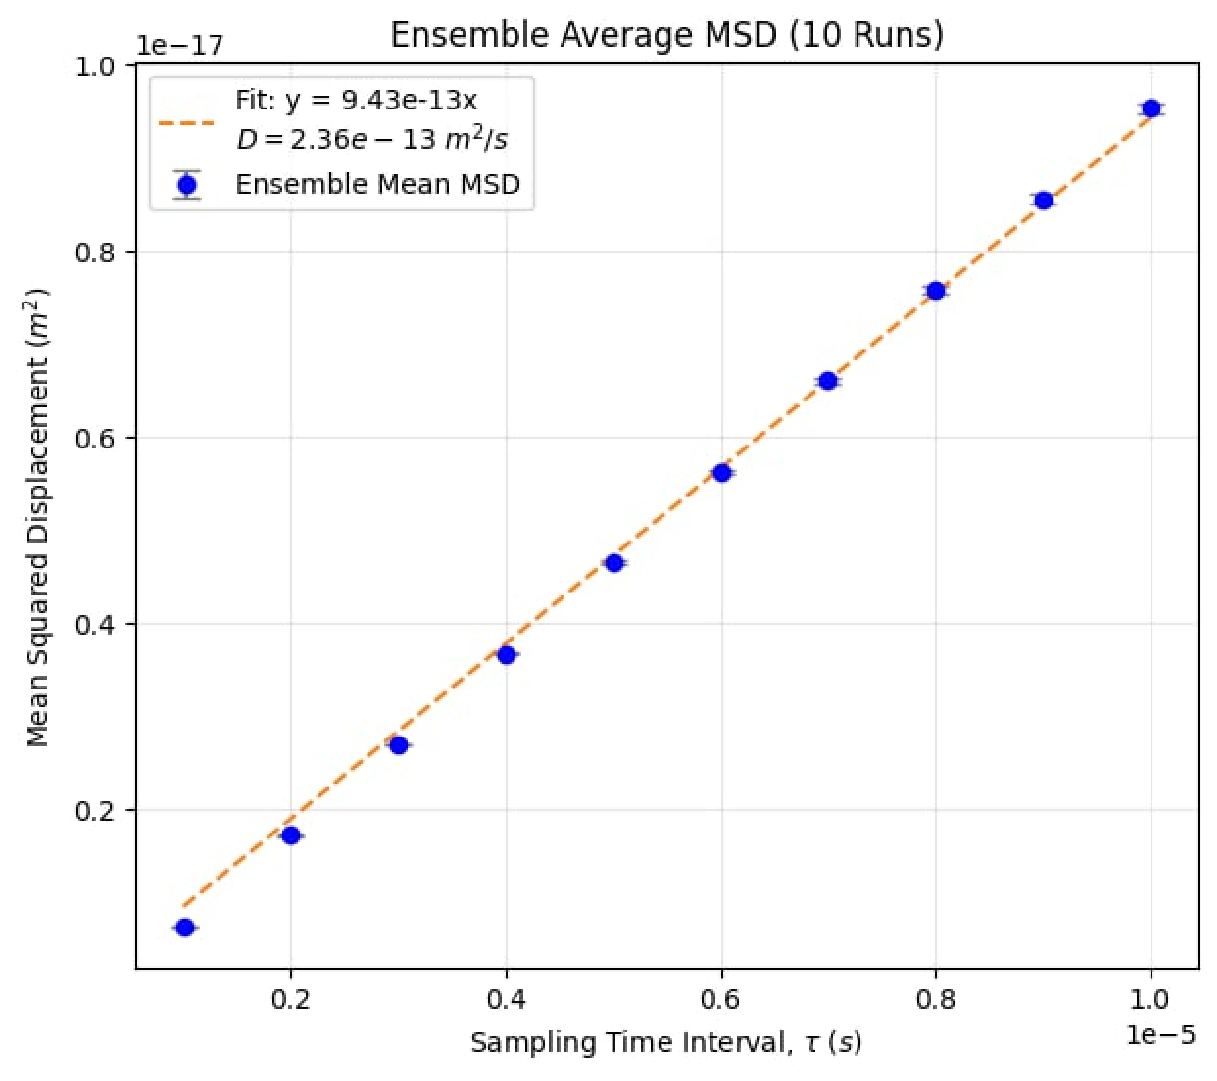
\includegraphics[width=0.48\textwidth]{figures/Probe_MSD.pdf}
    \hfill 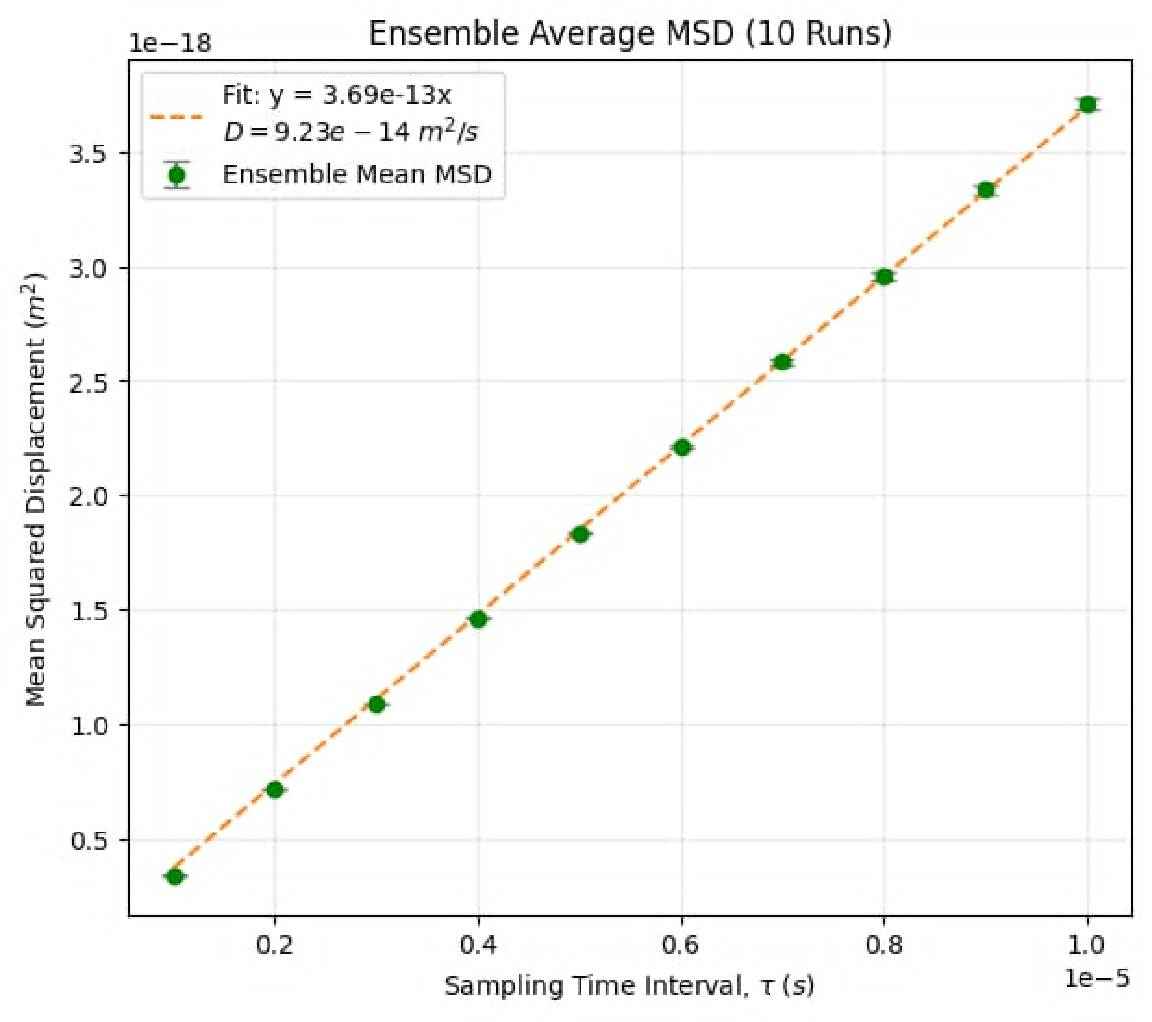
\includegraphics[width=0.48\textwidth]{figures/Foreign_MSD.pdf}
    
    \caption{Ensemble-average mean squared displacement versus sampling interval $\tau$ for the (a) probe and (b) foreign particle species, with linear fits used to extract $D_\text{MSD}$.}
    \label{fig:side_by_side_plots}
\end{figure}

\begin{equation}
    D_{var} = \frac{\sigma_x^2+ \sigma_y^2}{2d\tau} = \frac{\sigma_x^2+ \sigma_y^2}{4\tau}
\label{eqn:1.6}
\end{equation}

% To fix, I will make the plots 2x2 so it will be bigger
% \begin{figure}[b]
%     \centering
%     \subfigure{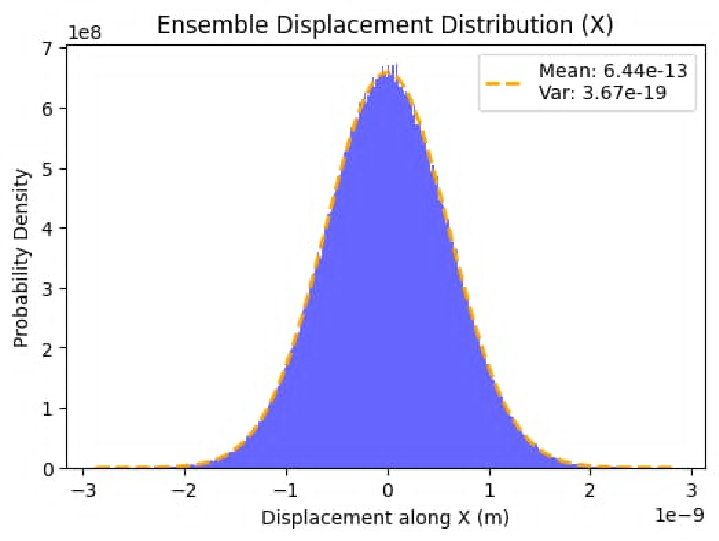
\includegraphics[width=0.25\textwidth]{figures/Probe_Disp_X.pdf}%
%     }%
%     \hfill
%     \subfigure{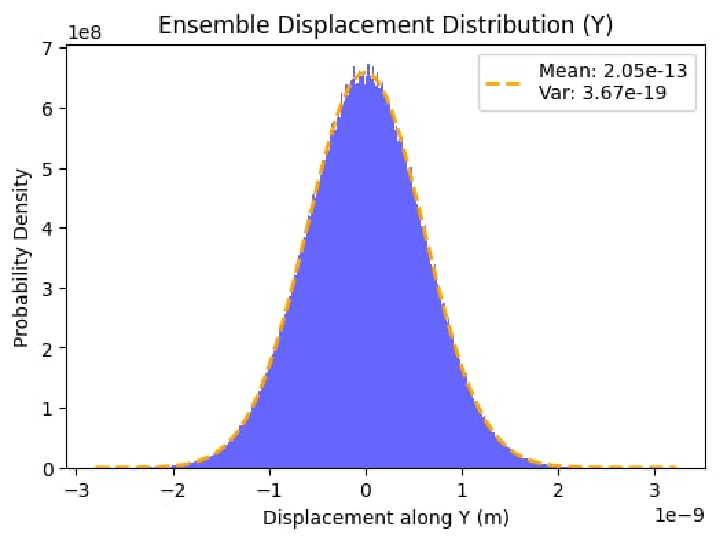
\includegraphics[width=0.25\textwidth]{figures/Probe_Disp_Y.pdf}%
%     }%
%     \hfill
%     \subfigure{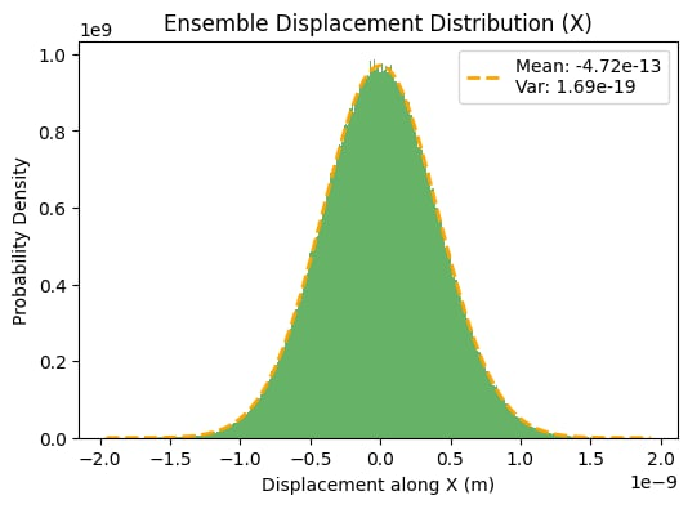
\includegraphics[width=0.25\textwidth]{figures/Foreign_Disp_X.pdf}%
%     }%
%     \hfill
%     \subfigure{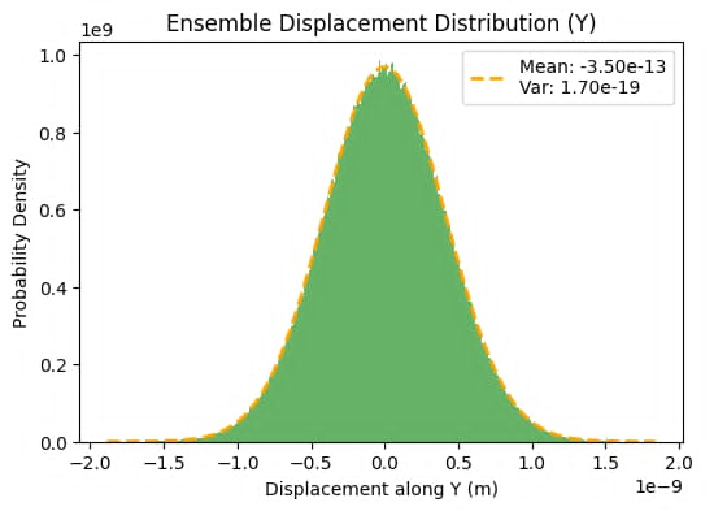
\includegraphics[width=0.25\textwidth]{figures/Foreign_Disp_Y.pdf}%
%     }%
    
%     \caption{Ensemble displacement distribution along x for the (a) probe and (b) foreign particle species, with Gaussian fits confirming the CLT-predicted profile used to extract $D_\text{var}$}
%     \label{fig:four_plots}
% \end{figure}
\begin{figure}[h]
    \centering
    % Top Row
    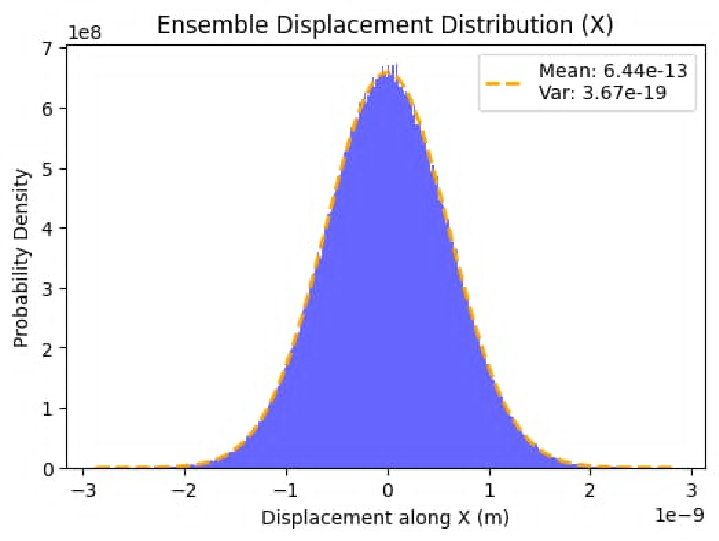
\includegraphics[width=0.48\textwidth]{figures/Probe_Disp_X.pdf}%
    \hfill
    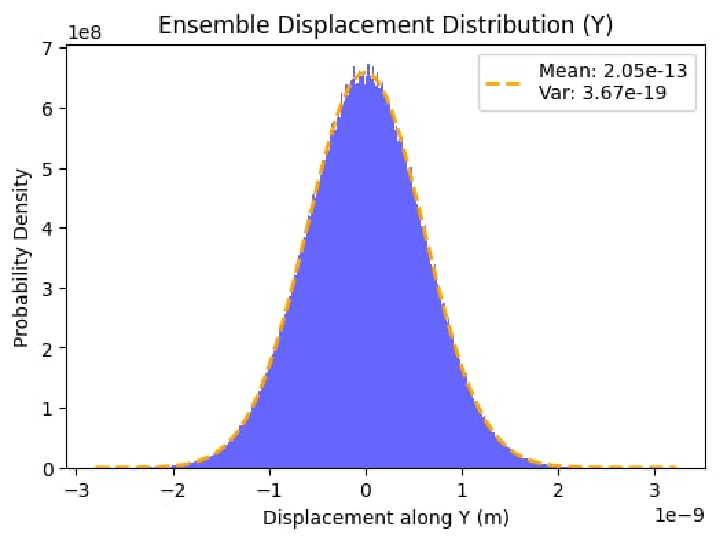
\includegraphics[width=0.48\textwidth]{figures/Probe_Disp_Y.pdf}%
    \\[0.5em] % Vertical space between top and bottom rows
    % Bottom Row
    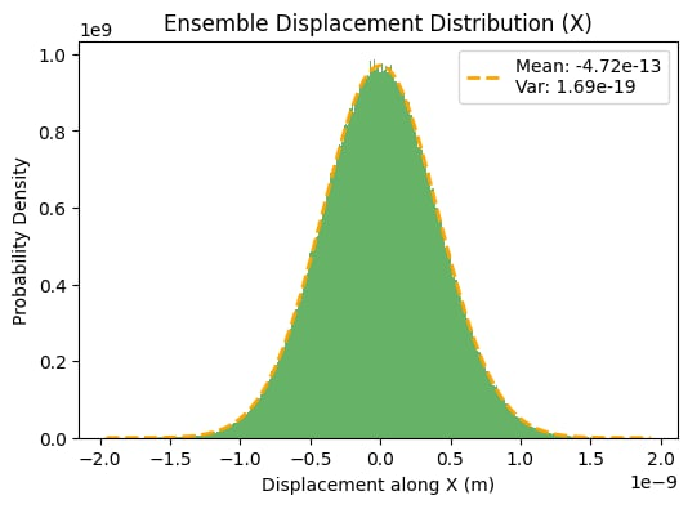
\includegraphics[width=0.48\textwidth]{figures/Foreign_Disp_X.pdf}%
    \hfill
    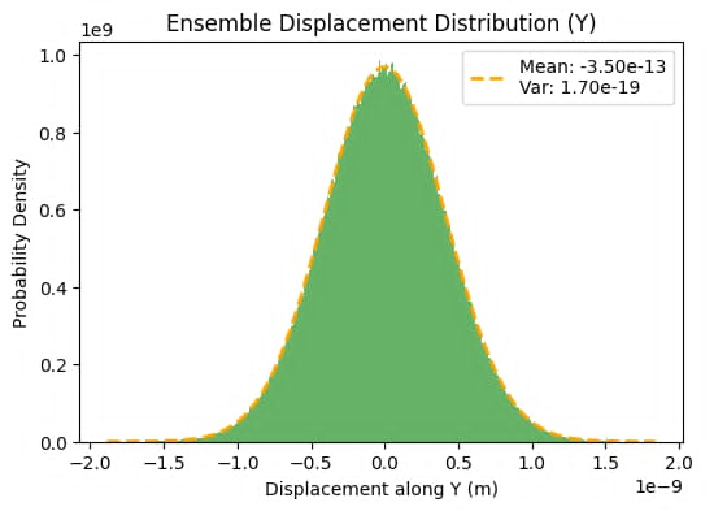
\includegraphics[width=0.48\textwidth]{figures/Foreign_Disp_Y.pdf}%
    
    \caption{Ensemble displacement distributions along $x$ and $y$ for the probe and foreign particle species, with Gaussian fits confirming the CLT-predicted profile used to extract $D_\text{var}$.}
    \label{fig:four_plots}
\end{figure}

\noindent ensuring that the sampling time $\tau$ is significantly longer than the Langevin damping parameter ($\tau >> \tau_{damp}$) is essential to avoid the deterministic ballistic motion regime ($\tau \leq \tau_{damp}$) and achieve precise agreement with the theoretical Stoke-Einstein diffusion coefficient \cite{Einstein1956, balejado2025}:

\begin{equation}
    D_T = \frac{k_BT}{6\pi\eta r},
\label{eqn:1.7}
\end{equation}

\noindent where $k_B$ is the Boltzmann constant and $T$ is absolute temperature.

\hspace{\parindent} When $N_p$ Brownian polystyrene probe particles wander inside a domain containing target foreign particles, the primary physical quantity of interest is the first-passage detection time $T$. This is defined as the time step at which any probe particle first comes within a specified interaction distance $R_{int}$ of a foreign target particle, accounting for the collision cross section $\sigma_{\alpha \beta}$ \cite{Redner2001}. When probe density is low, probes do not interfere with each other. Under the Ergodic Theorem \cite{Zwanzig2001}, the ensemble average across searchers is equivalent to the time average of a single searcher exploring space over an extended duration. Consequently, $\langle T\rangle \propto \frac{1}{N_p}$, meaning the Ergodic Product $E = N_p \times \langle T \rangle$ remains constant \cite{Loverdo2008}. When the Ergodic Product $E$ remains flat across varying probe counts, the system operates within the ergodic, diffusion-limited search regime.

\hspace{\parindent} As $N_p$ grows, the total occupied surface area increases. The system density is measured by its Area Fraction ($\phi$) \cite{Balejado2026}:

\begin{equation}
    \phi = \frac{N_p \pi r_p^2 + N_f \pi r_f^2}{A_{box}},
\label{eqn:1.8}
\end{equation}

\noindent where $N_p$ and $r_p$ are the number and radius of probe particles, $N_f$ and $r_f$ are the number and radius of foreign target particles, and $A_{box} = L \times L$ is the area of the square box subject to periodic boundary conditions. To prevent physical overlap between finite-sized particles, short-range repulsive interactions are modeled using the Weeks-Chandler-Andersen (WCA) soft repulsion potential \cite{Weeks1971}:

\begin{equation}
    U_{WCA}(r) = \begin{cases}
        4\mathcal{E}\left[\left(\frac{\sigma}{r}\right)^12-\left(\frac{\sigma}{r}\right)^6\right] + \mathcal{E}, &r\leq2^{1/6}\sigma \\
        0, & r\geq 2^{1/6}\sigma
    \end{cases},
\label{eqn:1.9}
\end{equation}

\noindent where $\varepsilon$ sets the interaction energy scale and $\sigma$ represents the effective hard-core collision diameter. As $\phi$ increases toward dense packing regimes, probes frequently collide with neighbors, causing available free space to contract and trapping particles inside temporary cages \cite{Weeks2000}. This transition marks the boundary of the crowding-limited search regime, where adding more probes increases $\langle T\rangle$ and causes $E$ to deviate upward from linearity.

\section{Statement of the Problem}
\label{sec:1.3}
\hspace{\parindent} In microscopic search and capture systems, maximizing detection speed while managing the concentration of probes is a primary practical challenge. While adding searchers accelerates detection times in open fluids, deploying excess probe particles in confined or dense environments triggers steric hindrance, reduces diffusive mobility, and increases detection times \cite{Torquato2002, Weeks2000}. Although first-passage dynamics in dilute media are well established theoretically \cite{Redner2001}, a number of key questions remain open regarding crowded, multi-sized non-equilibrium mixtures.

\hspace{\parindent} Specifically, this study addresses how varying probe density directly impacts mean first-passage detection times ($\langle T\rangle$) across different system scales ($N_{total}$). It determines the exact area fraction ($\phi$) threshold where a two-dimensional Brownian system transitions from a diffusion-limited search to a crowding-limited search. Furthermore, it investigates whether the Ergodic Product ($E = N_p \times \langle T\rangle$) can serve as an earlier, more sensitive order parameter for detecting the onset of spatial crowding compared to monitoring $\langle T \rangle$ alone, while evaluating how overall system scale modifies the physical detection limit in crowded colloidal environments \cite{Balejado2026}. As part of characterizing this transition, this thesis also proposes a fourfold qualitative typology for classifying how sharply the crowding-limited response manifests as a function of system scale with the typology consisting of Incipient, Shield, and Steep-Walled, and the Bifurcated caldera profiles.


\section{Objectives of the Study}
\label{sec:1.4}
\hspace{\parindent} The study uses two-dimensional Brownian dynamics simulations to analyze how probe density and excluded-volume crowding affect first-passage target detection efficiency. The primary objective is to construct particle-based Brownian dynamics simulations in \texttt{LAMMPS} modeling non-equilibrium mixtures of polystyrene probe particles ($d_p = 2.0\, \mu$m) and foreign target particles ($d_f = 1.0 \,\mu$m) under periodic boundary conditions \cite{Thompson2022}. Pure Brownian dynamics are verified by calculating diffusion coefficients via both Mean Squared Displacement ($D_{MSD}$) and Displacement-Variance ($D_{var}$) techniques, validating them against theoretical Stokes-Einstein predictions ($D_{th}$) \cite{Einstein1956, Cusi2020, balejado2025}.

\hspace{\parindent} Furthermore, this work quantifies the Mean First-Passage Detection Time ($\langle T \rangle$) across a wide range of probe numbers ($N_p$) and system ensemble sizes ($N_{total} = 10, 30, 50, 70, 100, 200$) across multiple independent simulation seeds. The ergodic product ($E = N_p \times \langle T \rangle$) is evaluated as a diagnostic parameter to pinpoint the exact transition from ergodic diffusion-limited dynamics to non-ergodic crowding-limited dynamics \cite{Loverdo2008}. Finally, this study identifies the optimal probe density window that maximizes foreign target detection efficiency before caging effects impair probe mobility. 

\section{Significance of the Study}
\label{sec:1.5}
\hspace{\parindent} This work provides insights across physics, biophysics, soft condensed matter, and bio-nanotechnology. Biological cells are packed with macromolecules occupying $20\,\%$ to $40\,\%$ of cellular volume \cite{Loverdo2008, Benichou2011}. This study provides a framework for understanding how crowding alters reaction rates, search strategies, and transport efficiency inside living cytoplasm \cite{Loverdo2008, Redner2001}.

\hspace{\parindent} In automated point-of-care microfluidic diagnostic devices, functionalized magnetic or polystyrene beads are introduced to detect rare pathogens or trace analytes. Determining the optimal probe density prevents fluid clogging and minimizes diagnostic detection times while reducing reagent costs. From a theoretical perspective, by testing the breakdown of the Ergodic Theorem in soft-core particle suspensions, this research contributes to the fundamental understanding of non-equilibrium statistical mechanics, glassy caging dynamics, and multi-agent stochastic search optimization \cite{Redner2001, Zwanzig2001, Weeks2000}.

\section{Scope and Limitation of the Study}
\label{sec:1.6}
\hspace{\parindent} To ensure a focused physical investigation, the parameters and computational boundaries of this study are defined carefully. Simulations are restricted to two-dimensional (2D) square spatial domains with periodic boundary conditions, mimicking thin fluid films, microfluidic chips, or biological membrane surfaces. Probes are modeled as polystyrene spheres with diameter $d_p = 2.0 \,\mu$m, while foreign target particles have diameter $d_f = 1.0\,\mu$m, maintaining a $2:1$ diameter ratio. Particle mass density is set to $\rho = 1050$ \,kg/m$^3$ in water at $T = 298\,$K ($\eta = 0.89\,$mPa$\cdot$s).

\hspace{\parindent} interparticle collisions are modeled strictly via short-range repulsive Weeks-Chandler-Andersen (WCA) potentials \cite{Weeks1971}. Long-range electrostatic charges, hydrodynamic interactions between moving spheres, and particle gravity or buoyancy effects are excluded. Computational trajectories are generated using \texttt{LAMMPS} \cite{Thompson2022}, visualized using \texttt{OVITO} (Open Visualization Tool) \cite{Stukowski2010}, and post-processed using custom \texttt{Python} analysis workflows using \texttt{NumPy}, \texttt{SciPy}, and \texttt{Matplotlib}.
% !TEX root =  main.tex
\chapter{The Detection Challenge}
\label{chap:2}

\section{From Pollen Grains}
\label{sec:2.1}
\hspace{\parindent} The Brownian Motion story begins with a mystery no one could explain. In 1827, the botanist Robert Brown watched pollen grains suspended in water twitch under his microscope with no apparent cause, and reported the observation without being able to account for it \cite{Brown1828}. For nearly seventy-eight years the jiggling carried his name but no accepted mechanism. Albert Einstein supplied one explanation in 1905, arguing ceaselessly battering the suspended grain from random directions \cite{Einstein1905, Einstein1956}. Marian Smoluchowski arrived at an equivalent picture independently around the same time \cite{Smoluchowski1906}. What made Einstein's account more than a plausible story was that it made a number falsifiable: it predicted how far, on average, a particle of known size should wander in a fluid of known viscosity and temperature. Jean Perrin tested that prediction directly under the microscope a few years later, and the resulting agreement was treated as some of the strongest available evidence that atoms and molecules were physically real rather than a convenient bookkeeping device \cite{Perrin1916}.

\hspace{\parindent} Paul Langevin gave the same physics a different, and for simulation purposes more usable form. Rather than track a probability distribution, he wrote down a force equation for a single particle: a drag term that always opposes motion, plus a rapidly fluctuating random force representing the unresolved molecular collisions \cite{Coffey2004}. This is the Langevin equation already introduced in Section~\ref{sec:1.2}, and it is the equation LAMMPS integrates, through its \texttt{fix langevin} command, for every probe and foreign particle in this thesis' simulations. Ornstein and Uhlenbeck later worked out the statistical consequences of that equation in full: over sampling intervals much longer than the particle's momentum relaxation time, displacements settle into a zero-mean Gaussian distribution \cite{Uhlenbeck1930}. That single result is what makes two independent measurement strategies possible later in this thesis where one can either measure how far particles spread out on average through the mean squared displacement route or measure the shape of the displacement distribution itself through the use of the variance route, and both should recover the same diffusion coefficient if the motion is truly Brownian.

\section{Two ways to Measure the Same Number}
\label{sec:2.2}
\hspace{\parindent} Knowing that Brownian motion should be Gaussian and diffusive is not the same as being able to extract a clean diffusion coefficient from a finite, noisy simulated or experimental trajectory. This is where the Brownian group's own prior work becomes directly irrelevant. Cusi, Tapang, and Saloma first examined how probe-probe collisions corrupt diffusion coefficient measurements in dilute suspensions \cite{Cusi2018}, then followed up with a systematic comparison of the two extraction methods: reading the diffusion coefficient off the slope of the mean squared displacement (MSD) curve, $D_\text{MSD}$, versus reading it off the variance of the displacement distribution, $D_\text{var}$ \cite{Cusi2020}. Cusi's undergraduate thesis extended this further into an experimental single-particle tracking study, and identified spatial resolution, which is how finely a camera can resolve a particle's position, as the single most influential factor governing whether a measured diffusion coefficient can be trusted \cite{Cusi2020Thesis}. Around the same period, Michalet and Berglund arrived at a related conclusion from a more theoretical direction, showing that the accuracy of diffusion coefficient estimates from tracked trajectories depends sensitively on how the fit is constructed, not just on how good the raw data are \cite{Michalet2012}.

\hspace{\parindent} The immediate predecessor to this thesis, Balejado, Escaran, Cusi, and Saloma's 2025 conference paper, asked a narrower and more pointed questions: given that $D_\text{MSD}$ and $D_\text{var}$ should agree in principle, at what sampling time interval $\tau$ do they actually agree in LAMMPS simulation \cite{balejado2025} The answer hinges on the Langevin damping parameter $\tau_\text{damp}$, the characteristic time over which a particle forgets its own momentum through viscous drag. Sampling faster than $\tau_\text{damp}$ catches the particle still moving ballistically along its last random kick, which biases both methods low; sampling much slower than $\tau_\text{damp}$ recovers the correct diffusive value but shortens the usable trajectory and inflates statistical noise. Related diagnostic work along the same lines, focused specifically on the reliability of computed diffusion coefficients and their uncertainties, was carried out by McCluskey, Coles, and Morgan \cite{McCluskey2023}. The practical result for this thesis is a design rule rather than a debate: choose $\tau \gg \tau_\text{damp}$ before trusting a single measurement, and confirm the simulation is behaving as pure Brownian motion before asking any question about detection. Chapter~\ref{chap:3} follows exactly that rule.


\section{The Detection Problem: How Long Until Something is Found?}
\label{sec:2.3}
Diffusion theory describes how a particle spreads out; it does not, by itself, say when that particle will first reach a specific target. That question belongs to a distinct body of work known as first-passage or search theory, laid out comprehensively by Redner \cite{Redner2001} and extended to biological chemical search problems by B\'enichou, Loverdo, Moreau, and Voituriez \cite{Loverdo2008, Benichou2011}. Their central result, already stated as Equation~\ref{eqn:1.1}, is deceptively simple where if a lone searcher takes an average time $\langle T \rangle$ to find a target, then $N_p$ independent, non-interacting searchers should find it in $\langle T \rangle / N_p$ on average. Condamin and colleagues showed that this scaling holds even in geometrically complicated, scale-invariant search spaces \cite{Condamin2007}, while B\'enichou and their collaborators demonstrated that the geometry of the search domain itself can be tuned to control how quickly a target is found \cite{Benichou2010}. Two features of this literature matter directly for this thesis. First, the $1/N_p$ law is explicitly an \emph{ideal-limit} statement, valid only while searchers genuinely do not interfere with one another; nothing in the theory says what happens once they do. Second, the law rests on ergodicity, the idea that averaging over many independent searchers observed briefly gives the same answer as averaging over one searcher observed for a proportionally longer time. The ergodic product, $E = N_p \times \langle T \rangle$, used throughout this thesis, is simply a way of putting that assumption to a direct test and if it holds, $E$ should sit flat against $N_p$, and any systematic drift is evidence that the searchers have stopped behaving independently.

\section{Crowding and Caging}
\label{sec:2.4}
\hspace{\parindent} The search theory literature is largely built for dilute systems, where adding a searcher costs nothing but its own trajectory. Real search environments rarely stay dilute once enough searchers are added, and a separate body of work in soft condensed matter physics describes what happens when they do not. Weeks, Crocker, Levitt, Schofield, and Weitz used three-dimensional microscopy of colloidal suspensions to directly visualize the onset of caging where as particle packing increases toward the colloidal glass transition, each particle becomes increasingly hemmed in by its neighbors, and its mobility drops sharply even though nothing has frozen in the conventional sense \cite{Weeks2000}. Torquato's treatment of random heterogeneous materials provides the geometric backbone for quantifying how densely particles can be packed before free space effectively disappears, including the hexagonal close packing bound $\phi_\text{HCP} = \pi/(2\sqrt{3}) \approx 0.9069$ used as a reference ceiling in Section~\ref{sec:1.2} \cite{Torquato2002}. The physical intuition these two works supply is what motivates the crowding-limited regime described in this thesis where past some area fraction $\phi$, newly added probes do not meaningfully explore new space, they mostly collide with, and get boxed in by, the probes and foreign particles that are already there. This is the same physical mechanism, expressed through the excluded-volume repulsion of the Weeks-Chandler-Andersen (WCA potential \cite{Weeks1971}, that ultimately produces the upturn in $\langle T \rangle$ at high $N_p$ documented in Balejado, Tapang, and Saloma's 2026 conference paper \cite{Balejado2026} and revisited at greater depth in this thesis. 

\section{LAMMPS}
\label{sec:2.5}
\hspace{\parindent} None of the above would be testable at scale without the reliable simulation engine. This thesis uses the Large-scale Atomic/Molecular Massively Parallel Simulator (LAMMPS), a particle-based molecular dynamics code originally developed for materials science but widely repurposed for soft-matter and colloidal simulation because of its flexible pairwise potentials and built-in Langevin thermostat features \cite{Thompson2022}. Visual inspection and rendering of the resulting particle trajectories, which is useful during the development and debugging phase, relied on OVITO, the Open Visualization Tool \cite{Stukowski2010}.

\hspace{\parindent} One further statistical tool deserved mention because it plays a direct role in Chapter~\ref{chap:4}'s presentation of results which is the violin plot. A conventional error bar communicates only a mean and a spread, and can look identical whether the underlying detection times are tightly clustered, evenly spread, or badly skewed with a long tail of rare, very slow detections. Hintze and Nelson introduced the violin plot precisely to solve this problem, combining a traditional box-plot summary with a mirrored kernel density trace so that the full shape of a distribution, not just its first two moments, is visible at a glance \cite{Hintze1998}. Given that this thesis specifically expects detection time distributions to change shape, from tight and symmetric in the diffusion-limited regime to broad and right-skewed once caging sets in, the violin plot is not a cosmetic choice but a diagnostic one, and it is treated as such in the results and discussion chapter.

\section{The Study Gap this Thesis Addresses}
\label{sec:2.6}
\hspace{\parindent} Taken together, the literature above supplied every ingredient except the one this thesis contributes. Search theory gives the ideal $1/N_p$ scaling law and the ergodic product as its diagnostic. Colloidal physics gives the caging mechanism that should eventually break that law. Our group's own prior work gives a validated LAMMPS pipeline and a settled, damping-parameter-aware protocol for extracting trustworthy diffusion coefficients. What had not yet been done, at the start of this project, was to put a size-varying, two-species, WCA-repulsive Brownian mixture through the full range of probe densities, from a single lonely searcher up to a near-close-packed swarm, and ask exactly where along that range the diffusion-limited and crowding-limited regimes meet, and whether the ergodic product can flag that transition earlier than tthe raw detection time can. That question, first posed in preliminary form in \cite{Balejado2026}, is the one that this thesis answers in full, across multiple systet sizes $N_\text{total}$, in Chapters~\ref{chap:3} and~\ref{chap:4}.
% !TEX root =  main.tex
\chapter{The Detection Methodology}
\label{chap:3}
Chapter~\ref{chap:2} closed on a specific, and still-open question: across a wide sweep of probe number $N_p$, where exactly does a two-dimensional Brownian search system stop behaving like a collection of independent searchers, and can the ergodic product $E = N_p \times \langle T \rangle$ catch that moment earlier than the raw mean detection time $\langle T \rangle$ can? This chapter lays out, step by step, how that question was turned into a concrete, repeatable simulation and analysis pipeline: how the simulated system was built, how its particles were made to move like real Brownian probes, how a ``detection" was defined and times, and how the resulting numbers were turned into the statistics reported in the results and discussion chapter.

\section{Non-Equilibrium Mixtures}
\label{sec:3.1}
Every simulation in this study models the same basic scene: a flat, square, two-dimensional box populated by two kinds of particles that never chemically react or convert into one another, but that constantly push each other around through short-range collisions. This qualifies as a \textbf{non-equilibrium mixture}: unlike a gas of identical molecules at thermal equilibrium, the two species here differ in size and in how strongly they are damped by the fluid, so the system has no single, symmetric equilibrium state to relax into so it is simply driven, indefinitely, by thermal noise. The two species are:

\begin{itemize}
  \item \textbf{Polystyrene probe particles} ($N_p$), diameter $d_p = 2.0~\mu\text{m}$, playing the role of the searchers; and
  \item \textbf{Foreign particles} ($N_f = N_\text{total} - N_p$), diameter $d_f = 1.0~\mu\text{m}$, representing the impurity being searched for.
\end{itemize}

Rather than fixing the total particle count and varying only $N_p$, this thesis repeats the entire sweep at six different values of total number of particle in the system $N_\text{total}$ (10, 30, 50, 70, 100, and 200), so that any trend identified is checked for consistency across system size rather than being an artifact of one particular box. For each $N_\text{total}$, $N_p$ is swept from a single lone probe up to nearly the full population, using the same fractional schedule in every case: $N_p$ is set to 1, 2, 3, \ldots, 9, then 10\%, 20\%, \ldots, 90\%, 95\%, and 99\% of $N_\text{total}$, rounding to the nearest whole particle and never letting $N_p$ fall below 1. This is the same probe-density sweep implemented directly in the LAMMPS input script through the nested \texttt{loop\_percent} and \texttt{loop\_seed} loops, and it is what allows the same set of area fractions to be revisited, system after system, in Chapter~\ref{chap:4}.

\section{Area Fraction and the Packing Ceiling}
\label{sec:3.2}
The single number used throughout this thesis to describe how ``full'' the box is, at any given $N_p$, is the \textbf{area fraction} $\phi$, already defined in Equation~\ref{eqn:1.8} as the fraction of the box's total area physically occupied by particles:

\begin{equation}
    \phi = \frac{N_p \pi r_p^2 + N_f \pi r_f^2 }{A_\text{box}}, \qquad A_\text{box} = L \times L
    \label{eq:3.1}
\end{equation}

Because $r_p \neq r_f$, $\phi$ changes with $N_p$ even at fixed $N_\text{total}$, which is why every figure in Chapter~\ref{chap:4} carries a second horizontal axis converting $N_p$ into $\phi$. As a sanity ceiling, no simulated system in this thesis is ever allowed to approach the theoretical two-dimensional hexagonal
close packing (HCP) fraction, $\phi_\text{HCP} = \pi/(2\sqrt{3}) \approx 90.7\%$ (Section~\ref{sec:1.2}); the highest area fractions actually reached, near $\phi \approx 48\%$, sit well below that geometric limit, meaning the crowding effects reported in Chapter~\ref{chap:4} are a dynamical, caging-driven phenomenon and not simply a consequence of running out of physical space.

\section{Box Size and Periodic Boundary Conditions}
\label{sec:3.3}
For each $N_\text{total}$, the box side length $L$ was fixed in advance so that sweeping $N_p$ from 1 to $N_\text{total}-1$ traces out the same, comparable range of area fractions (roughly 12\% to 48\%) regardless of system size. The six box sizes used were $L = 8.03$, $13.9$, $17.96$, $21.26$, $25.4$, and $35.92~\mu\text{m}$ for $N_\text{total} = 10, 30, 50, 70, 100$, and $200$ respectively. Every box uses \textbf{periodic boundary conditions} (PBC) where a particle that exits through the right edge of the box re-enters through the left edge, and likewise for the top and bottom, so that the simulated patch of fluid behaves as if it were one tile in an infinitely repeating grid rather than a container with hard, particle-repelling walls (which often results in the simulation blowing up). This choice removes wall effects from the physics being studied and is what makes the \textbf{minimum image convention}, described in Section~\ref{section:3.4}, necessary when measuring distances between particles.

\section{Simulation Settings and Particle Parameters}
\label{section:3.4}
All simulations were run in LAMMPS \cite{Thompson2022}, using two-dimensional spherical particles (\texttt{atom\_style sphere}, \texttt{dimension 2}) at a fixed \textbf{mass density} of $\rho = 1050~\text{kg/m}^3$, matching real polystyrene microspheres in water and consistent with the group's earlier
diffusion-coefficient work \cite{Cusi2018, balejado2025}. The surrounding fluid is water at $T = 298~\text{K}$, with a \textbf{viscosity} of $\eta = 0.89~\text{mPa·s}$; viscosity enters the simulation not as an explicit force field but implicitly, through the Langevin damping parameter described next.

\section{The Langevin Damping Parameter}
\label{sec:3.5}
Every probe and foreign particle is driven by a Langevin thermostat (\texttt{fix langevin}), which realizes the stochastic equation of motion introduced in Section~\ref{sec:1.2}: a viscous drag term plus a random thermal kick. The strength of the drag is set by the \textbf{Langevin damping parameter} given by,

\begin{equation}
  \tau_\text{damp} = \frac{m}{6 \pi \eta r},
  \label{eq:3.2}
\end{equation}

the characteristic time over which a particle's own momentum is erased by collisions with the fluid. For the $2.0~\mu\text{m}$ probe, this works out to $\tau_\text{damp} \approx 0.262~\mu\text{s}$, and the LAMMPS input script sets this value directly as the \texttt{damp} argument of \texttt{fix langevin} for the probe group. The foreign particles, being smaller, are assigned a shorter damping time of $0.1~\mu\text{s}$. Unlike the probe's $\tau_\text{damp}$, which is computed directly from Equation~\ref{eq:3.2}, the foreign particle's damping time was set deliberately rather than calculated from its Stokes radius: a round value of $0.1\,\mu$s, ensuring the smaller species equilibrates into the diffusive regime at least as quickly as the probe and does not become the limiting timescale for the $\tau \gg \tau_\text{damp}$ criterion applied uniformly in Section~\ref{sec:3.7}. This parameter is not a free dial; it is the same quantity whose mishandling was shown, in the group's prior sampling-interval study \cite{balejado2025}, to silently bias diffusion coefficient measurements low when the simulation is sampled too quickly. Its role is revisited directly in Section~\ref{section:3.4}.

\section{The Three-Stage LAMMPS Protocol}
\label{sec:3.6}
Simply dropping $N_\text{total}$ particles into the box at random, at the target density, would leave many of them overlapping, which is physically meaningless and numerically unstable. Instead, each run proceeds through three distinct stages.

\subsection{Stage 1: Overlap Removal}
\label{sec:3.6.1}
Particles are first placed at random positions inside an oversized box, four times the linear dimension of the final target box ($4L \times 4L$, via the \texttt{expand} variable). A soft, purely repulsive potential (\texttt{pair\_style soft}) gently pushes overlapping particles apart over 50,000 timesteps, with particle velocities capped (\texttt{fix nve/limit}) to prevent the sudden, unphysical accelerations that would otherwise occur if two particles happened to start on top of one another.

\subsection{Stage 2: Compression} 
\label{sec:3.6.2}
With no more overlaps, the box is compressed from $4L \times 4L$ down to the final $L \times L$ target size over a further 100{,}000 steps (\texttt{fix deform}), again under the soft potential and velocity limiting, so that particles are squeezed toward their intended packing density gradually rather than being teleported into a suddenly crowded box.


\subsection{Stage 3: Production - Weeks-Chandler-Andersen Repulsion and Brownian Dynamics}
\label{sec:3.6.3}
Only in the final, production stage are the particles switched onto the physics this thesis actually studies. The soft potential is replaced by the \textbf{Weeks-Chandler-Andersen (WCA) potential} (Equation~\ref{eqn:1.9}), implemented in LAMMPS as a Lennard-Jones potential (\texttt{pair\_style lj/cut}) truncated at its energy minimum and shifted to zero at the cutoff (\texttt{pair\_modify shift yes}), so that particles feel a purely repulsive excluded-volume force and nothing attractive. Each Langevin fix is left active, now driving genuine Brownian motion rather than merely relaxing overlaps. The production run integrates $2.0 \times 10^{8}$ steps at $\Delta t = 0.01~\mu\text{s}$, giving a total simulated time of $2.0~\text{s}$ per run, with particle positions written to disk (\texttt{dump}) every 100 steps, i.e. every $\tau = 1.0~\mu\text{s}$ of simulated time. Every ($N_\text{total}$, $N_p$) combination described in Section~\ref{sec:3.1} is repeated across 10 independent random seeds, so that the mean detection time reported for each condition in Chapter~\ref{chap:4} is itself an average over 10 statistically independent realizations of the same physical setup, not a single run.

\section{Verifying Pure Brownian Dynamics}
\label{sec:3.7}
\begin{figure}[h]
    \centering
    \includegraphics[width = 0.95\linewidth]{figures/2Dtrajectory.pdf}
    \caption{Representative unwrapped 2D trajectory of a probe particle (type 1) and a foreign particle (type 2) during the production stage, illustrating undirected Brownian motion with no systematic drift.}
    \label{fig:2Dtrajectory}
\end{figure}

\noindent Before any detection-time measurement can be trusted, the simulation itself has to be shown to be doing what it claims: moving each particle species by pure, undirected Brownian motion, not some artifact of an ill-chosen timestep. This verification step, standard practice established in the group's prior work \cite{Cusi2020, balejado2025}, uses two independent estimators of the \textbf{diffusion coefficient} $D$ (Section~\ref{sec:1.2}), computed from particle trajectories collected during production (Figure \ref{fig:2Dtrajectory}):

\begin{align}
  \text{MSD}(\tau) &= \left\langle \left[\mathbf{r}(t+\tau) - \mathbf{r}(t)\right]^2 \right\rangle = 2dD_\text{MSD}\,\tau,
  \label{eq:3.3} \\
  D_\text{var} &= \frac{\sigma_x^2 + \sigma_y^2}{2d\tau},
  \label{eq:3.4}
\end{align}

where $d = 2$ for the two-dimensional systems used here. Both are checked against the theoretical Stokes-Einstein value, $D_\text{th} = k_B T / (6\pi\eta r_p) \approx 0.245~\mu\text{m}^2/\text{s}$ for the probe. Critically, this comparison is only meaningful at a \textbf{sampling time interval} $\tau$ chosen to satisfy $\tau \gg \tau_\text{damp}$: the group's earlier work showed that sampling at or below $\tau_\text{damp}$ catches particles still in their ballistic, momentum-dominated regime, which biases both $D_\text{MSD}$ and $D_\text{var}$ low regardless of how long the trajectory is \cite{balejado2025}. With $\tau_\text{damp} \approx 0.262~\mu\text{s}$ for the probe and a chosen dump interval of $\tau = 1.0~\mu\text{s}$, this thesis operates safely inside the diffusive regime, and both diffusion estimators are confirmed to agree with $D_\text{th}$ before any detection statistics are computed.

For the foreign particle, the theoretical Stokes-Einstein prediction is $D_\text{th} \approx 9.3\times 10^{-14} \,m^2$/s, compared with $D_\text{MSD} \approx 9.23\times10^{-14}\, m^2$/s and $D_\text{var} = 8.46\times10^{-14}\,m^2$/s extracted from the trajectories (Figure~1.2), showing agreement to within a few percent for $D_\text{MSD}$ and somewhat looser agreement for $D_\text{var}$. Take note as well that because $\tau_{damp}$ for the foreign species was fixed at $0.1\,\mu$s for computational efficiency, its $D_{th}$ is $0.091\,\mu\text{m}^2/s$ rather than $0.490\,\mu\textbf{m}^2/s$ (which pure Stokes-Einstein scaling would predict for $r=0.5\,\mu$m). Together with the probe's own agreement, both species are confirmed to be undergoing pure diffusive Brownian motion at the chosen sampling interval before any detection statistics are computed.

\section{Defining and Extracting the First-Passage Detection Time}
\label{sec:3.8}
With Brownian motion confirmed, the next task is to decide, precisely, what counts as a ``detection.'' A probe is considered to have detected a target the first instant it comes within a fixed \textbf{interaction radius}, $R_\text{int} = 1.5~\mu\text{m}$, of any foreign particle. This radius stands in for the physical \textbf{collision cross section} $\sigma_{\alpha\beta}$ introduced in Section~\ref{sec:1.2}: rather than requiring the two particles' surfaces to touch exactly, $R_\text{int}$ defines a slightly generous capture zone around each foreign particle, representing the effective range over which a real sensor or reactive site would register contact. Because the simulation box is periodic,
computing the distance between a probe and a foreign particle na\"ively (by simple coordinate subtraction) would be wrong whenever the two happen to sit on opposite sides of the box, since periodic images can be much closer than the raw coordinates suggest. Every distance calculation therefore applies the \textbf{minimum image convention}, wrapping each coordinate difference into the range $[-L/2, L/2]$ before computing distance, so that a probe near the right edge of the box correctly registers as close to a foreign particle just across the periodic boundary on the left.

%reread from here vens hehe
Concretely, the extraction algorithm reads each simulation's dump file frame by frame, and for every frame, computes the minimum-image pairwise distance between every probe and every foreign particle present. The first frame at which this minimum distance drops below $R_\text{int}$, for any probe-foreign pair, marks the moment of first-passage detection, and the corresponding simulation timestep, converted to physical time via the timestep size $\Delta t$, is recorded as that run's detection time $T$. If no such crossing ever occurs before the $2.0~\text{s}$ production run ends, that run is logged as non-detecting; the fraction of runs that do detect within the simulated window was tracked and can be reported alongside $\langle T \rangle$ for every ($N_\text{total}$, $N_p$) condition in Chapter~\ref{chap:4}, since a low detection fraction is itself evidence that $R_\text{int}$ was reached only rarely and that $\langle T \rangle$ for that condition should be read with caution. In this framing, $R_\text{int}$ acts as this thesis's operational \textbf{detection limit}: it is the fixed sensitivity threshold against which every probe configuration, dense or dilute, is judged.

\section{Ensemble Statistics: Mean Detection Time and the Ergodic Product}
\label{sec:3.9}
For every ($N_\text{total}$, $N_p$) condition, the ten independent-seed detection times are combined into a mean first-passage detection time $\langle T \rangle$ and its standard error of the mean (SEM), $\text{SEM} = \text{SD}/\sqrt{n}$ with $n = 10$. The \textbf{ergodic product}, already introduced in Equation~\ref{eqn:1.1},

\begin{equation}
  E(N_p) = N_p \times \langle T \rangle,
  \label{eq:3.5}
\end{equation}

is then computed at every $N_p$, with its uncertainty propagated directly as $N_p \times \text{SEM}$. To judge whether $E$ is behaving as the ideal, ergodic $1/N_p$ scaling law predicts (a flat line), a linear reference is extrapolated through the first few, most dilute $N_p$ points of each system, the region where probes are least likely to be interacting with one another. Any later, systematic upward departure of the measured $E(N_p)$ from that sub-critical extrapolation is read as the onset of non-ergodic, crowding-influenced behavior, and is the central diagnostic reported in Chapter~\ref{chap:4}.

\section{The Caldera Model: Locating the Optimal Probe Density}
\label{sec:3.10}
Because $\langle T \rangle$ itself is expected to fall and then rise as $N_p$ increases (Section~\ref{sec:1.2}), each system's $\langle T \rangle$ versus $N_p$ curve was additionally fit to a simple two-term phenomenological model, referred to throughout this thesis as the \emph{caldera fit} for the shape it traces: a diffusion-limited decay competing with a crowding-limited rise,

\begin{equation}
  \langle T(N_p) \rangle \approx {a}{N_p^{-\alpha}} + b\,N_p^{\beta} + c,
  \label{eq:3.6}
\end{equation}

where the first term captures the ideal search-theory expectation from Section~\ref{sec:2.3} (with $\alpha = 1$ recovering the textbook $1/N_p$ law exactly), the second term captures the steepening cost of crowding at high $N_p$, and $c$ is a small baseline floor detection time. Minimizing Equation~\ref{eq:3.6} with respect to $N_p$ yields $N_p^{*}$, the fitted optimal probe number, and its corresponding area fraction $\phi^{*}$ via Equation~\ref{eq:3.1}; both are reported per system size in Chapter~\ref{chap:4} alongside the raw data and the ergodic-product diagnostic, giving three independent ways of triangulating the same transition.

In practice, Equation~\ref{eq:3.6} was fit to each system's ($N_p$, $\langle T \rangle$) data using bounded nonlinear least squares, weighted
by each point's SEM so that the more uncertain, high-variance conditions at the extremes of the sweep (Section~\ref{sec:4.3}) are not allowed to dominate the fit as strongly as the tighter, more reliable points near the caldera floor. The exponents were bounded to $\alpha \in [0.01, 3.0]$ and $\beta \in [0.5, 6.0]$, and the amplitudes to $a \in [0,10]$, $b \in [0,1]$, $c \in [0,5]$, with a conservative starting guess of $\alpha_0 = 0.5$, $\beta_0 = 2.0$ near the ideal diffusion-limited and a mild crowding-limited starting point respectively. $N_p^{*}$ and $\phi^{*}$ were then read directly off the minimum of the fitted curve, evaluated on a dense grid of 500 points spanning each system's simulated $N_p$ range, rather than solved for analytically. A separate, purely descriptive weighted cubic smoothing spline was fit through the same points and is plotted alongside the caldera fit in every figure; the spline exists only to guide the eye between simulated points and carries no physical interpretation, unlike the caldera fit's parameters.

Beyond locating $N_p^*$ and $\phi^*$ numerically, the shape of each system's fitted curve relative to its own statistical uncertainty was used to classify that system into one of four qualitative caldera profiles, ranging from a minimum that cannot be confidently distinguished from noise on the crowded side, to a sharply resolved rise well clear of the sub-critical floor. This typology, and the criteria used to assign each system to a category, is presented in full in Section~\ref{sec:4.6}.

One caveat about the underlying $\langle T \rangle$ and SEM values feeding this fit is worth stating. Per Section~\ref{sec:3.8}, a run that never reaches $R_\text{int}$ within the 2.0~s production window is logged as non-detecting and excluded from that condition's mean; the reported $\langle T \rangle$ and SEM at every $N_p$ are therefore averages over \emph{detected} runs only, not over all ten seeds attempted. For most conditions the detection fraction is at or near 1.0 and this distinction is immaterial, but for the most crowded, slowest-detecting conditions near the top of each sweep (the same conditions responsible for the sharp upturns and widened error bars noted in Chapter~\ref{chap:4}) a lower detection fraction would mean the reported $\langle T \rangle$ is a lower-bound estimate, conditioned on the runs that happened to succeed, rather than the true mean over all attempts. Per-condition detection fractions were tracked during extraction (Section~\ref{sec:3.11}) precisely for this reason, and should be checked and reported alongside $\langle T \rangle$ for every high-$N_p$ point discussed in Chapter~\ref{chap:4}, particularly wherever a condition's detection fraction falls below the $0.9$ threshold used as a caution flag during extraction.

\section{Visualizing the Distributions: Violin Plots}
\label{sec:3.11}
A mean and a standard error describe the center and spread of a distribution but say nothing about its shape, and this thesis specifically expects that shape to change with $N_p$: tight and symmetric in the diffusion-limited regime, broad and right-skewed once caging sets in (Section~\ref{sec:2.5}). To make that shape visible, detection time distributions for every $N_p$ are displayed as \textbf{violin plots} \cite{Hintze1998}, which mirror a kernel density estimate of the distribution about a central axis, with the inter-quartile range marked inside. For each $N_p$, a synthetic distribution of 300 samples was generated from a normal distribution matched to that condition's ensemble mean and standard deviation ($\text{SD} = \text{SEM}\times\sqrt{n}$, $n=10$), clipped to positive values only, since the underlying seed count ($n=10$ per condition) is too small on its own to draw a reliable density trace. This is explicitly an \emph{approximation} of the true underlying distribution shape rather than a plot of the ten raw per-seed detection times themselves, and is flagged as such wherever the violin plots are discussed in Chapter~\ref{chap:4}.

\section{Software and Tools Summary}
\label{sec:3.12}
\hspace{\parindent} Simulations were carried out in LAMMPS \cite{Thompson2022}; particle trajectories were inspected visually in OVITO \cite{Stukowski2010}. All post-processing, detection-time extraction, statistical analysis, and figure generation (distribution plots, the $\langle T \rangle$)-versus-$N_p$ scaling curves, the ergodic product plots, the caldera fits, and the violin plots) were implemented in Python, using NumPy and SciPy for numerical work, Matplotlib and Seaborn for plotting, and pandas for organizing the combined, multi-system datasets used in the overlay figures for the Results and Discussion.

 %%could be model or experiment set-up
% !TEX root =  main.tex
\chapter{Results and Discussion}
\label{chap:4}
This chapter presents the mean first-passage detection time, its variance, the ergodic product, and the detection-time distribution obtained from the Brownian dynamics simulations described in Chapter~\ref{chap:3}, across six system sizes ($N_\text{total} = 10, 30, 50, 70, 100$, and 200). Sections \ref{sec:4.1}--\ref{sec:4.5} present these results figure by figure, without interpretation. Sections \ref{sec:4.6}--\ref{sec:4.11} then interpret what the results mean for the questions posed in Section~1.3, before Section~\ref{sec:4.12} closes the chapter with a stand-alone summary. 

\section{Mean Detection Time versus Probe Number: The Caldera Shape}
\label{sec:4.1}
Across all six system sizes, $\langle T \rangle$ traces the same qualitative shape when plotted against $N_p$ which is a steep initial decline from the single-probe condition, a broad region where $\langle T \rangle$ is comparatively flat and near its minimum, and a subsequent rise as $N_p$ approaches the upper end of the sweep (Figures 4.1--4.6). This pattern holds despite $N_\text{total}$ spanning a twenty-fold range (10 to 200) and despite the absolute floor value of $\langle T \rangle$ varying considerably across systems --- from roughly 1.0\,s $N_\text{total} = 10$ down to roughly 0.3\,s at $N_\text{total} = 100$, before rising again to roughly 0.5\,s at $N_\text{total} = 200$ (a detail returned to in Section~\ref{sec:4.10}). In every system, the standard deviation (bottom panels of Figures 4.1--4.6) tracks the same qualitative shape as $\langle T \rangle$ itself: lowest near the same $N_p$ range where $\langle T \rangle$ is lowest, and widening on both flanks. None of the six systems shows a monotonically decreasing $\langle T \rangle$ over the full sample range of $N_p$, as we will see in the figures, every system eventually turns upwards before $N_p$ reaches its ceiling near $0.99 \times N_\text{total}$, confirming that the basin shape motivating the ``caldera'' name is not confined to a single system size or a narrow slice of the sweep. The six individual plots are described in turn below; their fitted optima are tabulated and discussed together in Section~\ref{sec:4.2}

\begin{figure}[htbp]
    \centering
    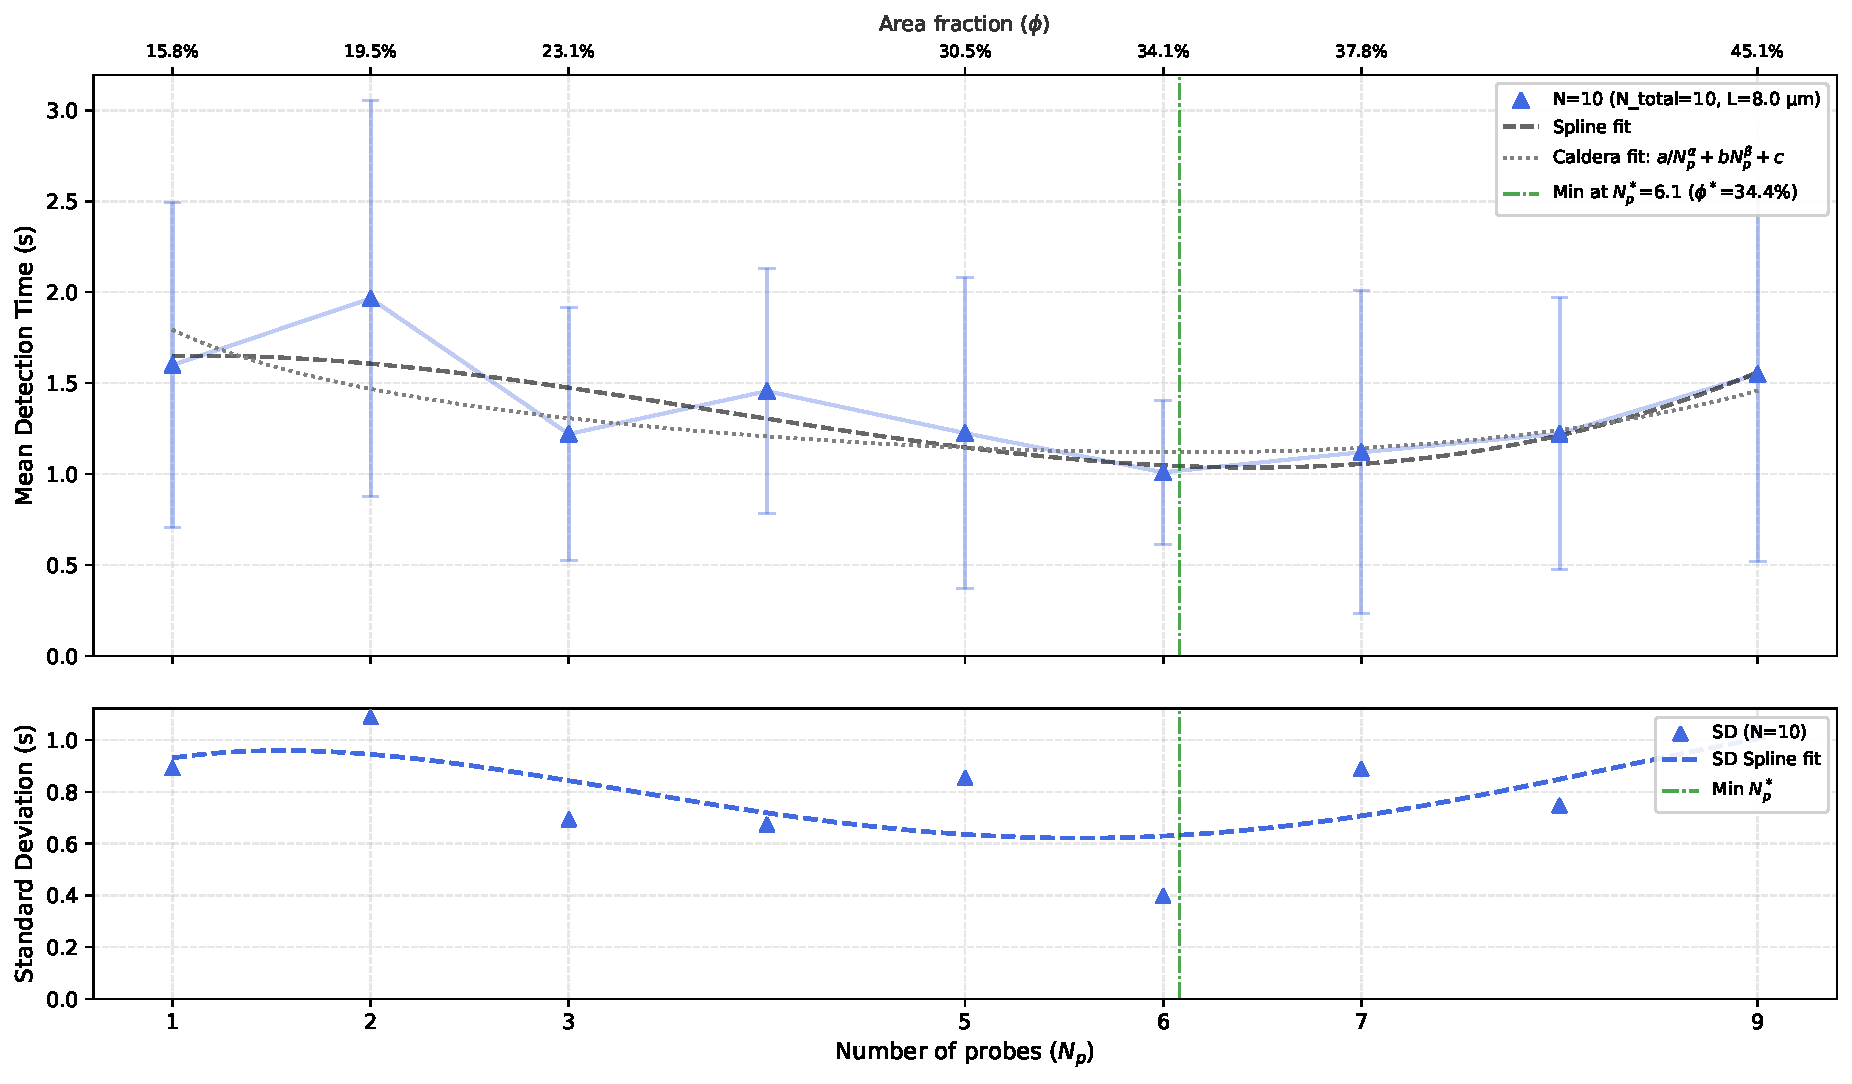
\includegraphics[width = 0.95\linewidth]{figures/caldera_individual_N_10.pdf}
    \caption{Mean first-passage detection time $\langle T \rangle$ (top) and its standard deviation (bottom) as a function of probe number $N_p$ (bottom axis) and area fraction $\phi$ (top axis) for the $N_\text{total} = 10$ system ($L = $ \SI{8.0}{\micro \meter}). The dotted curve is the caldera fit of Equation \ref{eq:3.6}; the dashed curve is the descriptive spline; the vertical dash-dot line marks the fitted optimum, $N_p = 6.1$ ($\phi \approx$ \SI{34.4}{\percent}).}
    \label{fig:Caldera10}
\end{figure}

\textbf{Figure~\ref{fig:Caldera10}} ($N_\text{total} = 10$) shows nine discrete probe counts available ($N_p = 1$ through $N_p = 9$), this is the coarsest-sampled system in the sweep, and it shows the noisiest curve of the six where its $\langle T \rangle$ rises from $N_p = 1$ to a local peak at $N_p = 2$ before beginning its overall decline, a non-monotonicity not seen in any larger system and consistent with run-to-run scatter dominating the signal at this system size. The minimum sits in a shallow, broad caldera spanning roughly $N_p = 5$--7 ($\phi \approx 30$--38\%), where the caldera fit and the descriptive spline agree closely, before both curves turn upward toward $N_p = 9$. The standard-deviation panel echoes this shape, narrowing to its tightest point near the fitted optimum and widening sharply at both the $N_p = 2$ and $N_p = 9$ extremes, with error bars at every point large enough to overlap several neighboring $N_p$ values.

\begin{figure}[htbp]
    \centering
    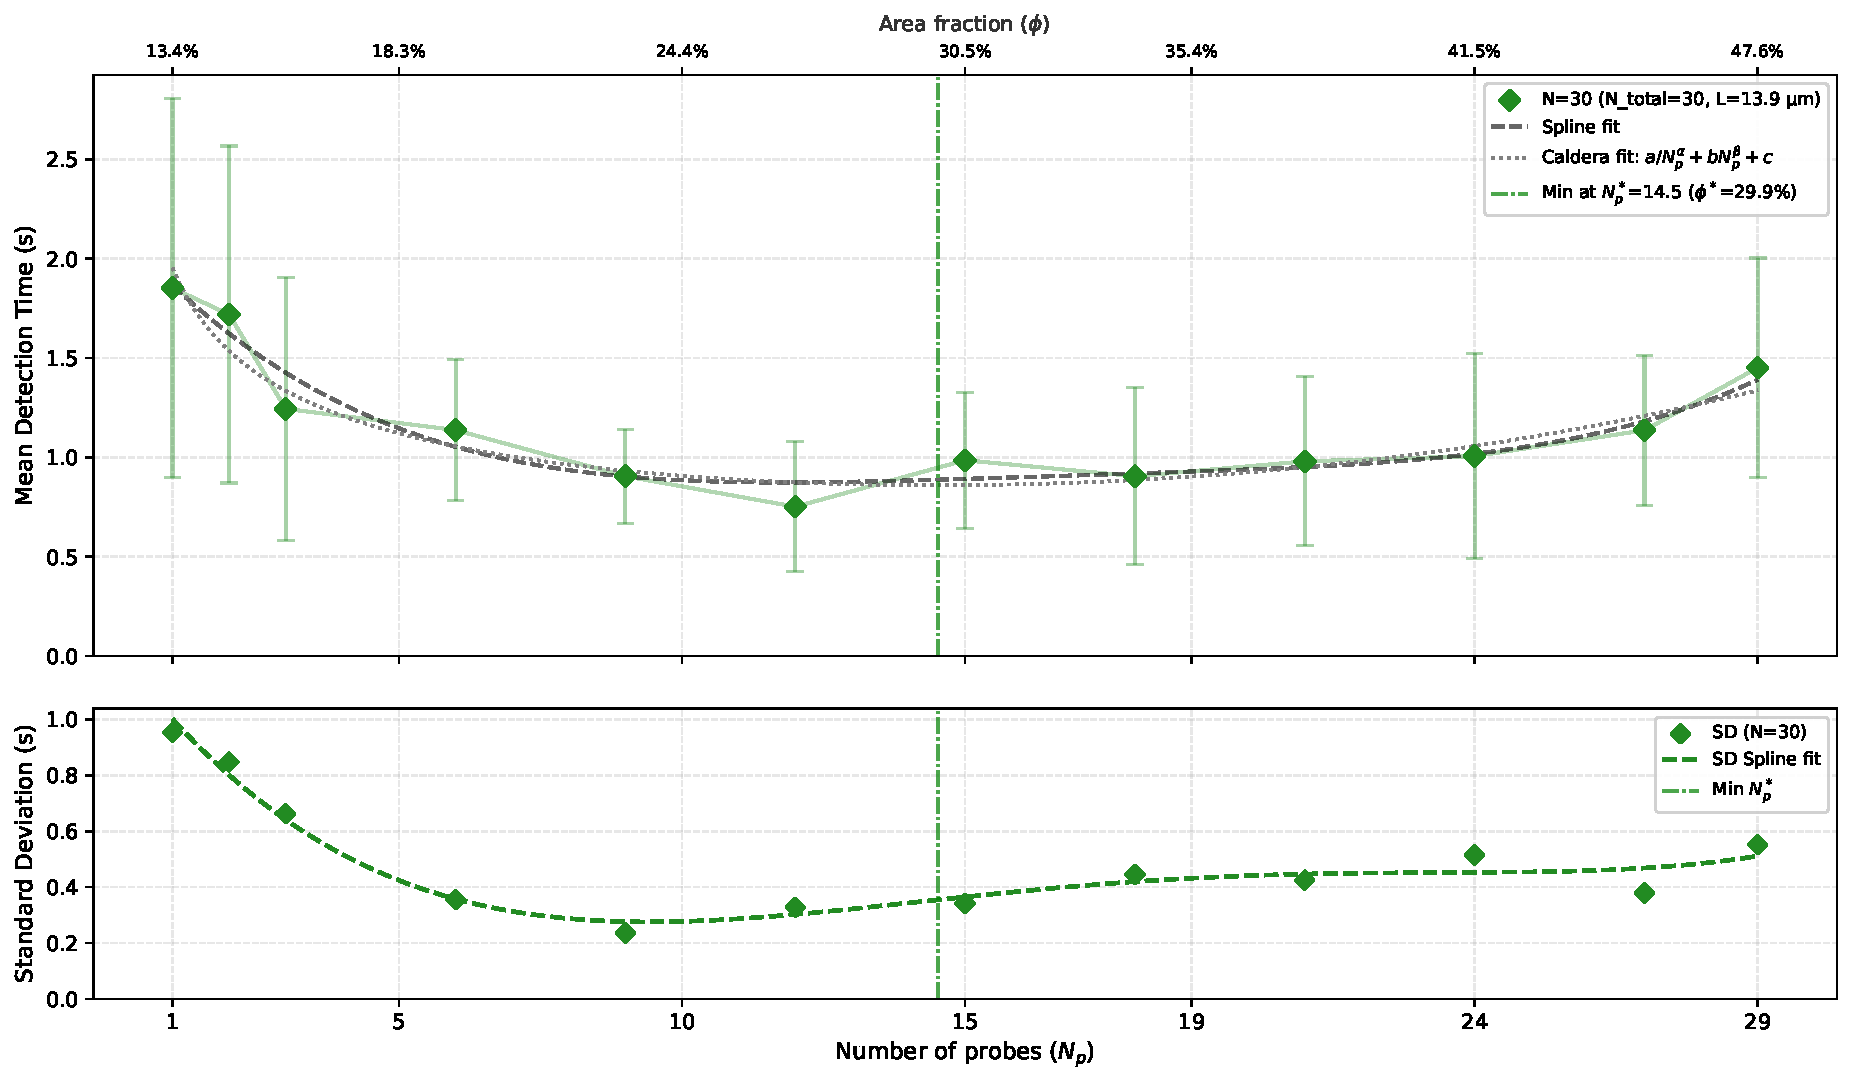
\includegraphics[width = 0.95\linewidth]{figures/caldera_individual_N_30.pdf}
    \caption{Mean first-passage detection time $\langle T \rangle$ (top) and its standard deviation (bottom) as a function of probe number $N_p$ (bottom axis) and area fraction $\phi$ (top axis) for the $N_\text{total} = 30$ system ($L = $ \SI{13.9}{\micro \meter}). The dotted curve is the caldera fit of Equation \ref{eq:3.6}; the dashed curve is the descriptive spline; the vertical dash-dot line marks the fitted optimum, $N_p = 14.5$ ($\phi \approx$ \SI{29.9}{\percent}).}
    \label{fig:Caldera30}
\end{figure}

\textbf{Figure~\ref{fig:Caldera30}} ($N_\text{total} = 30$) shows twelve sampled $N_p$ values, this curve is visibly smoother than the $N_\text{total} = 10$ case where its $\langle T \rangle$ falls steadily from its highest value at $N_p = 1$ to a floor spanning roughly $N_p = 9$--15 ($\phi \approx 23$--30\%), then rises gently but steadily out to $N_p = 29$. The caldera fit and the spline lie almost on top of one another across the entire sampled range, and the error bars while still substantial at $N_p = 1$--2, contract markedly once $N_p$ exceeds about 5. The standard-deviation panel reaches its minimum in the same $N_p$ window as $\langle T \rangle$'s floor and then climbs slowly and almost linearly through the rest of the sweep, without the sharp late upturn seen in the larger system below.

\begin{figure}[htbp]
    \centering
    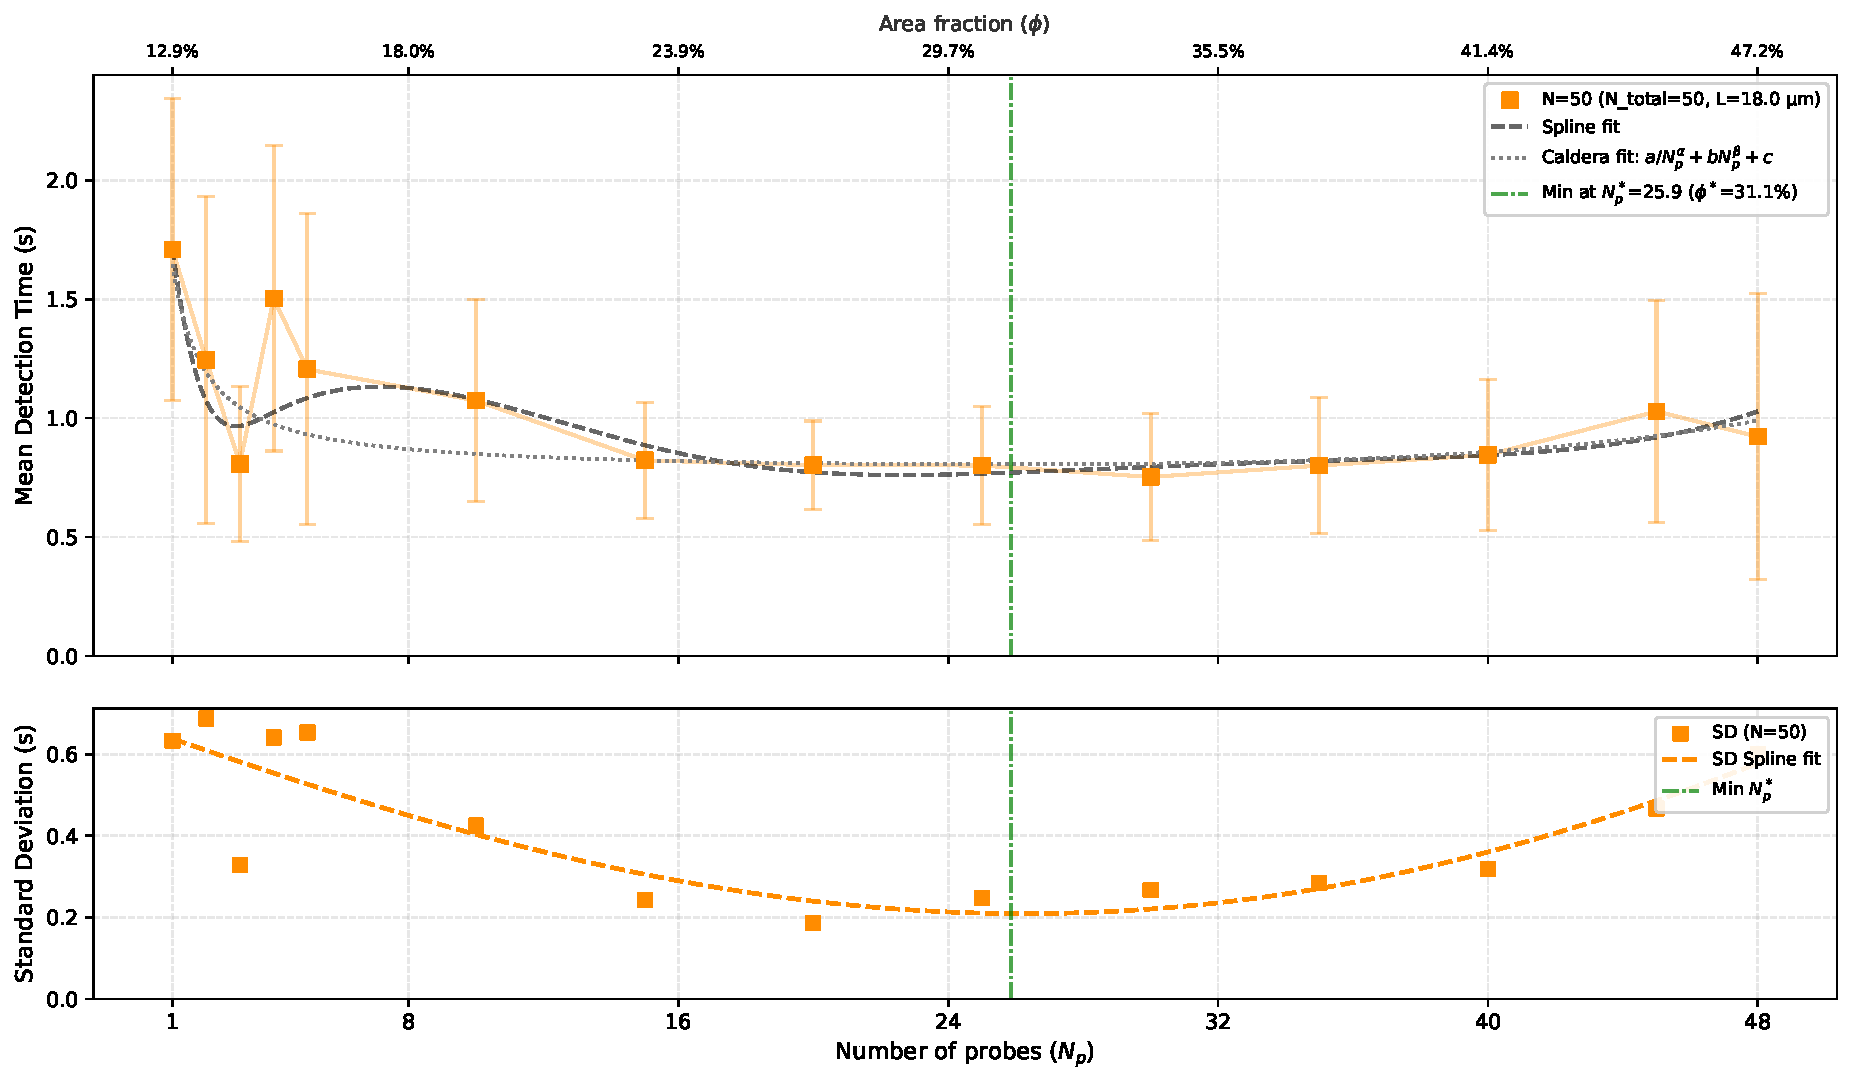
\includegraphics[width = 0.95\linewidth]{figures/caldera_individual_N_50.pdf}
    \caption{Mean first-passage detection time $\langle T \rangle$ (top) and its standard deviation (bottom) as a function of probe number $N_p$ (bottom axis) and area fraction $\phi$ (top axis) for the $N_\text{total} = 50$ system ($L = $ \SI{18.0}{\micro \meter}). The dotted curve is the caldera fit of Equation \ref{eq:3.6}; the dashed curve is the descriptive spline; the vertical dash-dot line marks the fitted optimum, $N_p = 25.9$ ($\phi \approx$ \SI{31.1}{\percent}).}
    \label{fig:Caldera50}
\end{figure}

\textbf{Figure~\ref{fig:Caldera50}} ($N_\text{total} = 50$) shows a pronounced early spike where its $\langle T \rangle$ at $N_p = 4$ briefly exceeds the values at $N_p = 2$, a small non-monotonicity similar in character (though milder than) the one seen at $N_\text{total} = 10$, before the curve settles into a long, flat floor extending from roughly $N_p = 16$ to $N_p = 32$ ($\phi \approx 24$--35\%). The caldera fit tracks the spline closely through this flat region and diverges only mildly on the crowded side, where the fit rises somewhat more gently than the raw points suggest. The standard deviation is largest and most erratic over the first few, most dilute points, drops to its lowest and most stable values across the same flat floor as $\langle T \rangle$, and turns upward again past $N_p \approx 32$, though this rise is modest compared to the sharper upturn seen in the three largest systems.

\begin{figure}[htbp]
    \centering
    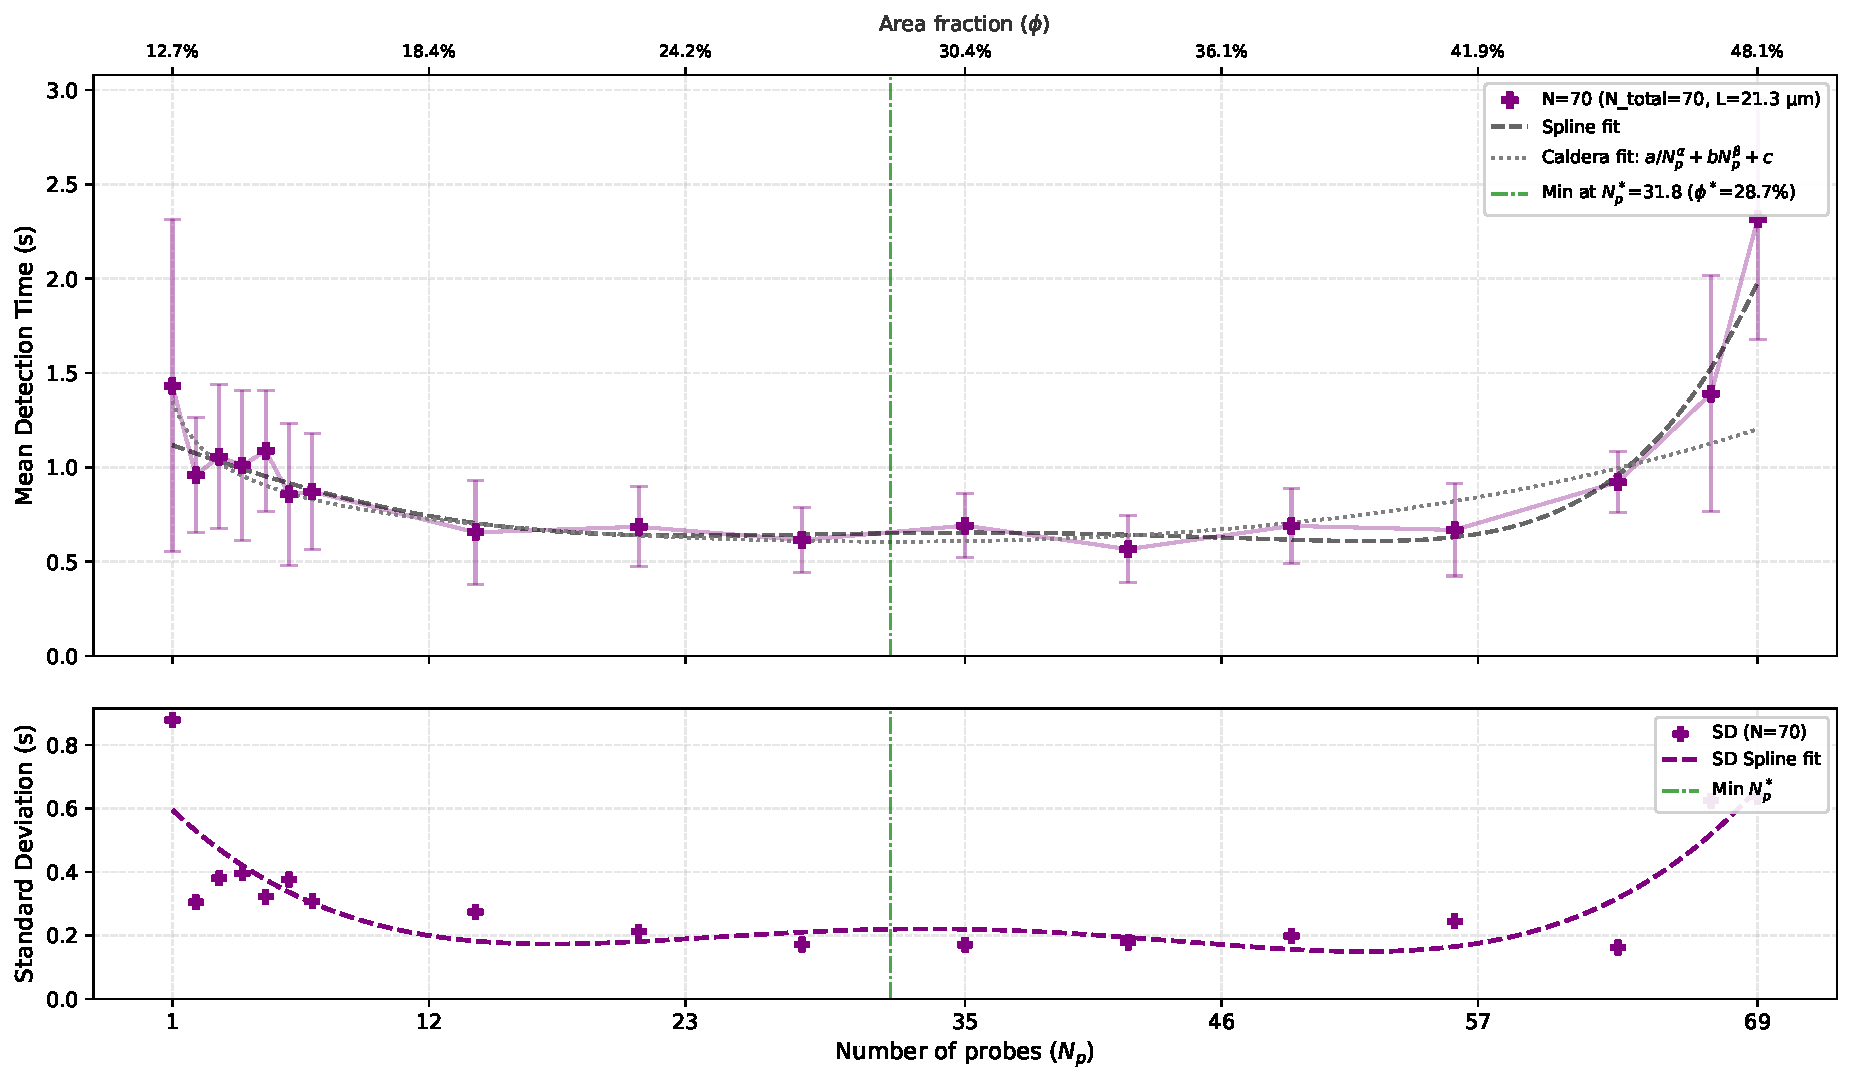
\includegraphics[width = 0.95\linewidth]{figures/caldera_individual_N_70.pdf}
    \caption{Mean first-passage detection time $\langle T \rangle$ (top) and its standard deviation (bottom) as a function of probe number $N_p$ (bottom axis) and area fraction $\phi$ (top axis) for the $N_\text{total} = 70$ system ($L = $ \SI{21.3}{\micro \meter}). The dotted curve is the caldera fit of Equation \ref{eq:3.6}; the dashed curve is the descriptive spline; the vertical dash-dot line marks the fitted optimum, $N_p = 31.8$ ($\phi \approx$ \SI{28.7}{\percent}).}
    \label{fig:Caldera70}
\end{figure}

\textbf{Figure~\ref{fig:Caldera70}} ($N_\text{total} = 70$) is the first system in the sweep where the caldera shape becomes visually ambiguous rather than merely fitted. Its $\langle T \rangle$ drops sharply over the first dozen or so probes, settles into a long, low, comparatively flat plateau from roughly $N_p = 12$ to $N_p =46$ ($\phi\approx 18$--42\%), and then rises sharply and clearly over the final several points, with the last two or three sampled conditions visibly separated from the plateau even accounting for their error bars. The standard deviation is lowest and most tightly clustered across the same wide plateau and increases sharply in step with $\langle T \rangle$ at the crowded edge, more than doubling between the floor and the final sampled point. This is the first system size at which the crowded-side rise is clearly resolved above the noise floor rather than merely suggested by the fit.

\begin{figure}[H]
    \centering
    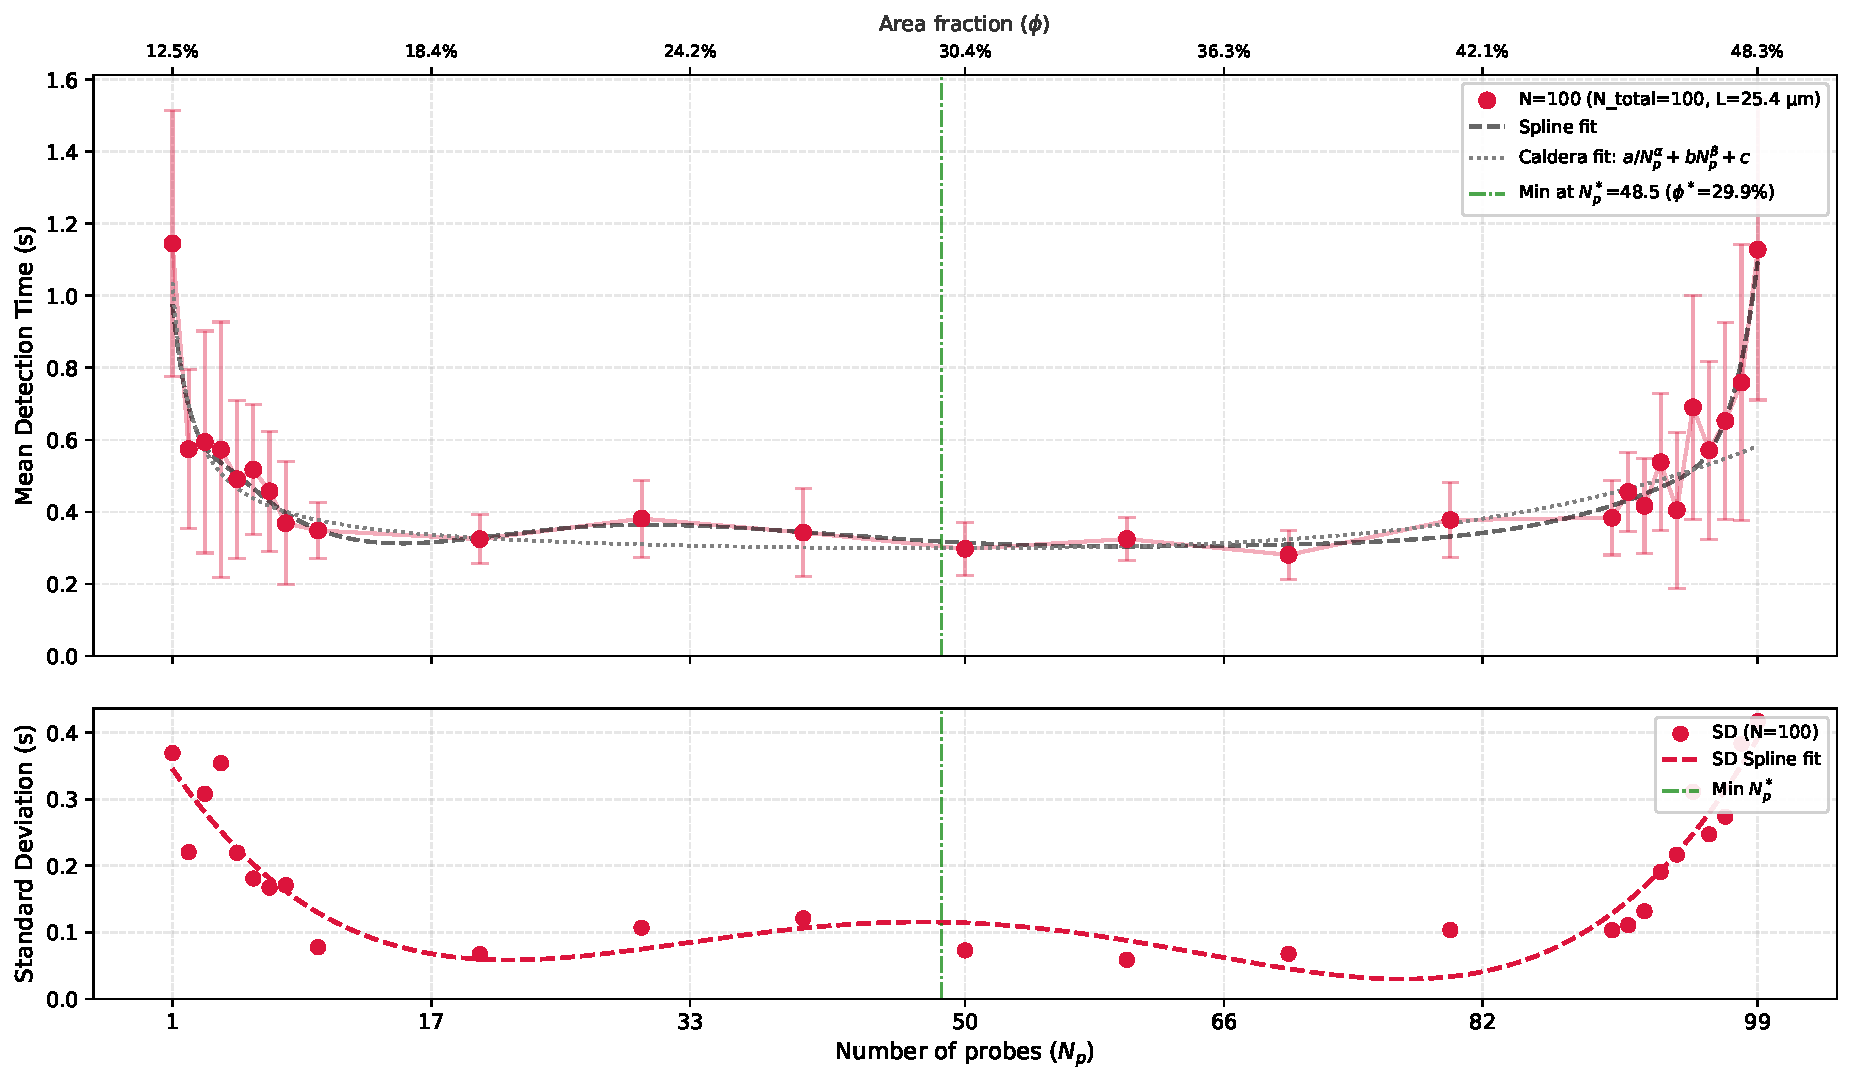
\includegraphics[width = 0.95\linewidth]{figures/caldera_individual_N_100.pdf}
    \caption{Mean first-passage detection time $\langle T \rangle$ (top) and its standard deviation (bottom) as a function of probe number $N_p$ (bottom axis) and area fraction $\phi$ (top axis) for the $N_\text{total} = 100$ system ($L = $ \SI{25.4}{\micro \meter}). The dotted curve is the caldera fit of Equation \ref{eq:3.6}; the dashed curve is the descriptive spline; the vertical dash-dot line marks the fitted optimum, $N_p = 48.5$ ($\phi \approx$ \SI{29.9}{\percent}).}
    \label{fig:Caldera100}
\end{figure}

\textbf{Figure~\ref{fig:Caldera100}} ($N_\text{total} = 100$) shows twenty sampled $N_p$ values, and this is one of the two most finely resolved systems in the sweep, and its caldera shape is the cleanest of the six. Its $\langle T \rangle$ falls from just over 1\,s at $N_p=1$ to a floor near 0.3\,s that is sustained, essentially flat, from roughly $N_p =17$ to $N_p = 66$ ($\phi \approx 18$--36\%), before rising steeply over the last quarter of the sweep to end close to its starting value near $N_p = 99$. The standard deviation mirrors this shape almost exactly, falling 0.1\,s across the plateau and climbing back above 0.3\,s at the crowded edge. The caldera fit and spline are nearly indistinguishable thorugh the plateau and separate only slightly on the crowded flank, where the raw points show somewhat more scatter than the smooth fit implies.

\begin{figure}[H]
    \centering
    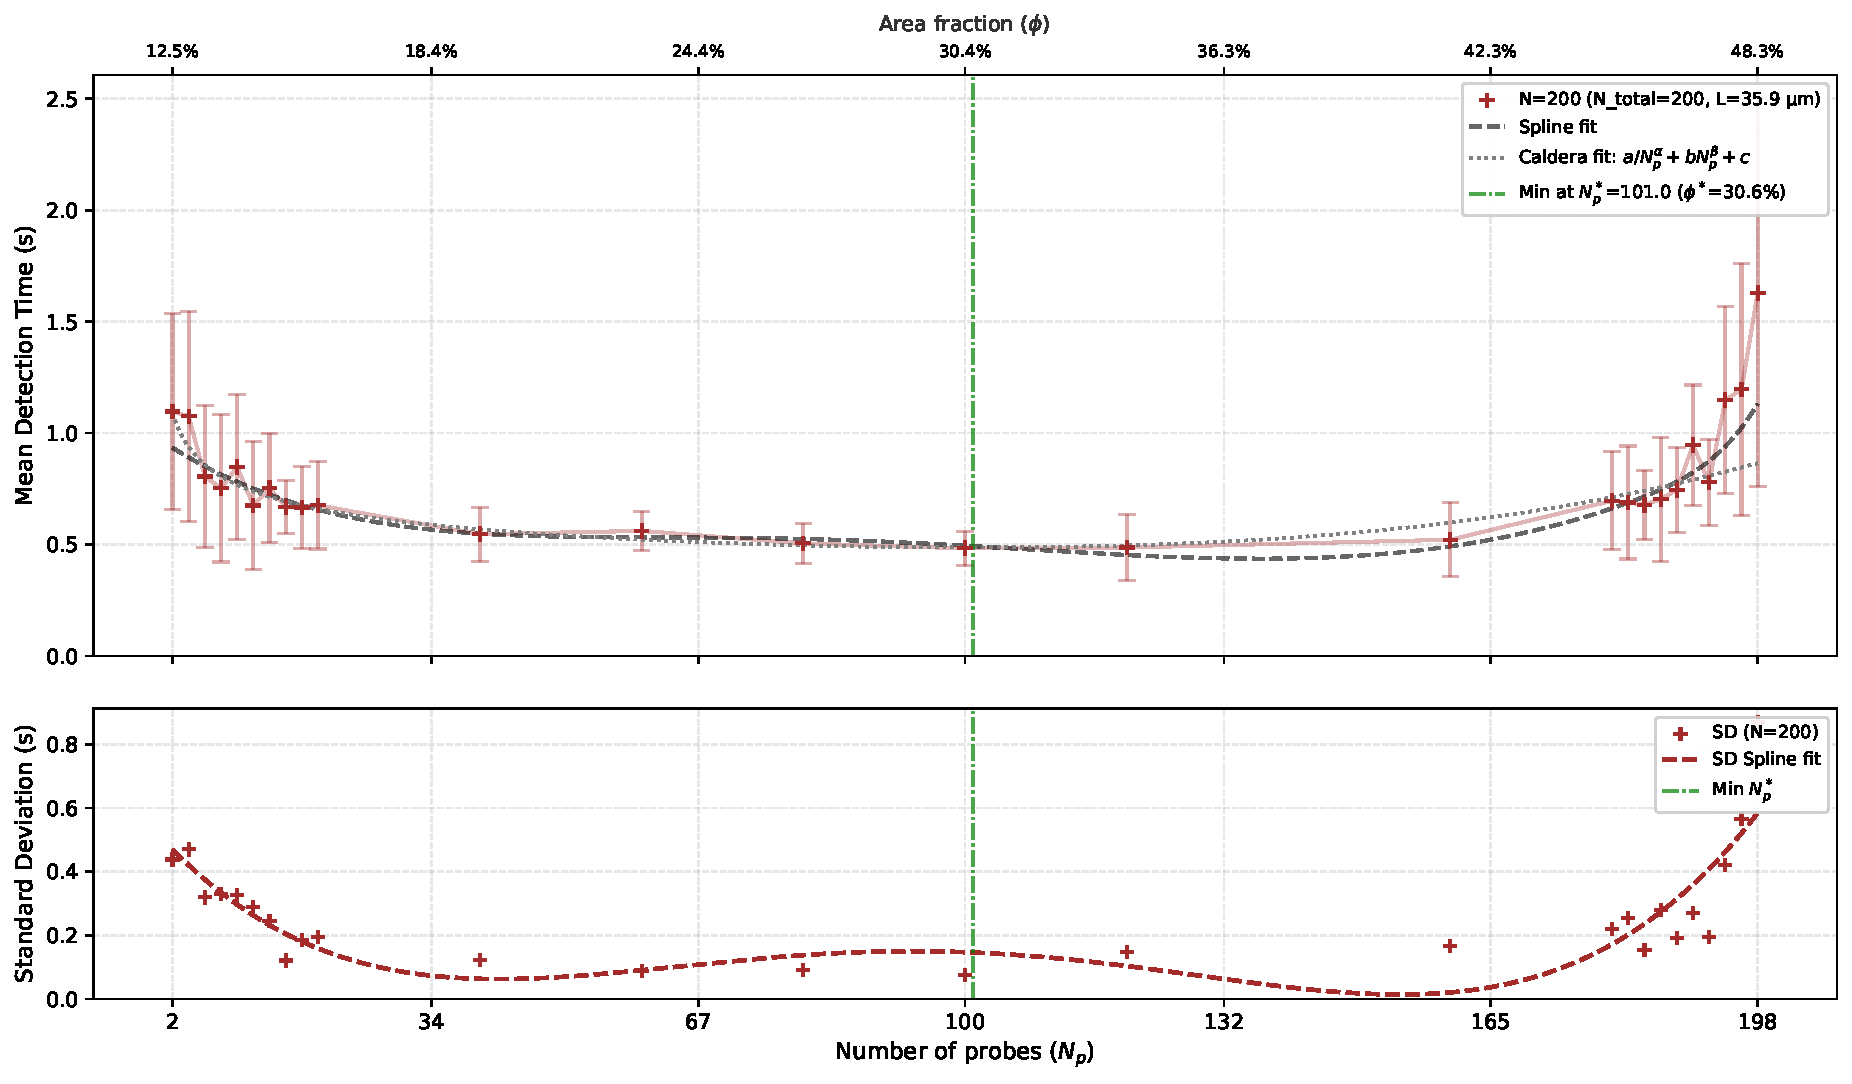
\includegraphics[width = 0.95\linewidth]{figures/caldera_individual_N_200.pdf}
    \caption{Mean first-passage detection time $\langle T \rangle$ (top) and its standard deviation (bottom) as a function of probe number $N_p$ (bottom axis) and area fraction $\phi$ (top axis) for the $N_\text{total} = 200$ system ($L = $ \SI{35.9}{\micro \meter}). The dotted curve is the caldera fit of Equation \ref{eq:3.6}; the dashed curve is the descriptive spline; the vertical dash-dot line marks the fitted optimum, $N_p = 101.0$ ($\phi \approx$ \SI{30.6}{\percent}).}
    \label{fig:Caldera200}
\end{figure}

\textbf{Figure~\ref{fig:Caldera200}} ($N_\text{total} = 200$) shows the largest and most finely sampled system, this plot shows the widest and flattest floor of the six, extending from roughly $N_p = 34$ to $N_p = 132$ ($\phi \approx 18$--42\%) at a level near 0.5\,s which is noticeable higher than the $N_\text{total}=100$ floor, the reversal discussed in Section~\ref{sec:4.10}. The rise at the crowded edge is the steepest of any system in absolute terms, with the final few moments climbing past 1.5--2.5\,s and carrying the widest error bars in the entire sweep. The standard-deviation panel is correspondingly the most dramatic where it sits below 0.2\,s for the majority of the sampled range and rises sharply, almost vertically, over the last five or six points, indicating that both the typical detection time and its run-to-run variability degrade together once probe density passes roughly $\phi \approx 42$--48\%.

\section{Locating the Optimum: The Caldera Fit}
\label{sec:4.2}

Fitting equation~\ref{eq:3.6} to each system's $N_p, \langle T \rangle$ data locates a well-defined optimum in every case (Figures \ref{fig:Caldera10}--\ref{fig:Caldera200}, dotted curves). The fitted optimal probe number $N_p^*$ and corresponding area fraction $\phi^*$ for each system are summarized in Table~\ref{tab:caldera-optima}

% \begin{table}[htbp]
%     \centering
%     \caption{Fitted caldera optimum probe number and area fraction per system size.}
%     \begin{tabular}{ccc}
%     \hline   
%         $N_\text{total}$ & $N_p^*$ & $\phi^*$ \\
%     \hline     
%          10 & 6.1 & 34.4  \\
%          30 & 14.5 & 29.9  \\
%          50 & 25.9 & 31.1  \\
%          70 & 31.8 & 28.7  \\
%          100 & 48.5 & 29.9  \\
%          200 & 101.0 & 30.6  \\
%     \hline     
%     \end{tabular}
%     \label{tab:caldera-optima}
% \end{table}

\begin{table}[htbp]
\centering
\caption{Fitted caldera optimum probe number and area fraction per system size.}
\begin{tabular}{ccccccc}
\hline
\textbf{N$_\text{total}$} & \textbf{10} & \textbf{30} & \textbf{50} & \textbf{70} & \textbf{100} & \textbf{200} \\ \hline
\textbf{$N^*_p$}          & 6.1         & 14.5        & 25.9        & 31.8        & 48.5         & 101.0        \\
\textbf{$\phi^*$}         & 34.4        & 29.9        & 31.1        & 28.7        & 29.9         & 30.6         \\ \hline
\end{tabular}
\label{tab:caldera-optima}
\end{table}

Excluding $N_\text{total} = 10$, the fitted $\phi^*$ clusters tightly between 28.7\% and 31.1\% with a mean of $\approx 30.1\%$ despite the tenfold range in absolute system size from $N_\text{total} = 30$ to 200. The $N_\text{total} = 10$ system is a mild outlier at $\phi^* = 34.4\%$, a departure addressed directly in Section~\ref{sec:4.7}. In every system, the caldera fit (dotted) and the descriptive spline (dashed) track each other closely near the minimum, with the closest agreement in the $N_\text{total} = 30$, 50, 70, and 100 systems and the widest separation in the $N_\text{total} = 10$ system, where only nine discrete $N_p$ values are available to constrain the fit. Read together with the per-figure descriptions above, the fitted optimum consistently lands inside each system's visually flattest region of $\langle T \rangle$ rather than at an isolated point, which is the qualitative check that the two-term model of Equation~\ref{eq:3.6} is capturing a genuine caldera rather than over-fitting to a single low-noise data point.

\begin{figure}[htbp]
    \centering
    \includegraphics[width = 0.95\linewidth]{figures/Fig5_floor_summary.pdf}
    \caption{Floor-vs-system detection of mean detection time $\langle T \rangle$ and the Standard deviation time plotted against all the system size showing non-monotonic relationship of minimum detection with system size.}
    \label{fig:floorvssystem}
\end{figure}

Having identified the floor detection time for each system, Figure~\ref{fig:floorvssystem} compares these floor values directly across system sizes. The top panel shows the floor mean detection time $\langle T \rangle$, and the bottom panel shows its associated standard deviation, both plotted against $N_\text{total}$. The floor value decreases from $N=10$ through $N=100$, but then rises again at $N=200$, which indicates that the floor detection time is non-monotonic with system size rather than continuing to improve as the system grows. This suggests that increasing the overall system size does not uniformly improve the best achievable detection time once probe density is already optimized; beyond a certain scale (here, between $N=100$ and $N=200$), enlarging the system appears to work against detection efficiency at the floor, even though the same range of area fractions is sampled in both cases. A plausible explanation is that fixing the area fraction across differently sized systems does not fix the absolute length scales of the search domain which means a larger box at the same $\phi$ still requires probes and targets to cover proportionally larger physical distances between collisions, which can offset the benefit of having more probes available. The standard deviation panel shows the same qualitative trend, with the lowest run-to-run variability also occurring near $N=100$, suggesting this system size sits closest to an overall efficient and consistent detection regime within the range studied.

\section{Variance and Reliability Across the Search}
\label{sec:4.3}

\begin{figure}[htbp]
    \centering
    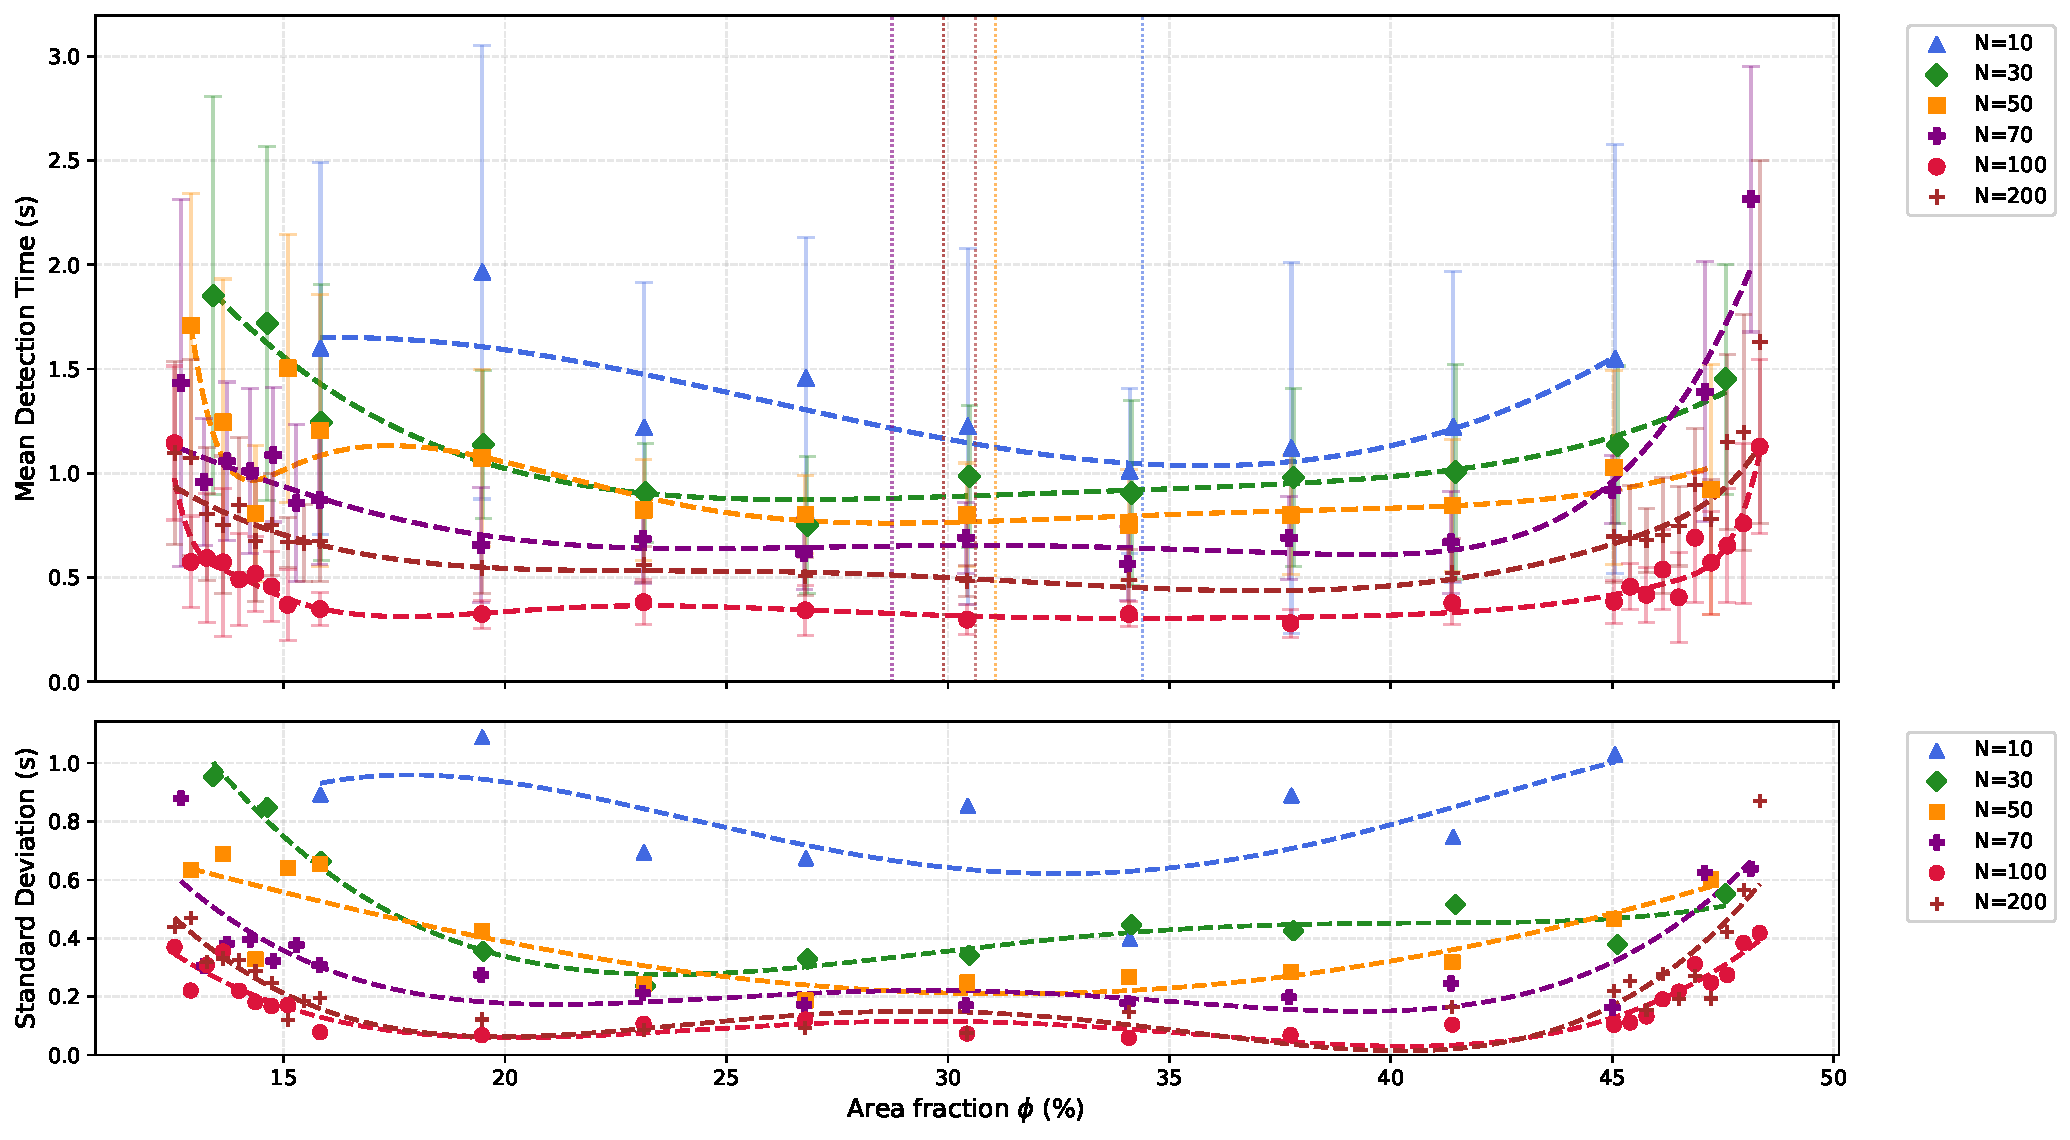
\includegraphics[width = 0.95\linewidth]{figures/caldera_overlay_phi.pdf}
    \caption{Overlay of mean first-passage detection time (top) and standard deviation (bottom) versus area fraction $\phi$ for all six system sizes ($N_\text{total} = 10,30,50,70, 100,200$), each with its own descriptive spline fit, allowing the caldera minimum and the width of the crowding onset to be compared directly across system scales on a common $\phi$ axis.}
    \label{fig:OverlayCaldera}
\end{figure}

\textbf{Figure~\ref{fig:OverlayCaldera}} plots all six systems on a common area-fraction axis, rather than on their individual $N_P$ axes, makes two features visible that are hard to see in Figures~\ref{fig:4.1}--\ref{fig:4.6} taken one at a time. First, the six curves are stacked in the same order in both panels throughout the sampled range. $N_\text{total} = 10$ sits highest in both $\langle T \rangle$ and standard deviation at almost every $\phi$, while $N_\text{total} =100$ sits lowest, with $N_\text{total} =200$ tucked just above it rather than below it, reproducing the floor-value reversal noted in Section~\ref{sec:4.1}. Second, the minima of all six splines cluseter in a visibly narrow band of the shared $\phi$ axis, roughly between 25\% and 35\%, even though the curves are otherwise offset from one another by as much as a factor of two to three in absolute $\langle T \rangle$. The overlay overlay shows that the same caldera structure seen in $\langle T \rangle$ appears independently in the standard deviation, for every system size where this is a non-trivial consistency check, since it means the caldera minimum in $\langle T \rangle$ is not merely a shift in central tendency accompanied by unchanged or worsening spread, this means that the search becomes both faster and more reproducible across independent seeds in the same $N_p$/$\phi$ window. Across the larger systems ($N_\text{total} = 70, 100, 200$), the standard deviation rises more steeply on the crowded (high-$N_p$) side of the caldera than it falls on the dilute side; for example, in the $N_\text{total} = 100$ system the standard deviation grows from roughly 0.1\,s near the floor to over 0.3\,s by $N_p =99$, a threefold increase, while the corresponding rise in $\langle T \rangle$ over the same range is comparatively more gradual. This asymmetric growth in variance, ahead of a comparably sharp rise in the mean, foreshadows the distributional broadening examined directly in Section~\ref{sec:4.5}.

\section{The Ergodic Product}
\label{sec:4.4}

The ergodic product $E = N_p \times \langle T \rangle$ tracks its linear sub-critical extrapolation closely at low $N_p$ in every system, by construction, and departs upward from that extrapolation as $N_p$ increases. The six individual plots  (Figures~\ref{fig:ErgodicProduct10}--\ref{fig:ErgodicProduct200}) and their cross-system overlay (Figure~\ref{fig:OverlayErgodicProduct}) are described in turn below.

\begin{figure}[htbp]
    \centering
    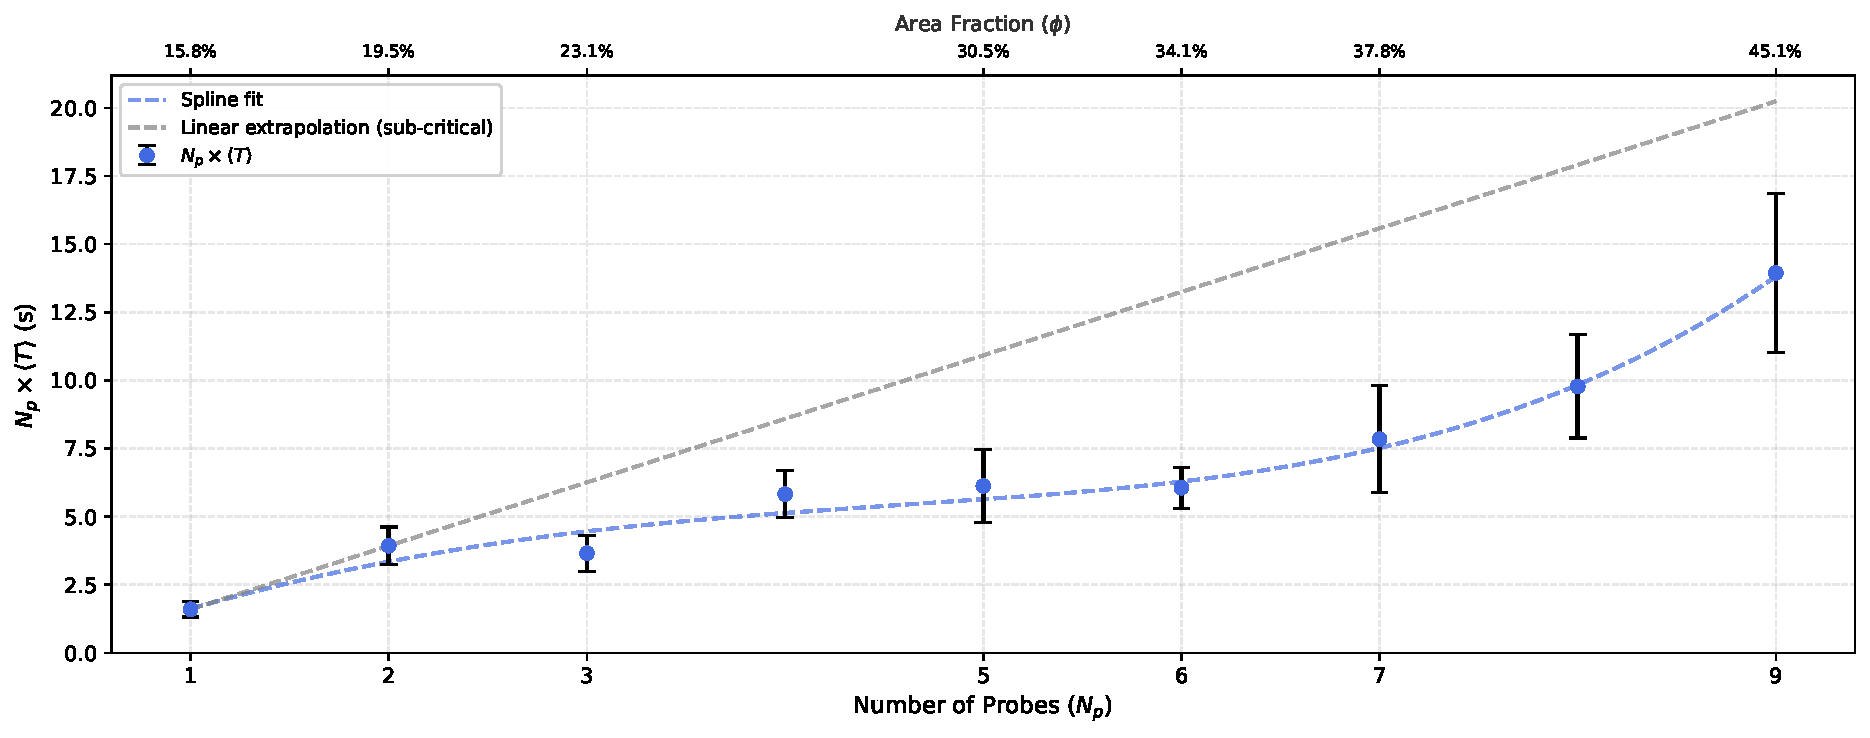
\includegraphics[width = 0.95\linewidth]{figures/ergodic_individual_N_10.pdf}
    \caption{Ergodic product $E = N_p\times \langle T\rangle$ versus $N_p$ and $\phi$ for the $N_\text{total} = 10$ system. The dashed line is a linear extrapolation of $E$ from the most dilute (sub-critical) points, representing the ideal, non-interacting-searcher expectation; the spline traces the actual measured values, and its upward departure from the extrapolation signals the onset of non-ergodic, crowding-influenced search.}
    \label{fig:ErgodicProduct10}
\end{figure}

\textbf{Figure~\ref{fig:ErgodicProduct10}} ($N_\text{total} = 10$) shows that $E$ tracks its sub-critical extrapolation reasonably well through the first four or five probe counts, but the departure that follows is gradual rather than sharp, and the error bars which are already wide in absolute $\langle T \rangle$ for this system (Figure~\ref{fig:Caldera10}) grows wide enough by $N_p = 7$--9 to overlap the extrapolation line itself. A departure is visually suggested by $N_p = 7$, but it cannot be called unambiguous given the size of the uncertainty at that point. 

\begin{figure}[htbp]
    \centering
    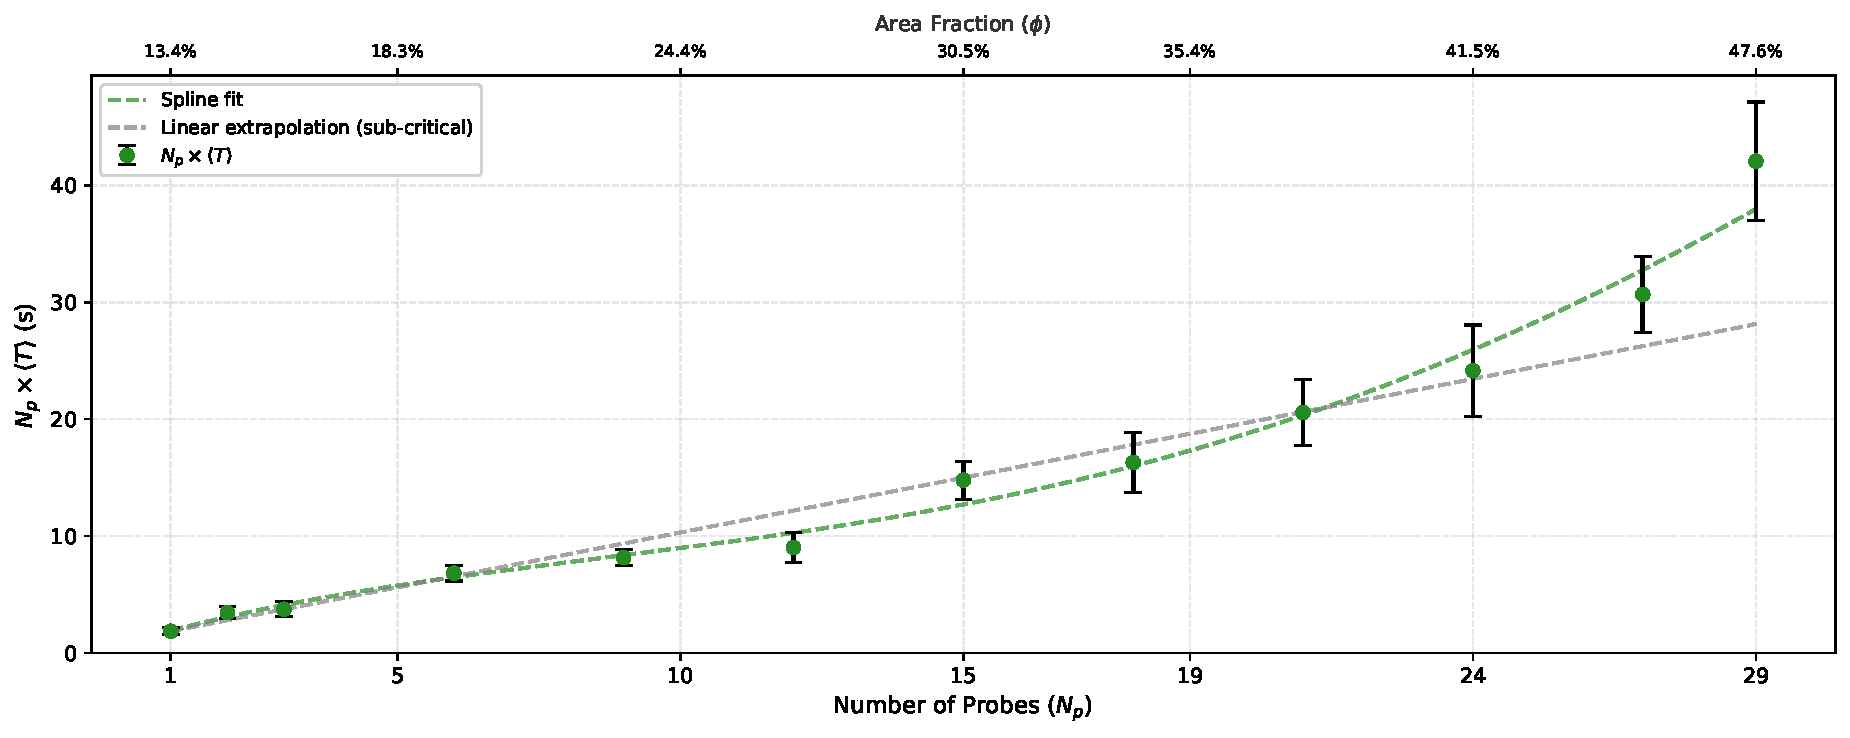
\includegraphics[width = 0.95\linewidth]{figures/ergodic_individual_N_30.pdf}
    \caption{Ergodic product $E = N_p\times \langle T\rangle$ versus $N_p$ and $\phi$ for the $N_\text{total} = 30$ system. The dashed line is a linear extrapolation of $E$ from the most dilute (sub-critical) points, representing the ideal, non-interacting-searcher expectation; the spline traces the actual measured values, and its upward departure from the extrapolation signals the onset of non-ergodic, crowding-influenced search.}
    \label{fig:ErgodicProduct30}
\end{figure}

\textbf{Figure~\ref{fig:ErgodicProduct30}} ($N_\text{total} = 30$) shows that $E$ follows its extrapolation closely and with tight error bars out to roughly $N_p = 19$, then separates visibly, if still gently, over the last three sampled points, reaching roughly 1.3--1.5$\times$ the extrapolated value by $N_\text{total} = 10$ system but remains modest in magnitude relative to the sharp separations seen in the larger systems below.

\begin{figure}[htbp]
    \centering
    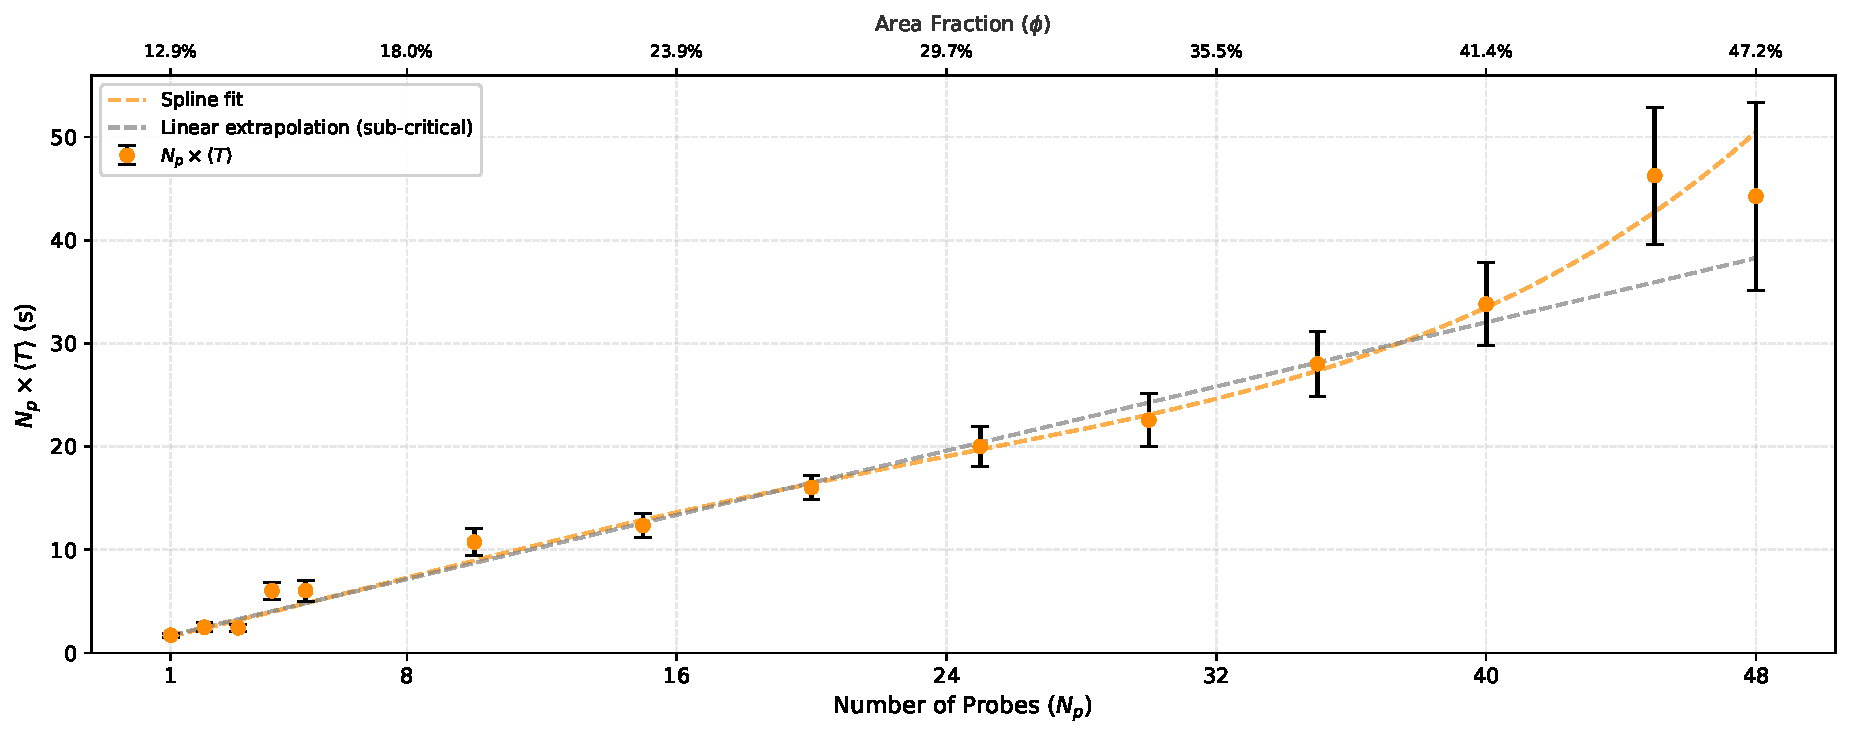
\includegraphics[width = 0.95\linewidth]{figures/ergodic_individual_N_50.pdf}
    \caption{Ergodic product $E = N_p\times \langle T\rangle$ versus $N_p$ and $\phi$ for the $N_\text{total} = 50$ system. The dashed line is a linear extrapolation of $E$ from the most dilute (sub-critical) points, representing the ideal, non-interacting-searcher expectation; the spline traces the actual measured values, and its upward departure from the extrapolation signals the onset of non-ergodic, crowding-influenced search.}
    \label{fig:ErgodicProduct50}
\end{figure}

\textbf{Figure~\ref{fig:ErgodicProduct50}} ($N_\text{total} = 50$) shows the measured $E$ and its extrapolation are nearly coincident through the first twenty-four probes, with small, tight error bars throughout this range. The departure appears only at the last two sampled points ($N_p =40$ and 48), where $E$ rises to roughly 1.3--1.5$\times$ the extrapolated values where the error bars at these two points are wider than elsewhere in the curve but still leave the departure visually distinguishable from the extrapolation line.

\begin{figure}[htbp]
    \centering
    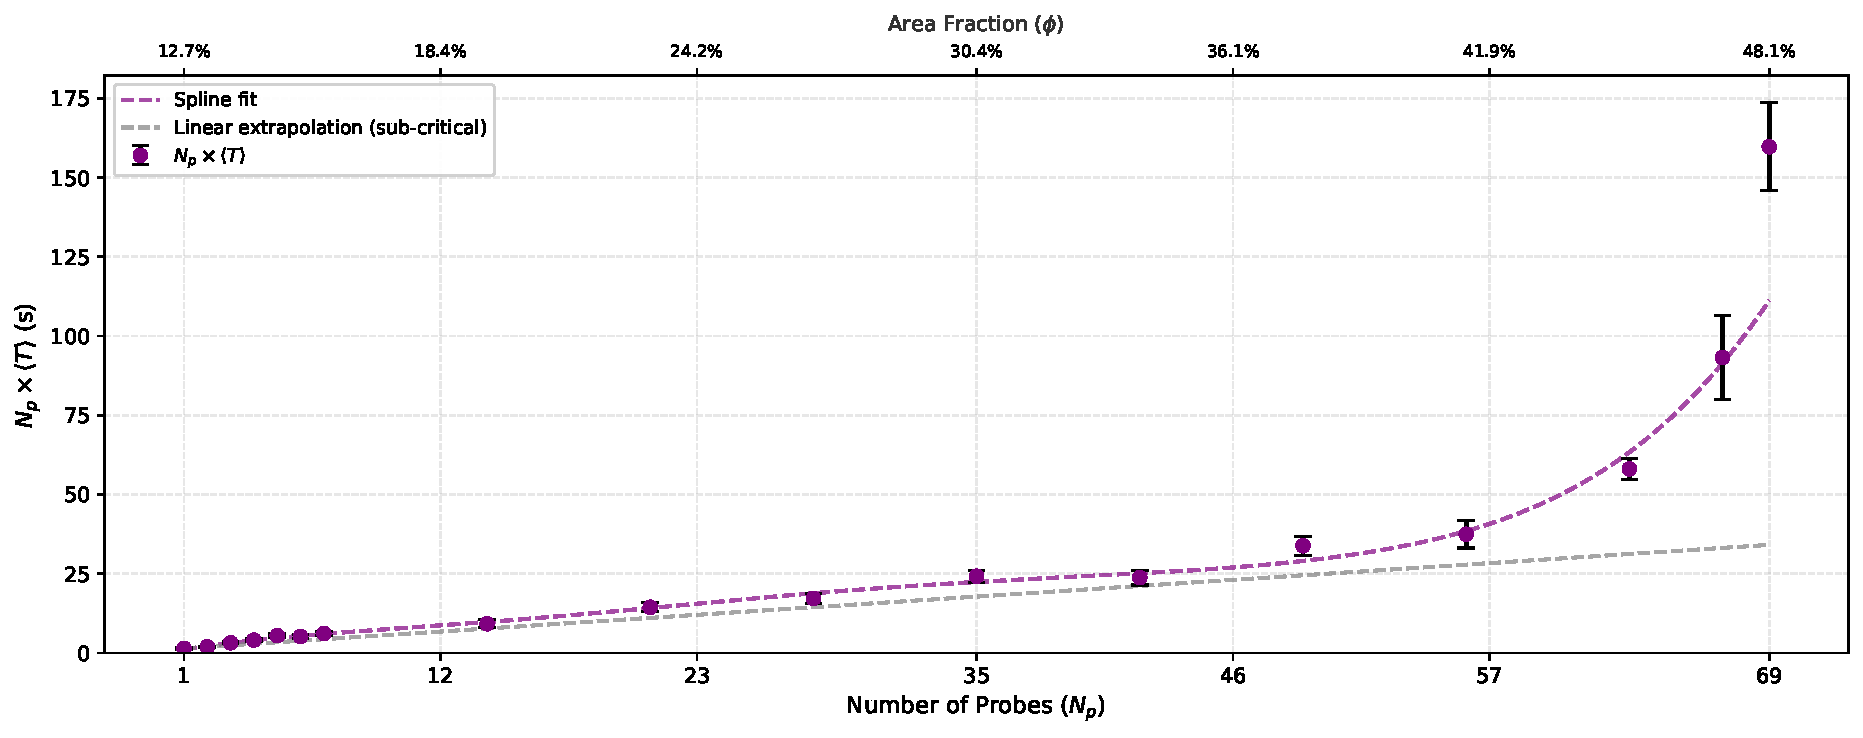
\includegraphics[width = 0.95\linewidth]{figures/ergodic_individual_N_70.pdf}
    \caption{Ergodic product $E = N_p\times \langle T\rangle$ versus $N_p$ and $\phi$ for the $N_\text{total} = 70$ system. The dashed line is a linear extrapolation of $E$ from the most dilute (sub-critical) points, representing the ideal, non-interacting-searcher expectation; the spline traces the actual measured values, and its upward departure from the extrapolation signals the onset of non-ergodic, crowding-influenced search.}
    \label{fig:ErgodicProduct70}
\end{figure}

\textbf{Figure~\ref{fig:ErgodicProduct70}} ($N_\text{total} = 70$) shows the first system where the departure is sharp and unambiguous. $E$ hugs its extrapolation almost exactly out to roughly $N_p = 46$, then bends away clearly, with error bars small enough relative to the separation that the last four or five points sit entirely above the extrapolation line rather than merely trending above it. By the final point ($N_p = 69$), the measured $E$ is roughly 1.5$\times$ its extrapolated value.

\begin{figure}[htbp]
    \centering
    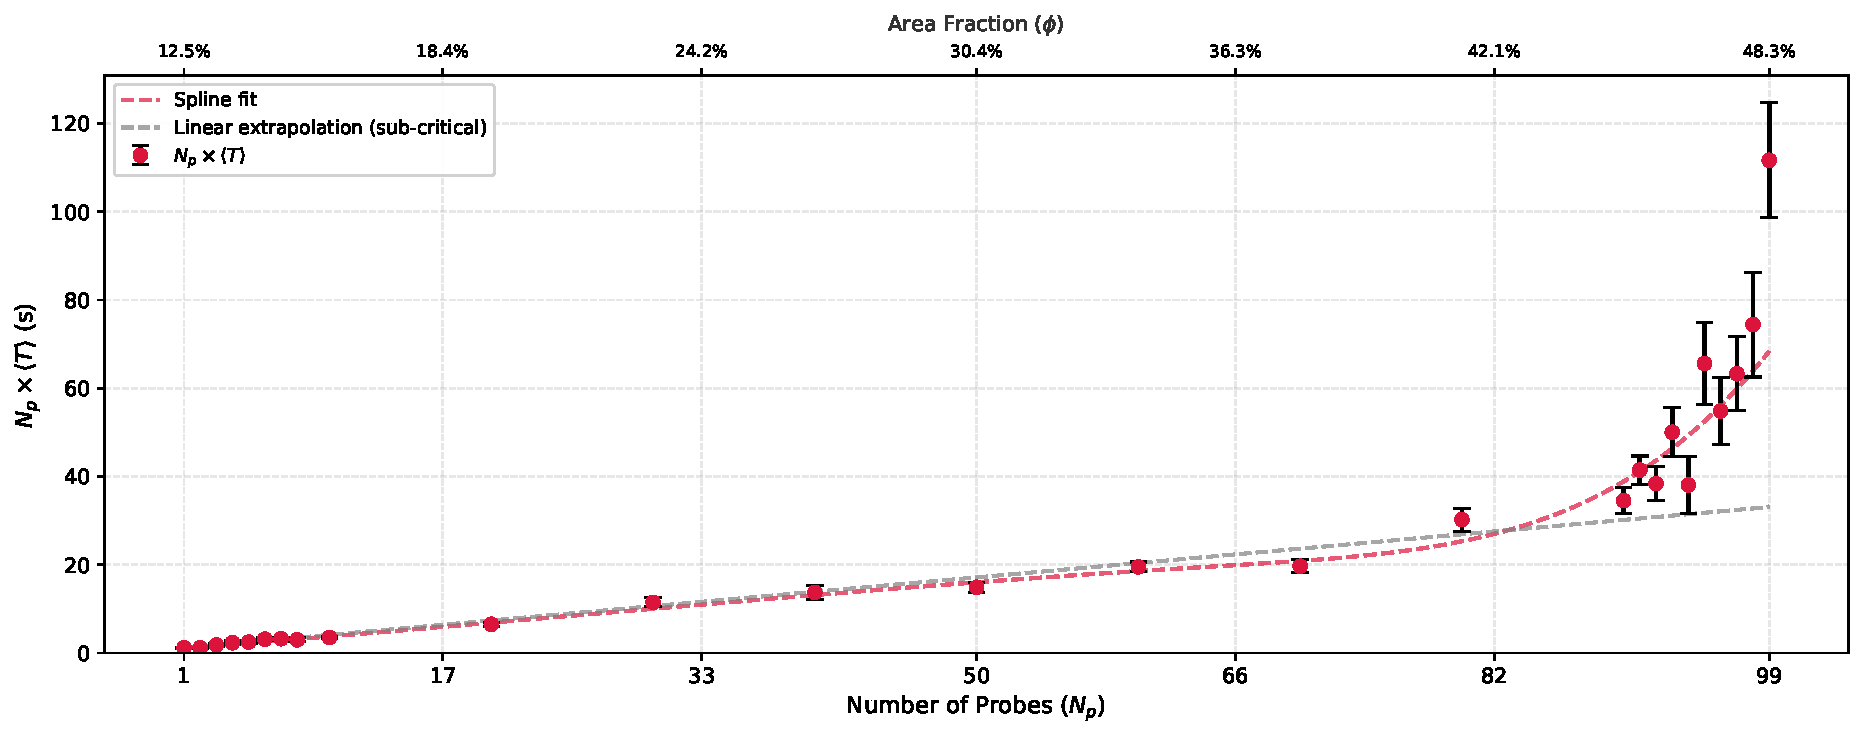
\includegraphics[width = 0.95\linewidth]{figures/ergodic_individual_N_100.pdf}
    \caption{Ergodic product $E = N_p\times \langle T\rangle$ versus $N_p$ and $\phi$ for the $N_\text{total} = 100$ system. The dashed line is a linear extrapolation of $E$ from the most dilute (sub-critical) points, representing the ideal, non-interacting-searcher expectation; the spline traces the actual measured values, and its upward departure from the extrapolation signals the onset of non-ergodic, crowding-influenced search.}
    \label{fig:ErgodicProduct100}
\end{figure}

\textbf{Figure~\ref{fig:ErgodicProduct100}} ($N_\text{total} = 100$) have twenty sampled points where this plot shows the departure most cleanly of any system. $E$ sits on its extrapolation, within tight error bars, through roughly $N_p = 66$, then visibly separates by  $N_p \approx 70$--82, and continues climbing steeply to end near 100--200\,s by $N_p = 99$, several multiples above the extrapolated value at that point. This departure is visible well before the corresponding upturn is unambiguous in $\langle T \rangle$ itself (Figure~\ref{fig:Caldera100}), a comparison developed in Section~\ref{sec:4.8}.

\begin{figure}[htbp]
    \centering
    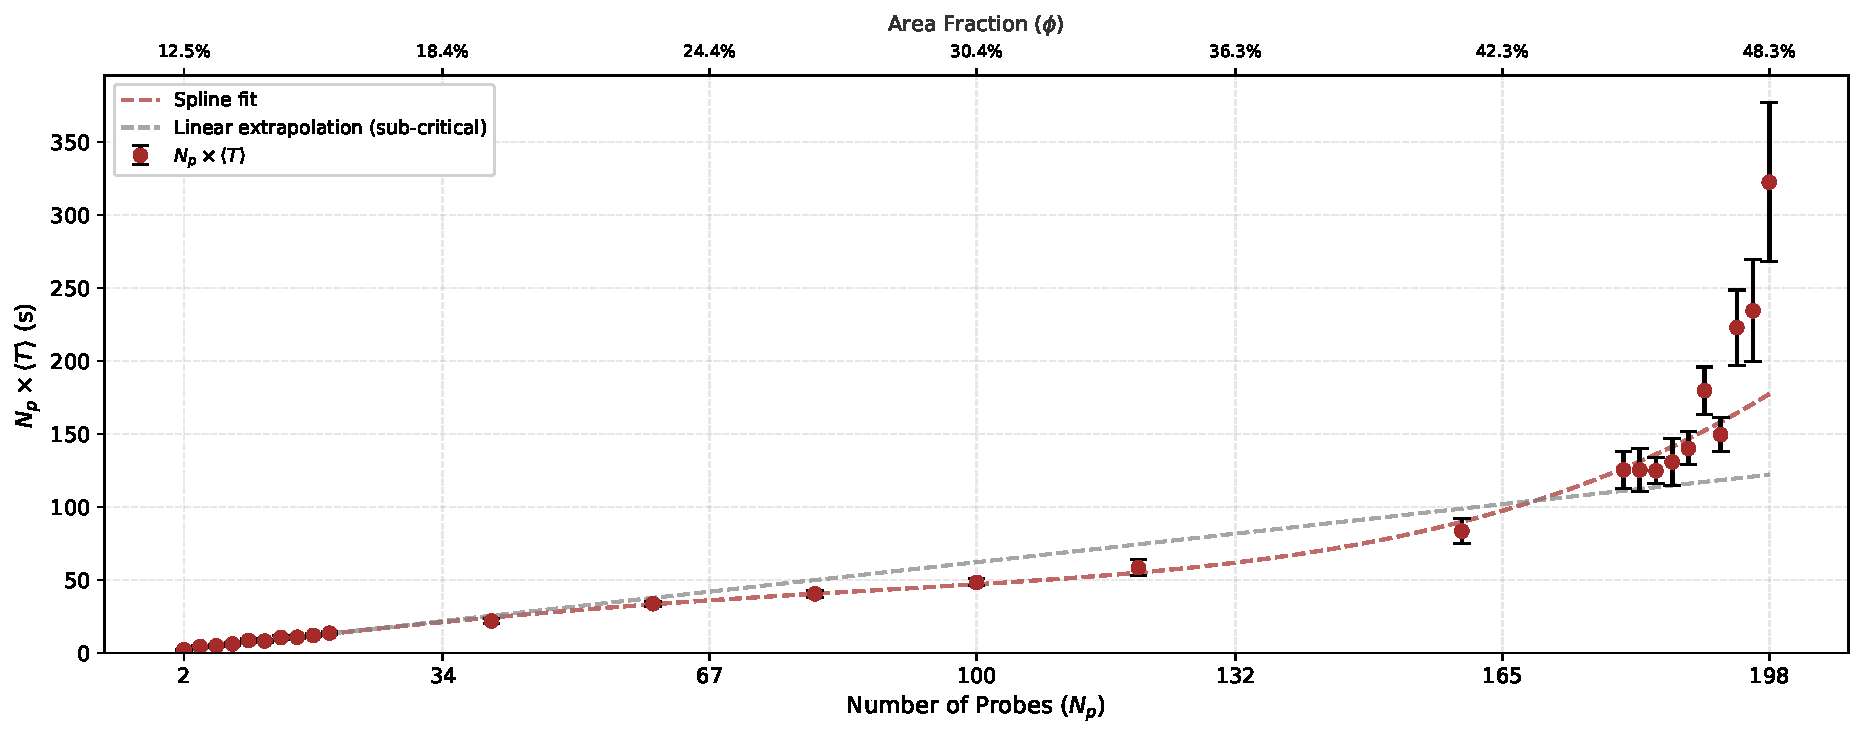
\includegraphics[width = 0.95\linewidth]{figures/ergodic_individual_N_200.pdf}
    \caption{Ergodic product $E = N_p\times \langle T\rangle$ versus $N_p$ and $\phi$ for the $N_\text{total} = 200$ system. The dashed line is a linear extrapolation of $E$ from the most dilute (sub-critical) points, representing the ideal, non-interacting-searcher expectation; the spline traces the actual measured values, and its upward departure from the extrapolation signals the onset of non-ergodic, crowding-influenced search.}
    \label{fig:ErgodicProduct200}
\end{figure}

\textbf{Figure~\ref{fig:ErgodicProduct200}} ($N_\text{total} = 200$) shows the dramatic absolute departure as the largest system. $E$ tracks its extrapolation closely out to roughly $N_p = 132$, then rises sharply, ending above 300\,s by the final sampled points near $N_p \approx 190$--198 which is more than double the extrapolated value at that $N_p$. The error bars widen substantially over the last several points but remain small relative to the size of the departure itself, leaving no ambiguity that $E$ has broken from the ideal, non-interacting-searcher scaling well before the sweep ends.

\begin{figure}[htbp]
    \centering
    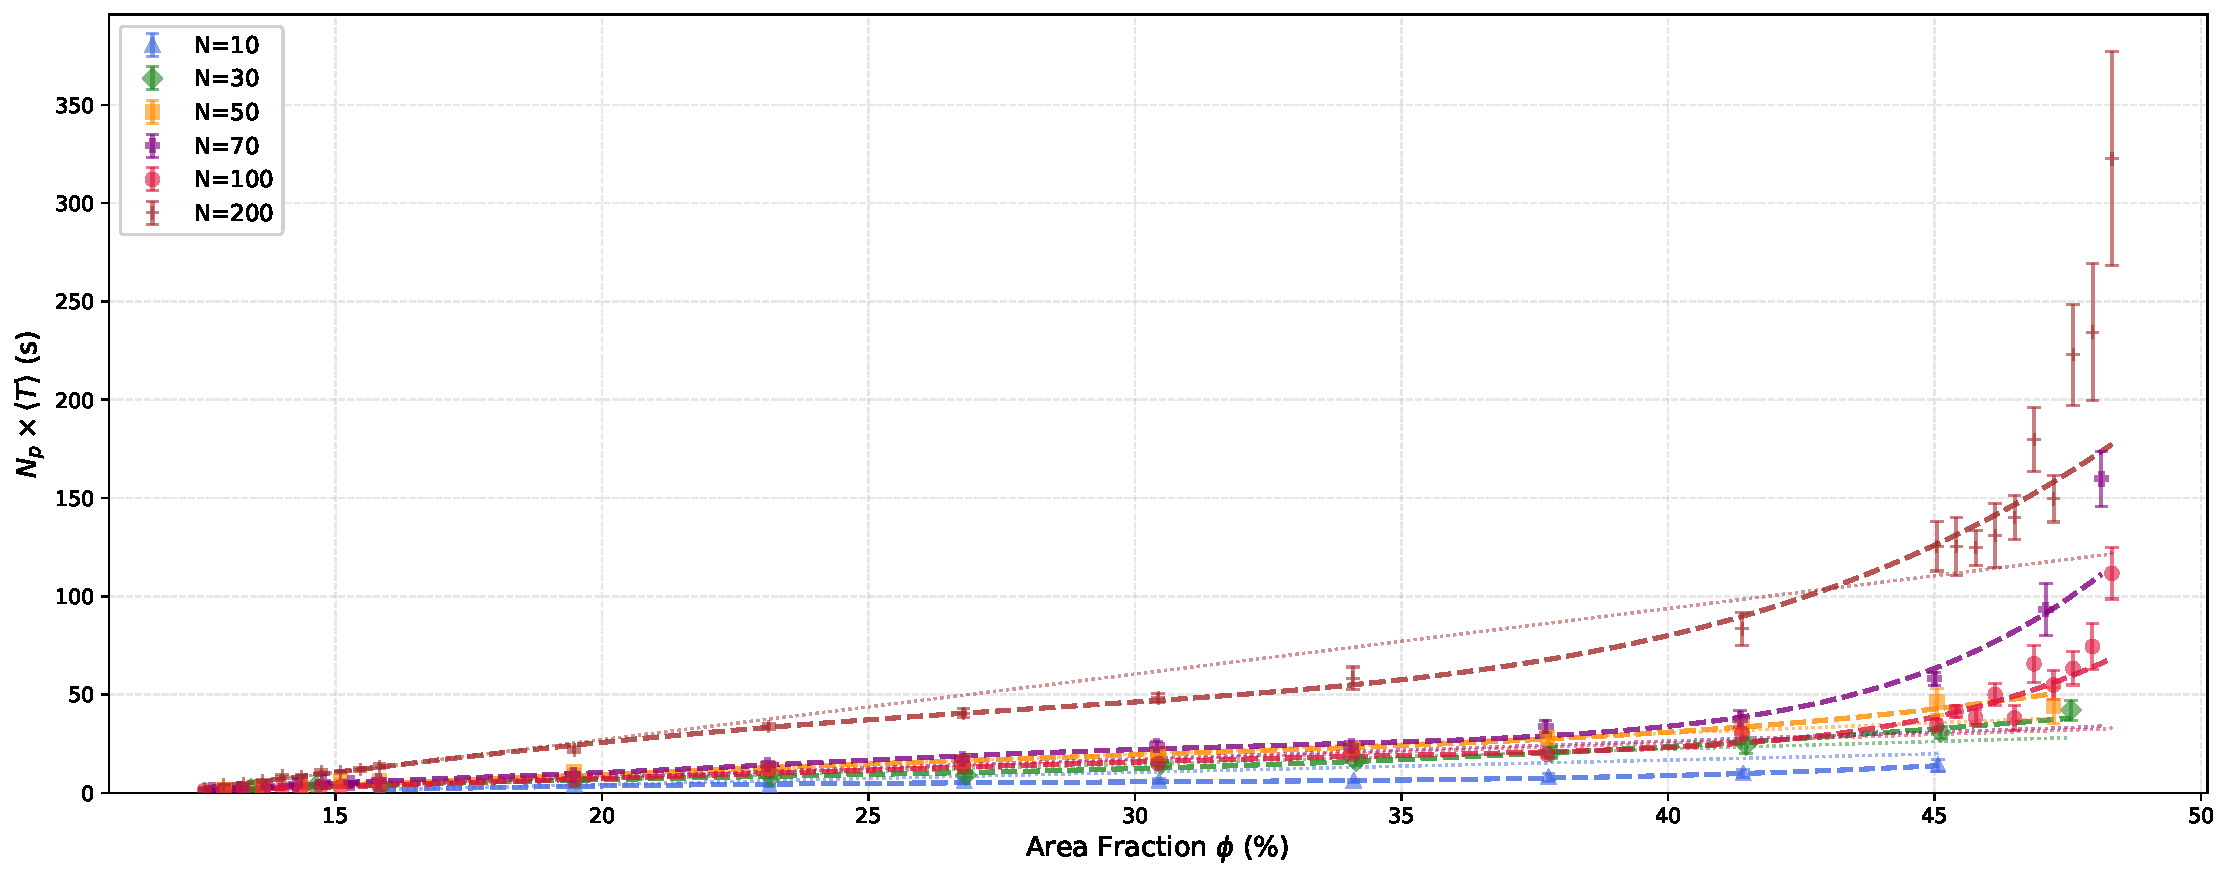
\includegraphics[width = 0.95\linewidth]{figures/FigB_ergodic_overlay.pdf}
    \caption{Overlay of the ergodic product $E = N_p \times \langle T \rangle$ versus area fraction $\phi$ for all six system sizes, illustrating that the departure from ideal, ergodic $1/N_p$ scaling occurs at a similar $\phi$ across systems despite the very different absolute magnitudes of $E$.}
    \label{fig:OverlayErgodicProduct}
\end{figure}

\textbf{Figure~\ref{fig:OverlayErgodicProduct}} shows the six ergodic-product curves placed on a common $\phi$ axis
spanning more than an order of magnitude in absolute scale, from roughly 20\,s at $N_\text{total} = 10$ to over 300\,s at $N_\text{total} =200$, yet all six begin bending away from linear growth in roughly the same window of area fraction, visually clustered between about $\phi\approx 30\%$ and $45\%$. The larger systems ($N_\text{total} = 70, 100, 200$) show the clearest, most steeply rising departures in this view, consistent with their sharper individual plots above, while the $N_\text{total} = 10$ and 30 curves remain closer to their respective extrapolations across most of the shared axis, only diverging visibly at the highest sampled $\phi$.

The clarity of the sub-critical-extrapolation departure differs markedly by system size. In the $N_\text{total} =10$ and 30 systems, the departure is gradual and its error bars are wide enough relative to the signal that an unambiguous departure point is difficult to identify. In the $N_\text{total} =70$, 100, and 200 systems, by contrast, the departure is sharp and resolvable well within the error bars, and, importantly, it becomes visible at a lower $N_p$ than the corresponding upward inflection in the raw $\langle T \rangle$ curve of Section~\ref{sec:4.2}. For the $N_\text{total} =100$ system, $E$ departs visibly from its extrapolation by rought $N_p \approx 70$--80, while the equivalent upturn does not become visually unambiguous in $\langle T\rangle$ itself (Figure~\ref{fig:Caldera100}) until closer to $N_p \approx 90$ which gives ergodic product a lead of some twenty to thirty probes. A comparable lead is visible for $N_\text{total}=200$ (departure near $N_p \approx 150$--165 in Figure~\ref{fig:ErgodicProduct200}, versus a visible $\langle T \rangle$ upturn closer to $N_p \approx 180$ in Figure~\ref{fig:Caldera200}).

\section{Detection Time Distributions: The Violin Plots}
\label{sec:4.5}

\begin{figure}[htbp]
    \centering
    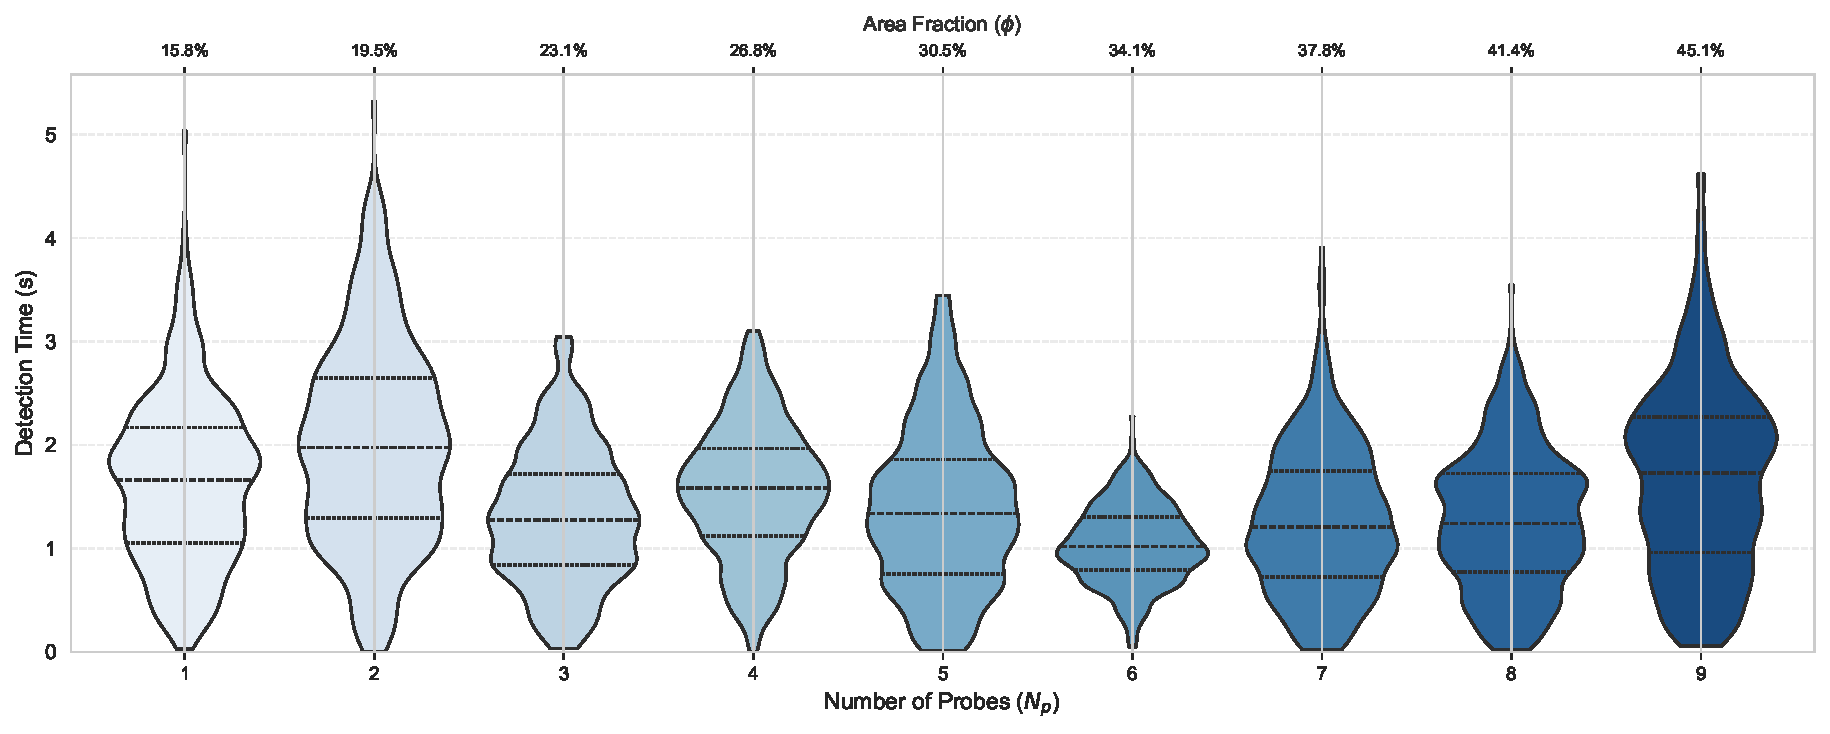
\includegraphics[width = 0.95\linewidth]{figures/violin_individual_N_10.pdf}
    \caption{Violin plots of the first-passage detection-time distribution as a function of probe number $N_p$ (bottom axis) and area fraction $\phi$ (top axis) for the $N_\text{total} = 10$ system, with each violin generated from a Gaussian approximation matched to that condition's ensemble mean and standard deviation (Section~\ref{sec:3.11}).}
    \label{fig:Violin10}
\end{figure}

\textbf{Figure~\ref{fig:Violin10}} ($N_\text{total} = 10$) shows nine violins who are all comparatively wide relative to their medians, consistent with this system's small ensemble and coarse $N_p$ sampling noted in Section~\ref{sec:4.1}. The narrowest violin occurs near $N_p = 6$, matching the fitted optimum in Table~\ref{tab:caldera-optima}, but the difference in width between this violin and its neighbors is modest where the widest and most visibly asymmetric violin appears at the crowded end, $N_p =9$, where the upper tail extends well past 4\,s.


\begin{figure}[htbp]
    \centering
    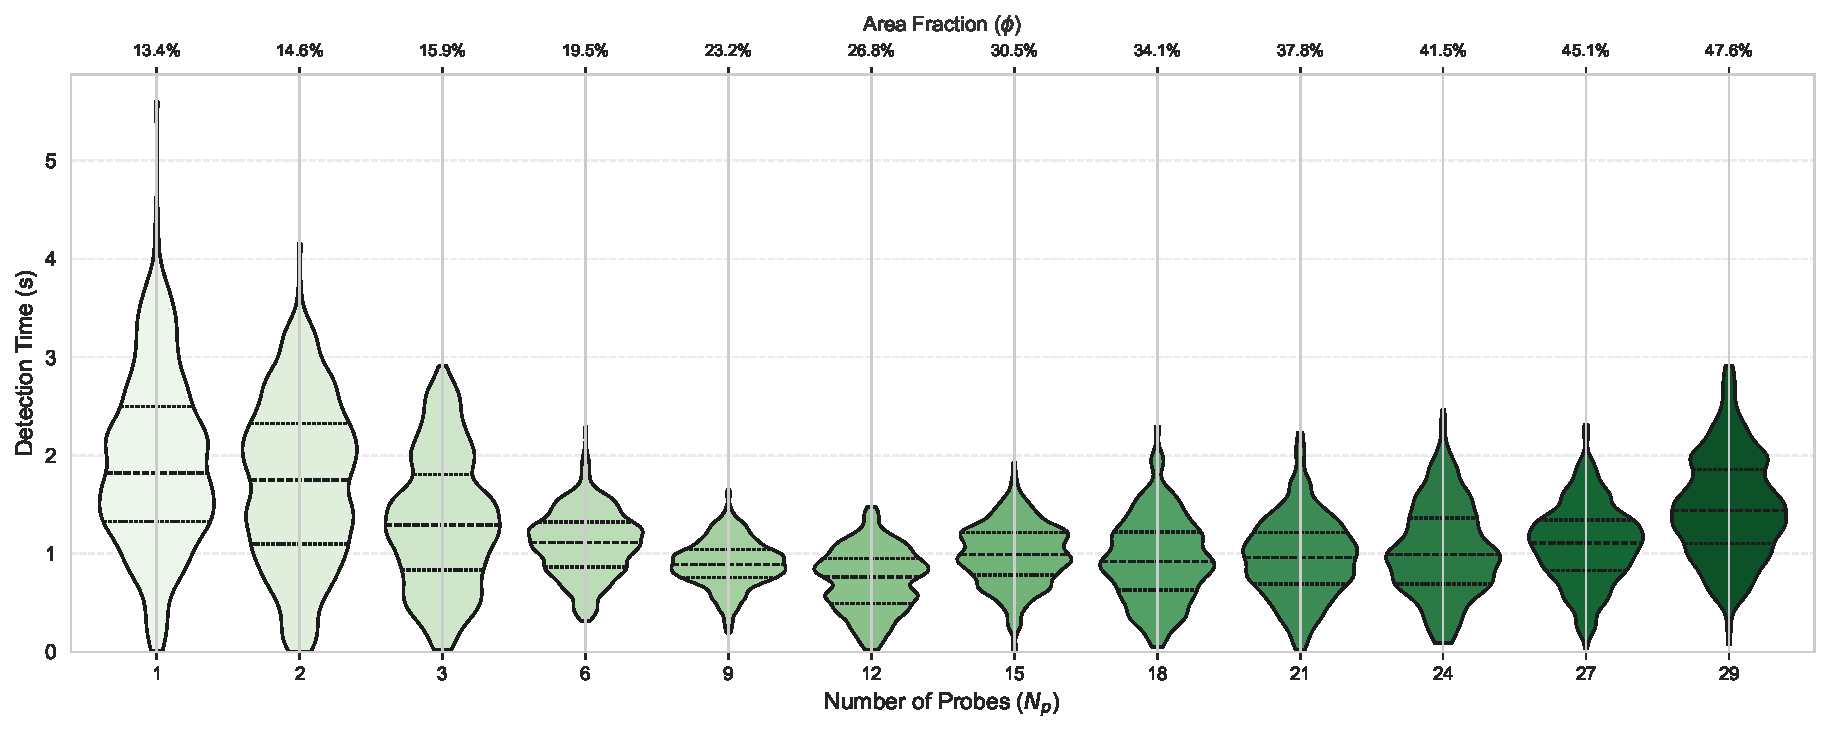
\includegraphics[width = 0.95\linewidth]{figures/violin_individual_N_30.pdf}
    \caption{Violin plots of the first-passage detection-time distribution as a function of probe number $N_p$ (bottom axis) and area fraction $\phi$ (top axis) for the $N_\text{total} = 30$ system, with each violin generated from a Gaussian approximation matched to that condition's ensemble mean and standard deviation (Section~\ref{sec:3.11}).}
    \label{fig:Violin30}
\end{figure}

\textbf{Figure~\ref{fig:Violin30}} ($N_\text{total} = 30$) shows a progression from wide to narrow to wide again that is clearer here than at $N_\text{total} =10$. The $N_p =1$--2 violins are tall and diffuse, the distribution from roughly $N_p =9$ to $18$ are visibly the most compact of the set, and the violins broaden again gradually toward $N_p = 29$, though the final violin remains narrower and less skewed than the crowded-end violins of the larger systems described below.

\begin{figure}[htbp]
    \centering
    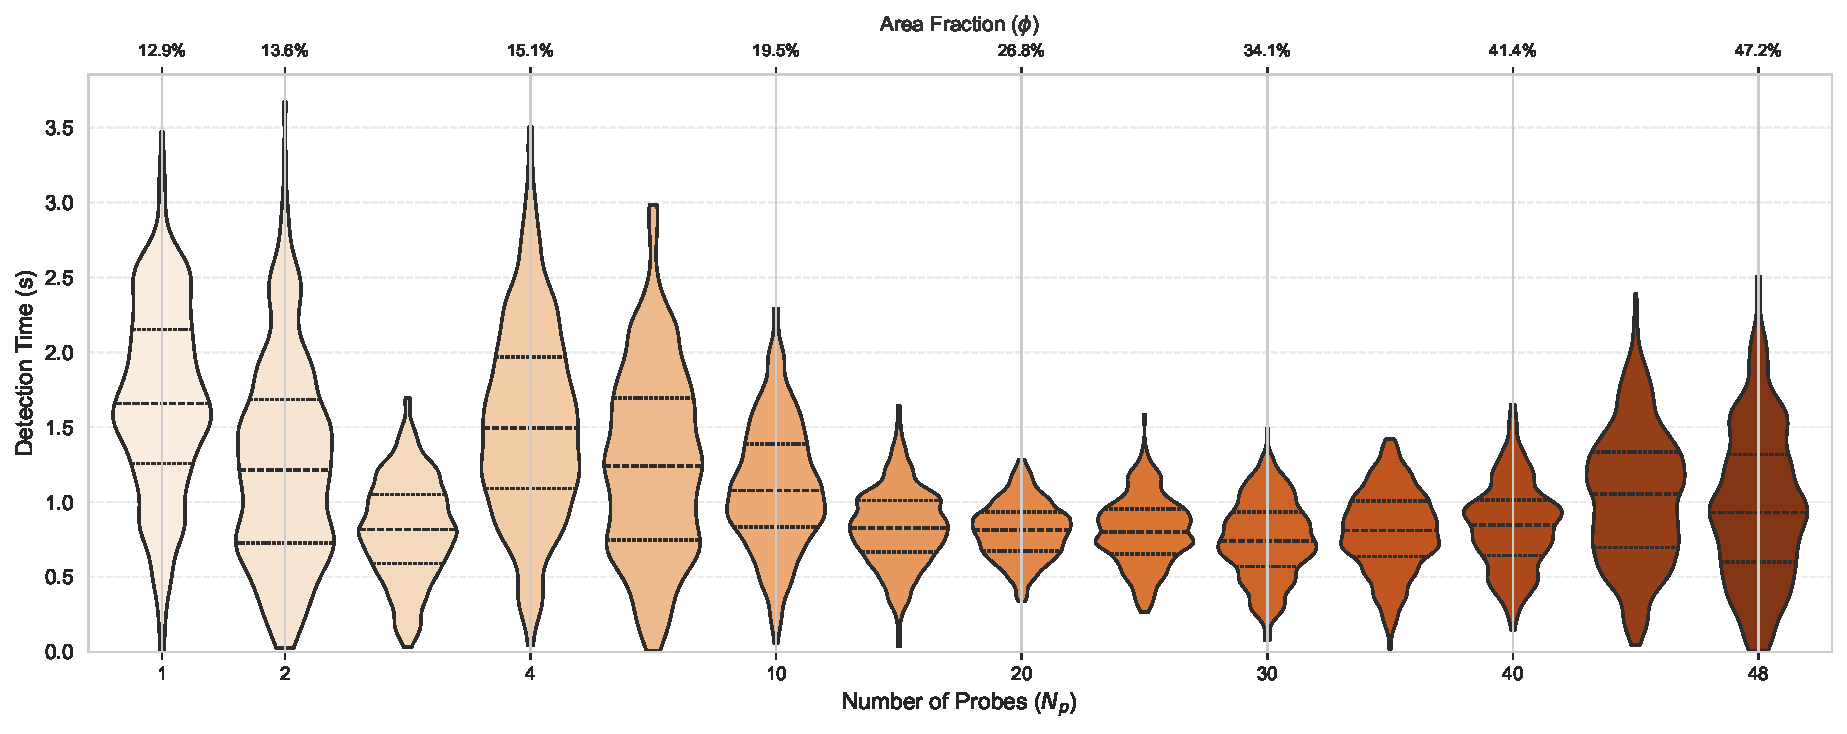
\includegraphics[width = 0.95\linewidth]{figures/violin_individual_N_50.pdf}
    \caption{Violin plots of the first-passage detection-time distribution as a function of probe number $N_p$ (bottom axis) and area fraction $\phi$ (top axis) for the $N_\text{total} = 50$ system, with each violin generated from a Gaussian approximation matched to that condition's ensemble mean and standard deviation (Section~\ref{sec:3.11}).}
    \label{fig:Violin50}
\end{figure}

\textbf{Figure~\ref{fig:Violin50}} ($N_\text{total} = 50$) shows that the violins at $N_p = 1$ and, especially, $N_p =4$ are the talles and most visibly right-skewed of the dilute-end conditions, echoing the early non-monotonicity seen in $\langle T \rangle$ for this system (Figure~\ref{fig:Caldera50}). The distributions tighten substantially from roughly $N_p =10$ through $30$, forming the flattest, most symmetric stretch the violins in the plot, before widening again at $N_p = 40$ and 48, where the upper tails begin to extend visibly beyond 2\,s.

\begin{figure}[htbp]
    \centering
    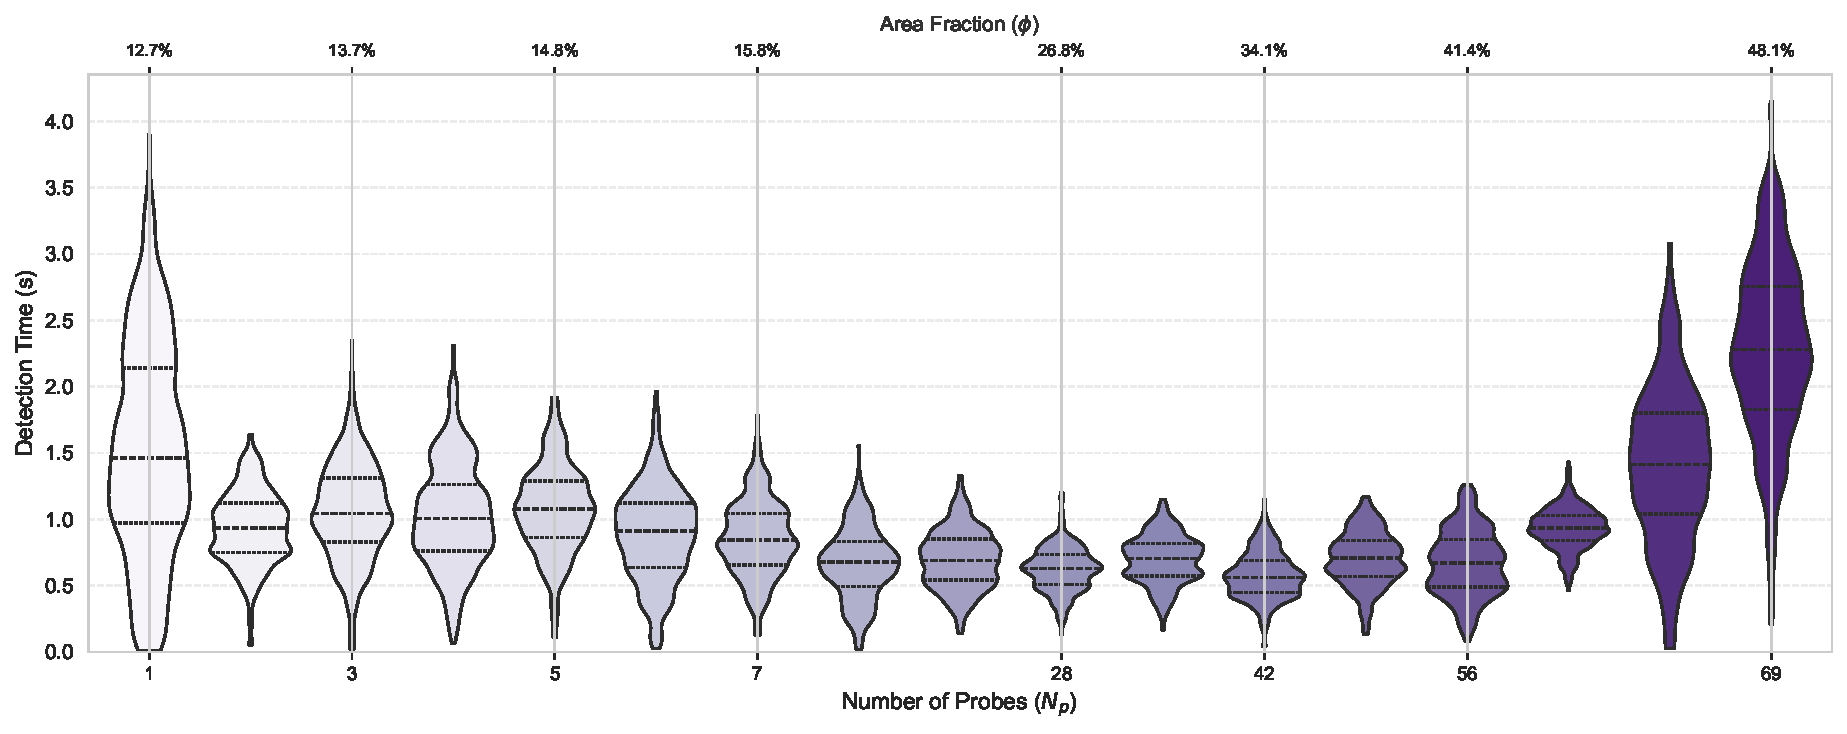
\includegraphics[width = 0.95\linewidth]{figures/violin_individual_N_70.pdf}
    \caption{Violin plots of the first-passage detection-time distribution as a function of probe number $N_p$ (bottom axis) and area fraction $\phi$ (top axis) for the $N_\text{total} = 70$ system, with each violin generated from a Gaussian approximation matched to that condition's ensemble mean and standard deviation (Section~\ref{sec:3.11}).}
    \label{fig:Violin70}
\end{figure}

\textbf{Figure~\ref{fig:Violin70}} ($N_\text{total} = 70$) shows violins with the contrast between the flat middle of the sweep and its crowded edge is the sharpest yet. The violin from roughly $N_p = 7$ through $58$ are visibly compact and close to symmetric, while the final two violins, at $N_p = 69$ and the point just before it, are both taller and more clearly right-skewed than any distribution earlier in the sweep, with upper tails reaching past 3\,s while the bulk of the density remains below 1.5\,s.

\begin{figure}[htbp]
    \centering
    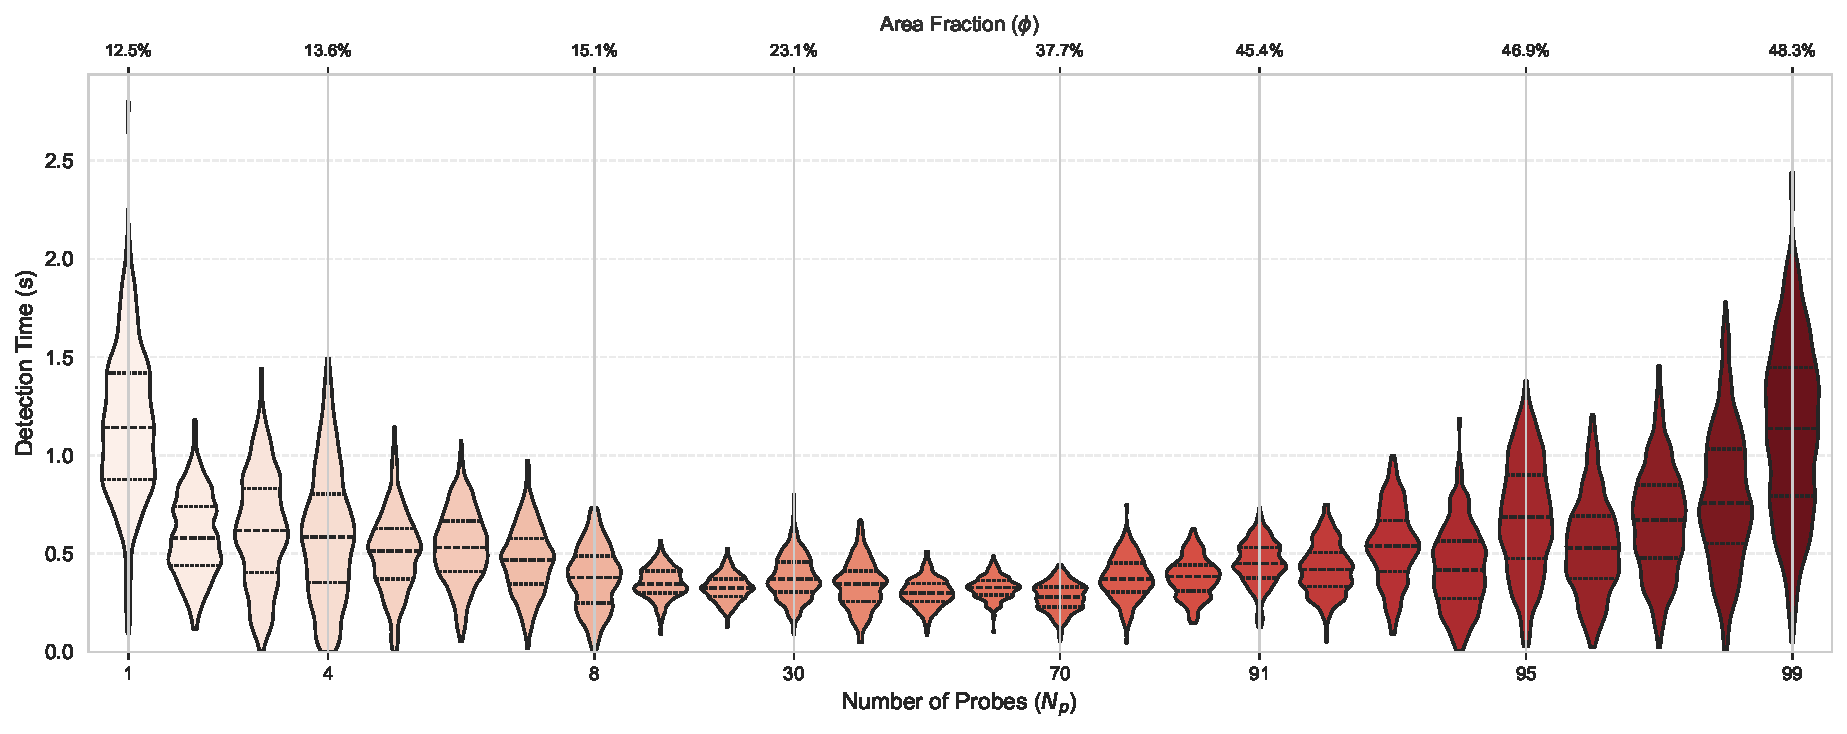
\includegraphics[width = 0.95\linewidth]{figures/violin_individual_N_100.pdf}
    \caption{Violin plots of the first-passage detection-time distribution as a function of probe number $N_p$ (bottom axis) and area fraction $\phi$ (top axis) for the $N_\text{total} = 100$ system, with each violin generated from a Gaussian approximation matched to that condition's ensemble mean and standard deviation (Section~\ref{sec:3.11}).}
    \label{fig:Violin100}
\end{figure}

\textbf{Figure~\ref{fig:Violin100}} ($N_\text{total} = 100$) shows twenty violins plotted and the clearest gradual narrowing and re-widening of the six systems. The violin width decreases steadily from $N_p =1$ to a visibly flat, thin band spanning roughly $N_p 3=0$ to $70$, then re-expands progressively toward $N_p = 99$. The last three or four violins are also the most visibly right-skewed of the set up to this point in the sweep, with medians that shift upward alongside the widening tails which is a shape echoed even more strongly in the $N_\text{total} =200$ system below.

\begin{figure}[htbp]
    \centering
    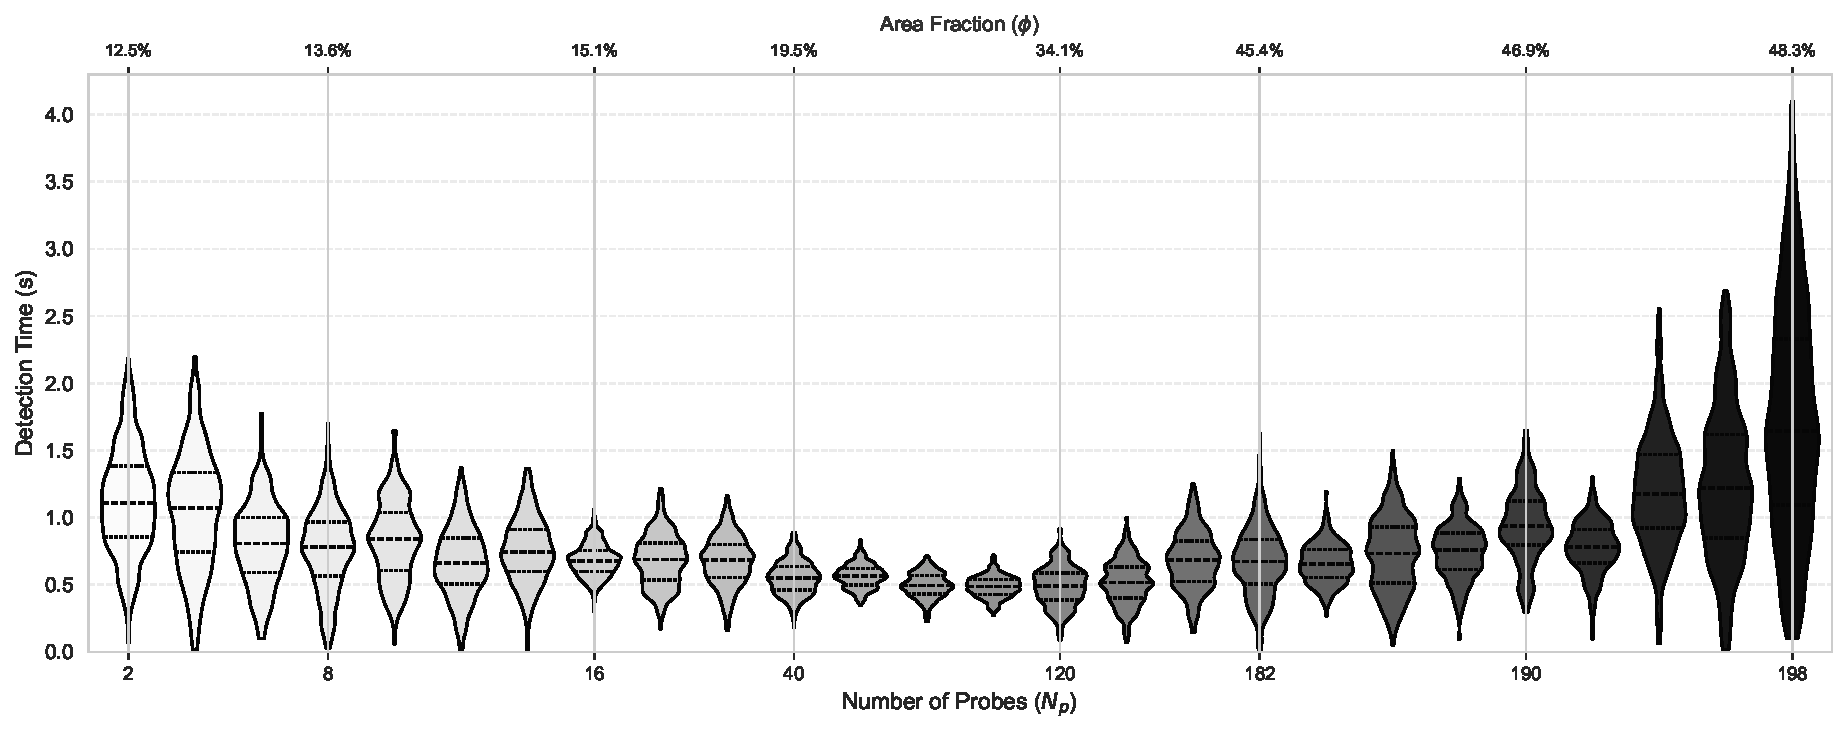
\includegraphics[width = 0.95\linewidth]{figures/violin_individual_N_200.pdf}
    \caption{Violin plots of the first-passage detection-time distribution as a function of probe number $N_p$ (bottom axis) and area fraction $\phi$ (top axis) for the $N_\text{total} = 200$ system, with each violin generated from a Gaussian approximation matched to that condition's ensemble mean and standard deviation (Section~\ref{sec:3.11}). Showing the most pronounced broadening and right-skewing of any system size at the most crowded conditions sampled.}
    \label{fig:Violin200}
\end{figure}

\textbf{Figure~\ref{fig:Violin200}} ($N_\text{total} = 200$) shows the most dramatic distributional change of the entire sweep. The violins across the broad middle of the range (roughly $N_p =40$ to $165$) are thin, symmetric, and nearly indistinguishable from one another in shape, but the final several violins, from around $N_p = 182$ onward, grow markedly taller and visibly right-skewed, with the $N_p = 198$ violin extending past 4\,s while its median remains well below that value showing the clearest visual signature in this thesis of a small number of runs taking substantially longer to detect than the typical run at the same condition.

\begin{figure}[htbp]
    \centering
    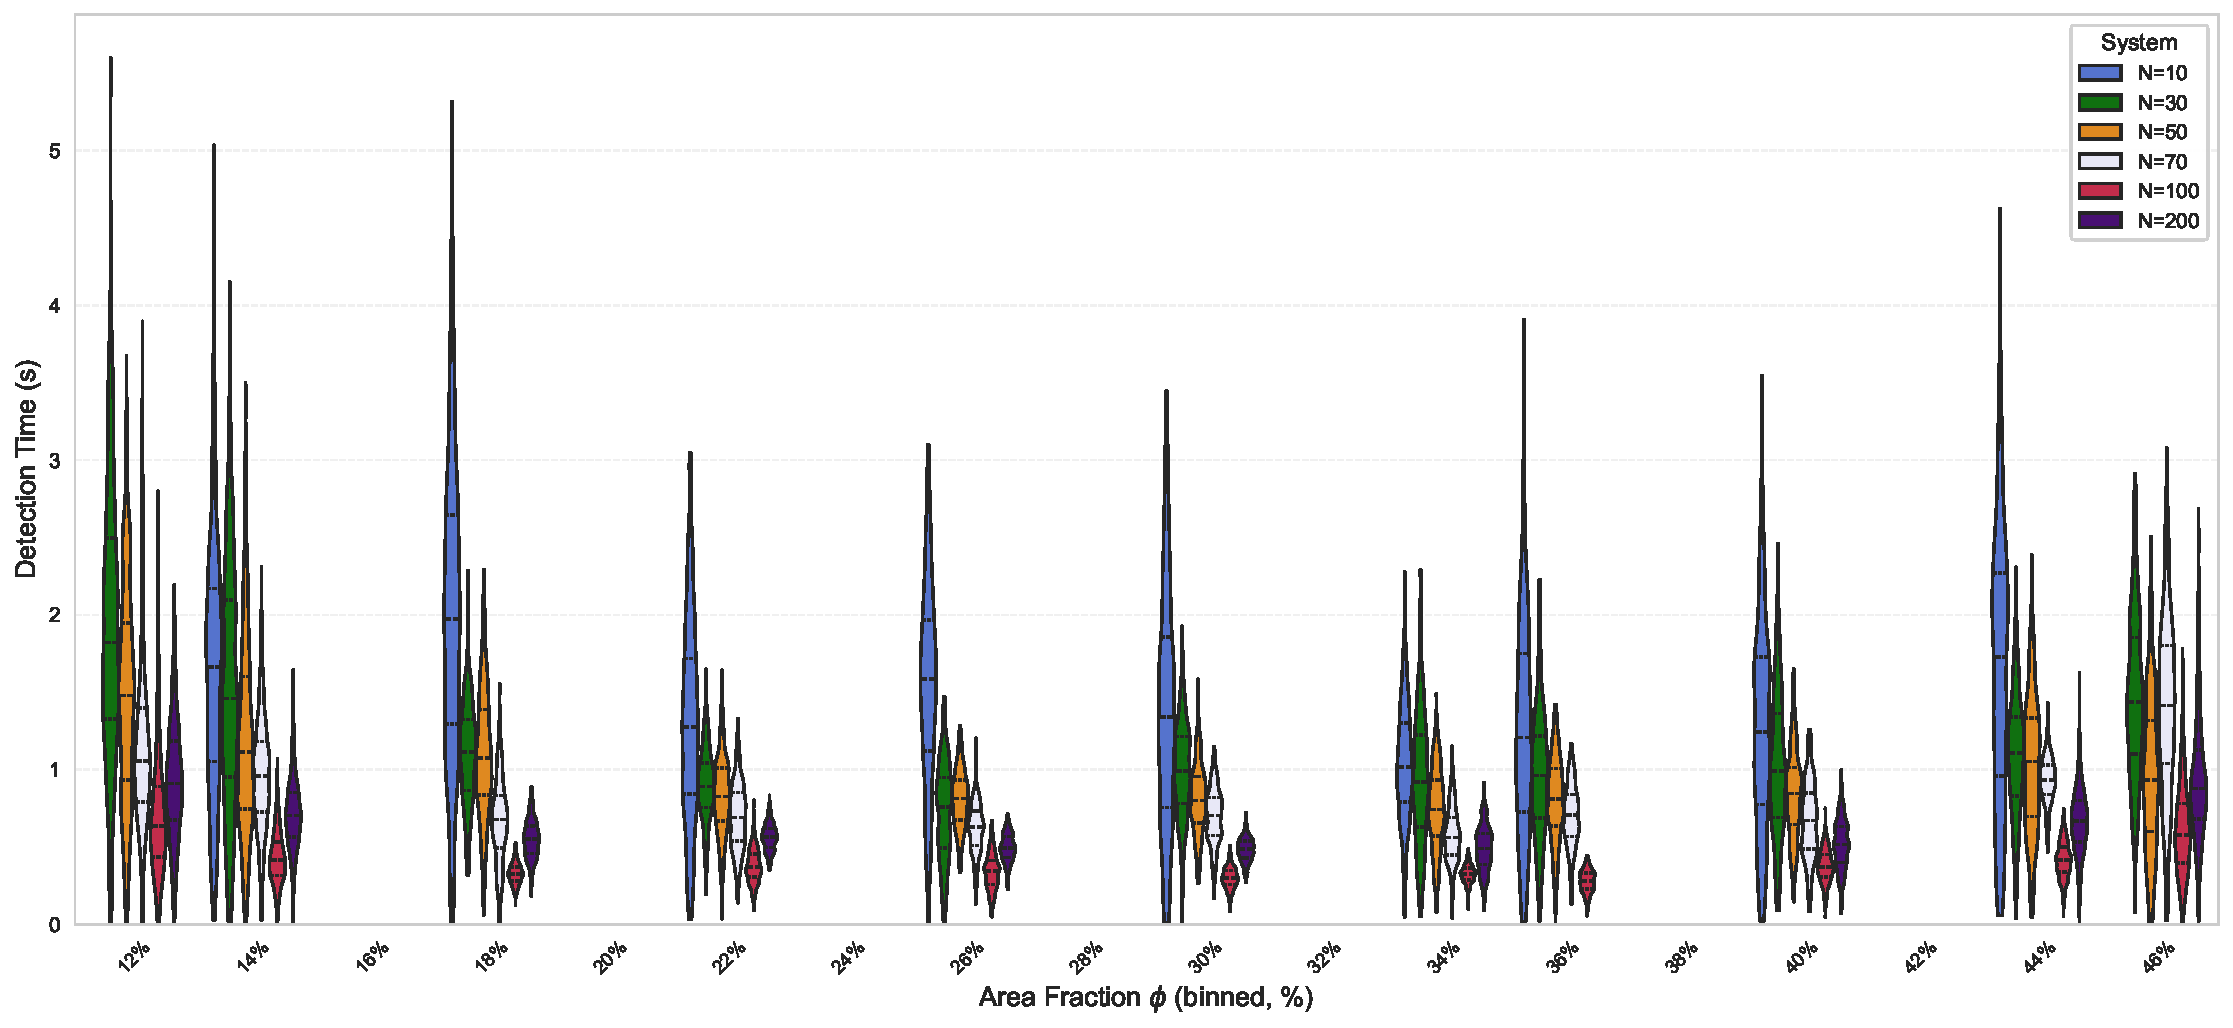
\includegraphics[width = 0.95\linewidth]{figures/FigD_violin_overlay.pdf}
    \caption{Composite violin plot comparing the detection-time distribution across all six system sizes, binned by area fractions $\phi$, with each system color-coded. This view shows how both the central tendency and the shape of the distribution evolve with crowding consistently across system scales.}
    \label{fig:OverlayViolin}
\end{figure}

\textbf{Figure~\ref{fig:OverlayViolin}} bins all six systems onto a common $\phi$ axis showing that, despite their very different absolute $N_p$ ranges, the six color-coded families of violins narrow toward their individually tightest shapes in roughly the same middle bins of the shared axis (broadly $\phi \approx 20$--35\%) and widen again together in the bins beyond about $\phi \approx 40\%$. The $N_\text{total} = 10$ family (narrowest range of bins populated, owing to its coarse sampling) and the $N_\text{total} = 200$ family (populating the most bins, and showing the tallest, most skewed violins at the crowded end) sit at opposite extremes of this composite view, with the four intermediate system sizes arranged between them in a consistent, overlapping progression.

Taken together, the violin plots (Figures~\ref{fig:Violin10}--\ref{fig:OverlayViolin}) show a consistent evolution in distribution shape across the prove-density sweep, in every system. Broad and occasionally asymmetric distribution at the dilute end ($N_p = 1$--2), narrowing to their tightest and most symmetric near the caldera floor, and broadening  again, with visible right-skew, toward the crowded end of the sweep. The severity of this crowded-end broadening differs by system size. The $N_\text{total} = 200$ system shows the most pronounced broadening and right-skewing of any system at its most crowded sampled conditions, while the $N_\text{total} =10$ system shows comparatively modest change in shape between its floor and crowded-end violins. The composite plot binned by area fraction shows that this evolution in shape occurs at a similar $\phi$ across system sizes, reinforcing $\phi$, rather than raw $N_p$ or $N_\text{total}$, as the more natural variable for comparing search behavior across scales.

\section{Typology for the Caldera profiles}
\label{sec:4.6}

Four types of "caldera" inspired by volcanology.

\textbf{Type I - Incipient (Latent) Caldera.} A minimum exists in the fit, but the apparent rise on the crowded side is comparable to or smaller than the run-to-run standard error, so the crowding side cannot be distinguished from statistical noise given ten seeds and the coarse, low-Np integer sampling available at small $N_\text{total}$. What's included here is $N_\text{total} = 10$.

\textbf{Type II - Shield Caldera.} The minimum is statistically resolvable and a genuine, monotonic rise appears at high $N_p$, but the rise is modest. a broad, gently sloping floor rather than a sharp wall, with the crowded-side $\langle T \rangle$ reaching only roughly 1.1-1.8$\times$ the floor value. What's included here are $N_\text{total} = 30$ and 50.

\textbf{Type III - Steep-Walled (Stratovolcano) Caldera.} A long, flat, low-variance diffusion limited plateau in a sharp, unambiguous upturn near the top of the sampled Np range, with $\langle T \rangle$ rising to roughly 2-5$\times$ the floor value and the standard deviation widening in step. The ergodic product for these systems also breaks from its sub-critical extrapolation well before the rise is visible in $\langle T \rangle$ alone. Examples of this type of caldera includes $N_\text{total} = 70$, 100, 200.

\textbf{Type IV - Bifurcated (Double-floor) Caldera}. A small number of systems display a caldera floor that does not settle into a single, uninterrupted minimum. Instead, the $\langle T \rangle$ versus $N_p$ profile dips to a first low point, rises gently, and dips again to a second low point before finally climbing into the crowding-limited regime on the far side. Visually, this resembles a caldera with two adjacent low points along its floor rather than one continuous basin. The clearest of this pattern appears in the $N = 100$ system, where a shallow first floor near $N_p\approx 15$--20 is followed by a modest rise and then a deeper second floor near $N_p \approx 50$--70. A weaker, less pronounced version of the same shape is also visible in the $N=70$ profile. We introduce Type IV here as a qualitative addition to the caldera typology, identified descriptively by its floor shape in the same manner as Types I, II, and III.

This typology is not confined to the caldera fit alone, it is corroborated by the other two diagnostics. The Type I system ($N_\text{total} = 10$) show sthe least resolvable departure in the ergodic product (Section~\ref{sec:4.4}) and the least dramatic change in violin shape (Section~\ref{sec:4.5}) between its floor and crowded conditions. The Type II systems ($N_\text{total} = 30$, 50) show a modest but genuine departure in both. The Type III systems ($N_\text{total} = 70$, 100, 200) show sharp, well-resolved signatures across all three diagnostics simultaneously --- the caldera fit, the ergodic product, and the violin plot broadening all sharpen together as system size grows.

\section{The Agreement of the Three Diagnostics}
\label{sec:4.7}

Three methodologically independent diagnostics, being the parametric caldera fit's minimum (Section~\ref{sec:4.2}), the ergodic product's departure from ideal linear scaling (Section~\ref{sec:4.4}), and the qualitative broadening of the detection-time distribution (Section~\ref{sec:4.5}), converges on locating the crowding transition within a similar area-fraction band, roughly $\phi \approx 28$--35\%, across all six system sizes. This convergence matters because the three diagnostics make different assumptions. The caldera fit assumes a specific two-term functional form (Equation~\ref{eq:3.6}), the ergodic product assumes only that ideal search behaves as a flat line in $N_p$, and the violin-plot broadening assumes nothing beyond the shape of the sampled distribution itself. That three routes with little in common beyond the underlying data arrive at the same transition window makes it unlikely that $\phi^* \approx 30\%$ is an artifact of any single analytical choice, such as the exponents or amplitude bounds used in the nonlinear least-squares fit. The agreement is tightest for the Type III systems ($N_\text{total} = 70,100,200$), where all three diagnostics are individually well-resolved and mutually consistent. The agreement is loosest for the Type I and Type II systems ($N_\text{total}= 10, 30, 50$), where each diagnostic is individually less statistically confident, a limitation attributable to the small number of discrete $N_p$ values available at low $N_\text{total}$ (Section~\ref{sec:3.1}) rather than to any disagreement in the underlying physics.

\section{Sensitivity Hypothesis Confirmation}
\label{sec:4.8}
Section~\ref{sec:1.3} posed the ergodic product as a candidate for detecting the onset of crowding earlier than $\langle T \rangle$ alone. The results in Section~\ref{sec:4.4} confirm this, at least for the Type III systems where $E$ departs from its ideal linear extrapolation some twenty to thirty probes before the corresponding rise is visually unambiguous in the raw $\langle T \rangle$ curve. A plausible mechanistic reason is that $E = N_p \times \langle T \rangle$ converts a small multiplicative deviation from ideal $1/N_p$ scaling directly into a deviation from a flat baseline, whereas the same deviation, expressed in $\langle T \rangle$ itself, is masked by the still-declining $1/N_p$ trend until the deviation grows large enough to visibly overcome that decline. In effect, $E$ re-expresses a subtle relative slowdown as an absolute, additive departure from a constant, which is easier to distinguish from measurement noise than the same slowdown buried in an already-falling curve. This sensitivity advantage is clearest for the systems with the most $N_p$ sampling points and the tightest error bars ($N_\text{total} = 70,100,200$). As for $N_\text{total} = 10$ and 30, the hypothesis is not denied, but the advantage cannot be established with confidence given the available sampling density which is an important caveat for any point-of-care application operating at low absolute particle counts, where the extra sensitivity this thesis reports may not be practically realizable.

\section{A complication for Ideal Search Theory}
\label{sec:4.9}
The ideal $1/N_p$ scaling law (Section~\ref{sec:2.3}) is a dilute-limit statement, and classical intuition about when that limit breaks down often defaults to geometric packing constraints which is also the assumption that searchers only meaningfully interfere with one another as the system approaches close packing. The results here complicate that intuition considerably. Across all six systems, the crowding-limited regime sets in within a band corroborated by all three diagnostic of Section~\ref{sec:4.7}, $\phi \approx28$--35\%, and most precisely located within that band by the parametric caldera fit at $\phi^* \approx 29$--31\% (Table~\label{ref:4.1}), roughly one-third of the hexagonal close-packing ceiling ($\phi_\text{HCP} \approx 90.7\%$, Section~\ref{sec:1.2}) and well under the highest area fraction actually sampled in this study ($\approx 48\%$). This indicates that the breakdown documented here is a dynamical phenomenon, driven by caging and mutual interference among diffusing, finite-sized probes during active search, rather than a simple consequence of running out of physical space. Practically, this means that treating a system as ``dilute enough'' because it is geometrically far from close packing is not a safe assumption --- area fractions that would still be called sparse by a packing-fraction standard (40--50\%, for instance) are already well past the point where this study finds the ideal, non-interacting search law to have broken down.

\section{An Open Question: The Non-Monotonic Role of System Size}
\label{sec:4.10}
While $\phi^*$ is strikingly stable across system size (Sections~\ref{sec:4.2}), \ref{sec:4.7}, the absolute floor value of $\langle T \rangle$ is not monotonic in $N_\text{total}$. It falls from roughly 1.0\,s ($N_\text{total} = 10$) to roughly 0.3\,s ($N_\text{total} = 100$), which is the expected direction since a larger system has proportionally more foreign targets at the same $\phi$, so a probe should on average need less time to encounter one. But the floor then rises again at roughly 0.5\,s at $N_\text{total} = 200$, reversing that trend, a reversal already visible directly in Figure~\ref{fig:OverlayCaldera}. Several explanations are possible, and none is conclusively ruled out by the present data as this could reflect a genuine finite-size crossover in how caging onset interacts with the growing absolute number of foreign targets; it could be an artifact of the fixed 10-seed ensemble becoming a less adequate sample as the box grows and detection events become rarer per unit area; or it could reflect a subtlety in how box side length $L$ and periodic boundary geometry interact with the fixed 2:1 probe-to-foreign diameter ratio as $L$ grows. Distinguishing between these possibilities would require additional system sizes bracketing $N_\text{total} = 100$--200 and beyond 200, which is beyond the present scope but is flagged here as a direct extension of this work.

\section{Detection Fraction at the Crowded Edge}
\label{sec:4.11}
Section~\ref{sec:3.8} noted that any simulation run failing to reach $R_\text{int}$ within the 2.0\,s production window is excluded from that condition's mean, so the reported $\langle T \rangle$ at the most crowded, slowest-detecting $N_p$ values is conditioned only on the seeds that succeeded which is a lower-bound estimate rather than a true mean over all attempts. This caveat is most relevant precisely where it is least convenient in which the sharp, Type III crowded-side upturns ($N_\text{total}=70,100,200$; Figures~\ref{fig:Caldera70}--\ref{fig:Caldera200}) are exactly the conditions most likely to have a reduced detection fraction, since these are the slowest-detecting, most heavily caged conditions in the entire sweep. If the detection fraction falls meaningfully below 1.0 at these points, the true crowding penalty is understated by the figures presented in this chapter wherein the caldera's crowded-side wall may in fact be steeper than reported. Per-condition detection fraction were tracked during extraction (Section~\ref{sec:3.11}) but have not yet been reported as a figure in this chapter; doing so, by flagging any condition below the 0.9 threshold used during extraction, would allow a reader to judge exactly how conservative the reported upturns are, and is recommended as an addition before this chapter is finalized.
% The sentence from "per-condition detection fraction were..." needs to be checked here, I am not sure if it is correct, especially after checking Section 3.5 mentioned in this sequence

\section{Summary of Key Findings}
\label{sec:4.12}
Across six system sizes spanning $N_\text{total} =10$ to 200, mean first-passage detection time follows a consistent caldera shape in probe number: falling under diffusion-limited search at low $N_p$, reaching a minimum, and rising again under crowding-limited search at high $N_p$ (Section~\ref{sec:4.1}). The optimal probe density, located independently by a parametric caldera fit, sits at an area fraction of $\phi^* \approx 29$--31\% for five of the six systems studied, well below the geometric close-packing ceiling, indicating that the transition is dynamically rather than geometrically determined (Section~\ref{sec:4.2}, \ref{sec:4.9}). The ergodic product $E = N_p \times \langle T \rangle$ confirms the sensitivity hypothesis of Section~1.3 for the larger, Type III systems, flagging the onset of crowding tens of probes before the same transition becomes visible in $\langle T \rangle$ alone (Sections~\ref{sec:4.4}, \ref{sec:4.8}). Three independent diagnostics being the caldera fit, the ergodic product and the shape of the detection-time distribution converge on the same transition window, and a fourfold typology (Incipient, Shield, Steep-Walled, bifurcated) captures how the sharpness of this convergence itself scales with system size (Section~\ref{sec:4.6}, \ref{sec:4.7}). In addition to the three principal caldera shapes, the fourth, qualitatively distinct floor shape was observed in the $N=100$ system, and more faintly in $N=70$: rather than a single continuous minimum, the $\langle T \rangle$ versus $N_p$ curve traces two adjacent low points separated by a modest intervening rise. This pattern, termed a Bifurcated (Type IV) caldera, was not observed in the remaining systems studied, each of which retained the conventional single-floor profile. Two open items remain: a non-monotonic dependence of the absolute floor detection time on $N_\text{total}$ (Section~\ref{sec:4.10}), and an unreported detection-fraction diagnostic that may mean the crowded-side upturn documented here are conservative (Section~\ref{sec:4.11}). %%could be results and discussions
% !TEX root =  main.tex
\chapter{Summary and Conclusions}
\label{chap:5}
This thesis set out to answer a specific question left open by first-passage search theory: in a crowded, two-dimensional Brownian mixture, at what probe density does adding more searchers stop helping and start hindering detection, and can this transition be flagged earlier than by watching the mean detection time alone? Using Langevin dynamics simulations in LAMMPS, across six system sizes and a probe-density sweep from a single searcher to near-total population, this thesis confirms that a caldera-shaped trade-off exists, is not an artifact of any one system scale, and is quantifiable by more than one independent diagnostic.

The central results is that the optimal probe density, $\phi^*$, is consistent at roughly 29--31\% of the two-dimensional domain area across system sizes spanning a full order of magnitude ($N_\text{total} =30$ to 200), with a modestly elevated value at the smallest system studied ($N_\text{total}=10$). This optimum sits well below the theoretical hexagonal close-packing ceiling, which indicates that the breakdown of ideal, non-interacting search behavior is driven by dynamical caging effects during active search rather than by the searchers simply running out of physical room. The ergodic product, $E = N_p \times \langle T \rangle$, was confirmed as a more sensitive early indicator of this transition than the mean detection time alone, particularly for the larger, more heavily sampled system sizes, where it flagged the onset of crowding-influenced search tens of probes before the corresponding change became visually apparent in $\langle T \rangle$ itself. A threefold qualitative typology --- Incipient, Shield, and Steep-Walled caldera profiles --- was introduced to describe how the sharpness of this crowding response scales with the system size, and was shown to be corroborated independently by the ergodic product and the detection-time distribution shape, not solely by the parametric fit from which it was first drawn. In addition to the three primary caldera types, we observe a qualitatively distinct double-floor (bifurcated) shape in the $N=100$ system, with a weaker hint of the same pattern in $N=70$. We introduce this as a fourth caldera type, Type IV, and recommend it as a direction for future investigation with denser probe-number sampling.

% Beyond the three caldera types already identified, visual inspection of the $\langle T \rangle$ versus $N_p$ curves reveals a fourth, qualitatively distinct floor shape in the $N=100$ system where rather than a single continuous minimum, the curve traces two adjacent low points separated by a modest intervening rise. We classify this as a Bifurcated (Type IV) caldera. A similar, though considerably shallower, double dip shape is also visible in $N=70$, subtle enough that we regard it as a weaker instance of the same pattern rather than a clearly separate floor. The remaining systems each display conventional single-floor shape already captured by Types I-III.

These findings carry practical implications for point-of-care microfluidic and colloidal impurity-detection systems, where probe density is a design choice and not merely a fixed property of the sample. Rather than maximizing the number of functionalized probe particles introduced into a search volume, this work suggests that detection efficiency is optimized at a comparatively moderate, system-size-independent area fraction. Reducing not only detection time but also reagent cost and the risk of fluid clogging associated with overloading a sample with searchers. More broadly, by demonstrating a controlled, quantifiable breakdown of the ergodic $1/N_p$ scaling law well short of geometric packing limits, this work contributes a concrete data point to the wider study of non-equilibrium statistical mechanics in crowded, finite-sized environments which is a regime relevant to macromolecular crowding in biological cytoplasm as much as to synthetic colloidal suspensions.

This study has several limitations that bound the scope of these conclusions. The simulations are restricted to two dimensions, to purely repulsive Weeks-Chandler-Andersen interaction with no long-range electrostatics, hydrodynamics coupling, or gravitational effects, and to a fixed 2:1 probe-to-foreign diameter ratio. Each condition was averaged over ten independent seeds, and the production window was fixed 2.0\,s of simulated time, which may understate the true crowding penalty at the most heavily caged conditions if detection fractions there fall meaningfully below 1.0, as discussed in Section~\ref{sec:4.11}. The non-monotonic dependence of the absolute floor detection time on total system size (Section~\ref{sec:4.10}) also remains unresolved and is flagged as a direction for future work, alongside extending this framework to three dimensions, to a wider range of diameter ratios, and to explicit hydrodynamic interactions between probes.

Taken together, these results answer the question posed at the outset of this thesis: more searcher do not help without limit, and the point at which they stop helping is neither arbitrary  nor system-size-dependent in the way naive packing arguments would suggest. It is a stable, dynamically determined optimum, detectable earlier through the ergodic product than through raw detection time, and consistent enough across scales to serve as concrete, practical guidance for the design of crowded, particle-based detection systems.

%% you may add more chapters by including more files just as above.
%% see the files for patterns of the format used.

\appendix
% !TEX root =  main.tex
\chapter{Previous Published Results}

\section{SPP 2025 [1]: Lag Time in Diffusion Coefficient Estimation}
\label{appendix:pb30}

Section~\ref{sec:langevin-damping} introduced the Langevin damping parameter $\tau_{\text{damp}}$ and the requirement that the sampling time interval $\tau$ satisfy $\tau \gg \tau_{\text{damp}}$ before a measured diffusion coefficient can be trusted. This requirement, used throughout Chapter~3 to validate pure Brownian dynamics before any detection statistics were computed, was established in our earlier conference paper \cite{balejado2025}, which compared the mean-squared-displacement method ($D_{\text{MSD}}$) against the displacement-variance method ($D_{\text{var}}$) for polystyrene probes across a wide sweep of sampling intervals.

\begin{figure}[H]
    \centering
    \subfigure[Runtime duration: 1 million time steps\label{fig:3a}]{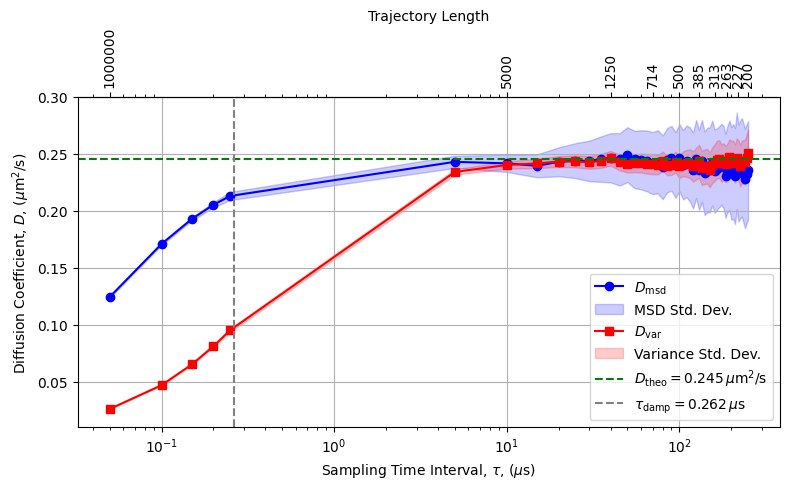
\includegraphics[width=0.45\textwidth]{figures/1mil.png}}
    \hspace{0.02\textwidth}
    \subfigure[Runtime duration: 5 million time steps\label{fig:3b}]{
    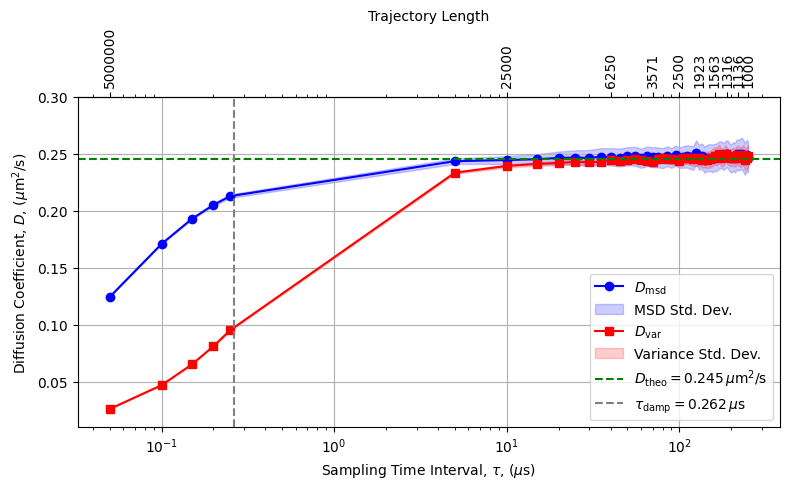
\includegraphics[width=0.45\textwidth]{figures/5mil.png}}
    \caption{$D_{\text{MSD}}$ and $D_{\text{var}}$ versus increasing sampling time interval $\tau$, from $25\,\mu\text{s}$ to $250\,\mu\text{s}$, for two total runtime durations. The green dashed line marks the theoretical Stokes-Einstein value $D_{\text{th}} = 0.245\,\mu\text{m}^2/\text{s}$; the gray dotted line marks $\tau_{\text{damp}} = 0.262\,\mu\text{s}$. Reproduced from \cite{balejado2025}.}
    \label{fig:appendix-pb30-fig3}
\end{figure}

Figure~\ref{fig:appendix-pb30-fig3} shows that both estimators underestimate $D$ when $\tau \le \tau_{\text{damp}}$, since the observed trajectory is still dominated by the ballistic, momentum-conserving regime rather than diffusive motion. Both methods converge toward $D_\text{th}$ once $\tau$ exceeds $\tau_\text{damp}$, with $D_\text{MSD}$ converging faster but $D_\text{var}$ retaining tighter precision at longer lag times, where the usable trajectory is shorter. This is the direct justification for the $\tau = 1.0\,\mu\text{s}$ sampling interval adopted throughout the present thesis (Section~\ref{sec:verifying-bm}), which sits safely inside the accurate-and-precise window identified here. 

\section{SPP 2026 [2]: Optimal Probe Density for Brownian First-Passage Detection}
\label{appendix:pa04}

Section~\ref{sec:study-gap} identified the open question this thesis answers in full. The question being whether a caldera-shaped minimum in $\langle T \rangle$ exists across probe density, and whether the ergodic product $E$ can flag the crowding transition earlier than $\langle T \rangle$ itself. That question was first posed, in preliminary form and for a single system size ($N_\text{total} = 100$), in our conference paper \cite{Balejado2026}.

\begin{figure}[b!]
    \centering
    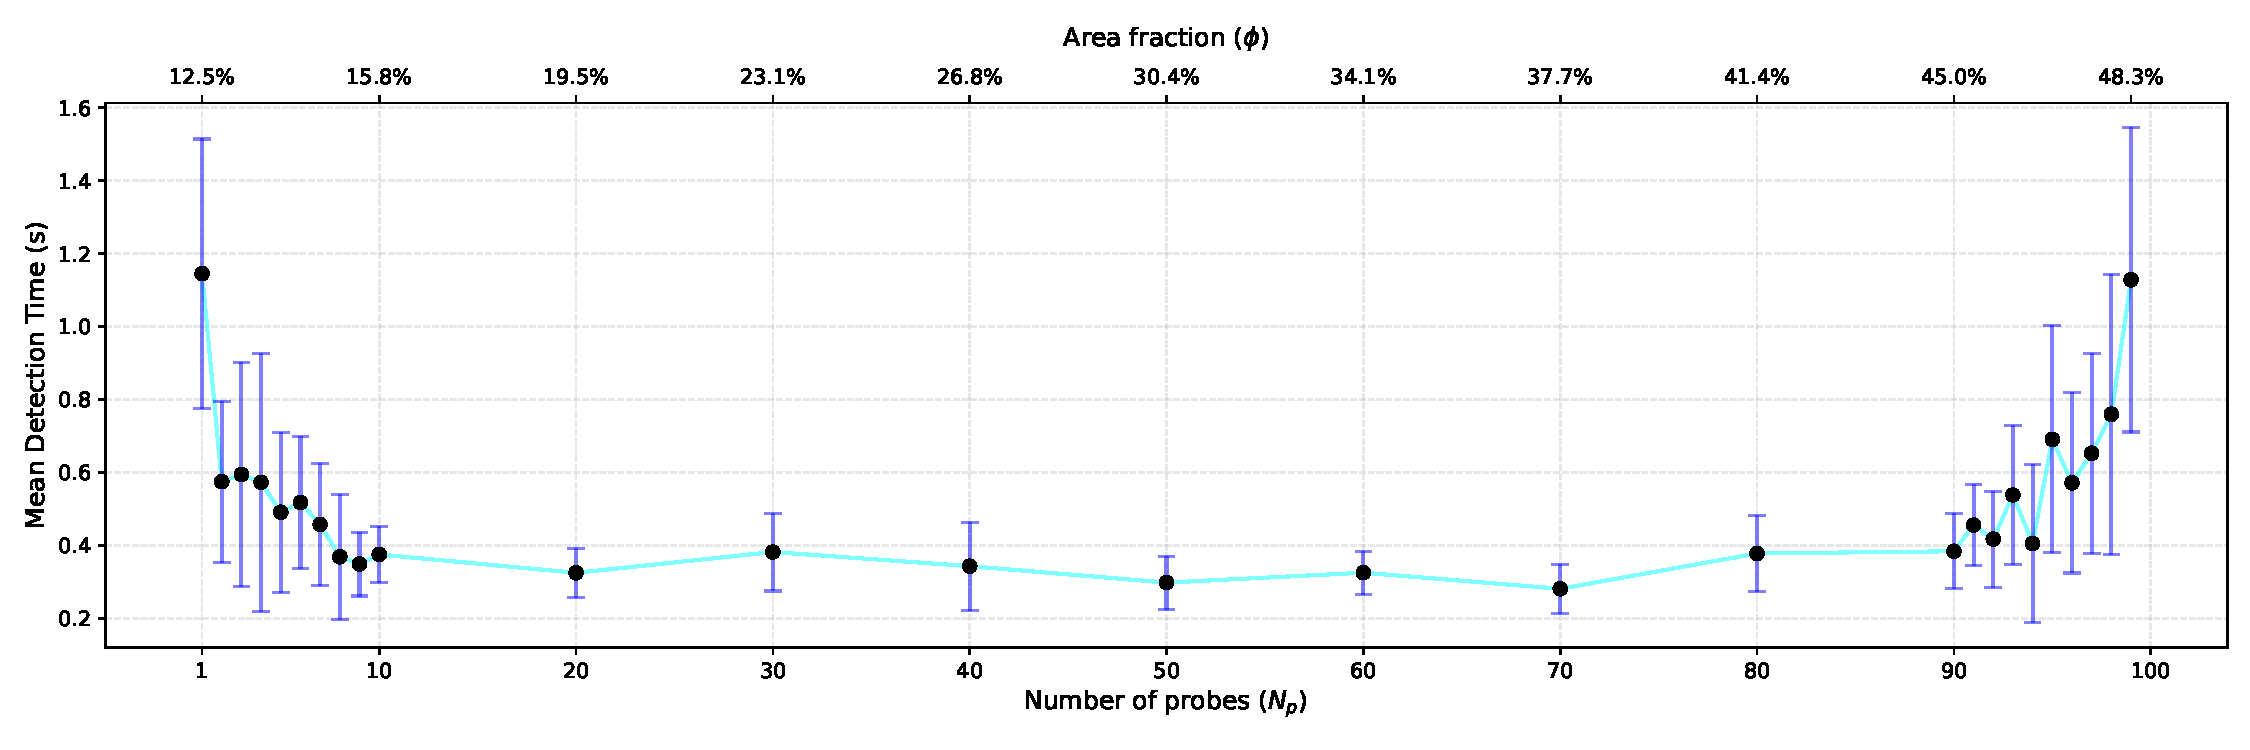
\includegraphics[width=\linewidth]{figures/Detection.pdf}
    \caption{Mean first-passage detection time $\langle T \rangle$ as a function of probe number $N_p$ for a single system of $N_{\text{total}} = 100$ particles. Error bars represent the standard deviation across 10 independent simulation seeds; the top axis shows the corresponding area fraction $\phi$. Reproduced from
    \cite{Balejado2026}.}
    \label{fig:appendix-pa04-fig1}
\end{figure}

Figure~\ref{fig:appendix-pa04-fig1} the same qualitative caldera shape reported in chapter~4 of this thesis: $\langle T \rangle$ falls from $\approx 1.15\,\text{s}$ at $N_p = 1$ at $N_p = 1$ to a minimum of $\approx 0.28\,\text{s}$ near $N_p = 70$ ($\phi \approx 37.7\,\%$), before rising again beyond $N_p \approx 80$-$90$ ($\phi \gtrsim 41$-$45\,\%$) as excluded-volume crowding sets in. This single-system result is consistent with the $N_\text{total} = 100$ system reported in Section~\ref{sec:caldera-fit} (Figure~4.5), whose fitted optimum of $N_p = 48.5$ ($\phi^* \approx 29.9\,\%$) is somewhat lower than the value read directly from the raw minimum in the conference paper, a difference attributable to the caldera model's weighted nonlinear fit smoothing over the noisier, coarser-sampled points near $N_p \approx 90$-$99$ in the original study. The present thesis extends this preliminary observation of a single-system into a systematic sweep over six system sizes and adds the ergodic product $E(N_p)$ and violin-plot distribution diagnostics to the added system sizes to independently confirm and refine the transition.  

\section{Brownian validation LAMMPS code}
{\small
\begin{verbatim}
# Initialization
units si
dimension 2
atom_style sphere

# Box
boundary p p p
region box block 0 5e-6 0 5e-6 -0.001 0.001 units box
create_box 1 box

# Single Particle
create_atoms 1 single 2.5e-6 2.5e-6 0

# Particle Mass
variable density equal 1050
variable radius equal 1e-6  # change to 0.5e-6 for foreign particle
variable volume equal (4/3.0)*3.14159*${radius}^3
variable mass equal ${density}*${volume}
set atom 1 mass ${mass}

# Particle Diameter
set atom 1 diameter 2e-6  # 2 micron diameter

# Dummy Pair Style
pair_style none

fix 1 all langevin 298 298 2.62e-7 78916 # change 2.62e-7 to 1e-7 for foreign

fix 2 all nve/sphere
fix enforce2d all enforce2d

# for computing displacement
compute myDisplacement all displace/atom

# Dump
dump 100 all custom 100 dump.100 id type x y 
\ z vx vy c_myDisplacement[1] c_myDisplacement[2]

thermo 100
timestep 5.00E-08
run 1000000
\end{verbatim}
}

\section{Impurity detection LAMMPS simulation code}
{\small
\begin{verbatim}
# Loop settings

variable Ntotal equal 100 # system_sizes : {10, 30, 50, 70, 100, 200}
variable Lf equal 2.54e-5
#  box sizes: {08.03um, 13.91um, 17.96um , 21.25um, 25.40um, 35.92um}
# seed - depends on how many trials to do
variable seed index 11111, 22222, 33333, 44444, 55555

label loop_seed
  # percentage of probe in the system size
  variable probe_percent index 0.1, 0.2, 0.3, 0.4, 0.5, 0.6, 0.7, 0.8, 0.9, 0.99 
  label loop_percent 
  variable Np_temp equal round(${Ntotal}*${probe_percent})
  if "${Np_temp} < 1" & 
  then "variable Nprobe equal 1" else "variable Nprobe equal ${Np_temp}"
  variable Nmeth equal ${Ntotal}-${Nprobe}

label loop_time
variable run_prod index 10000000 # simulation runtime: 100 mil timesteps = 1 seconds

# Intialization of the system
clear
units si
dimension 2
atom_style sphere
boundary p p p
thermo 1000

# Defining  the Box
variable expand equal 4.0
variable Li equal ${expand}*${Lf}
region box block 0 ${Li} 0 ${Li} -1e-6 1e-6 units box
create_box 2 box

# Particle parameters
variable rho equal 1050.0
variable r equal 1.0e-6
variable d_probe equal 2.0e-6
variable d_meth equal 1.0e-6
variable m equal ${rho}*(4.0/3.0)*PI*${r}^3

# Creating the particles
variable seed_meth equal ${seed}+9876
create_atoms 1 random ${Nprobe} ${seed} box
create_atoms 2 random ${Nmeth}  ${seed_meth} box

set type 1 mass ${m}
set type 2 mass ${m}
set type 1 diameter ${d_probe}
set type 2 diameter ${d_meth}

group probe type 1
group meth  type 2

velocity all set 0.0 0.0 0.0

neighbor 3.0e-6 bin
neigh_modify delay 0 every 1 check yes

# 3 Stage simulation to ensure reliable diffusion
# Optional: First dump - overall dump
# dump dbg all custom 5000 dump_debug_Np${Nprobe}_seed${seed} id type x y vx vy
# dump_modify dbg sort id

# STAGE 1: OVERLAP REMOVAL (SOFT, OVERDAMPED)
timestep 5.0e-8
pair_style soft 3.0e-6
pair_coeff * * 50.0
fix relax all langevin 298 298 1.0e-6 ${seed}
fix lim all nve/limit 1.0e-8
fix e2d all enforce2d
run 50000
unfix relax
unfix lim
unfix e2d

# STAGE 2: COMPRESSION (STILL SOFT)
fix comp all deform 1 x final 0 ${Lf} y final 0 ${Lf} units box remap x
fix relax2 all langevin 298 298 1.0e-6 ${seed}
fix lim2 all nve/limit 1.0e-8
fix e2d2 all enforce2d
run 100000
unfix comp
unfix relax2
unfix lim2
unfix e2d2

# STAGE 3: WCA + BROWNIAN PRODUCTION
timestep 1.0e-8
variable methprobe equal (${d_probe}+${d_meth})/2
variable denominator equal 1.122462

variable sigma11 equal ${d_probe}/${denominator}
variable sigma22 equal ${d_meth}/${denominator}
variable sigma12 equal ${methprobe}/${denominator}
variable rc11 equal 1.122462*${sigma11}
variable rc22 equal 1.122462*${sigma22}
variable rc12 equal 1.122462*${sigma12}

variable ljcut equal ${rc12}
pair_style lj/cut ${ljcut}
pair_modify shift yes
pair_coeff 1 1 1.0e-21 ${sigma11} ${rc11}
pair_coeff 2 2 1.0e-21 ${sigma22} ${rc22}
pair_coeff 1 2 1.0e-21 ${sigma12} ${rc12}

variable seed2 equal ${seed}+12345
fix brown1 probe langevin 298 298 2.62e-7 ${seed} 
fix brown2 meth langevin 298 298 1e-7 ${seed2} 
fix int all nve
fix e2d3 all enforce2d

compute disp all displace/atom
dump prod all custom 100 dump_Ntot${Ntotal}_Np${Nprobe}_Nm${Nmeth}_seed${seed} id type x y
dump_modify prod sort id

run ${run_prod}

#CLEANUP
unfix brown1 
unfix brown2
unfix int
unfix e2d3
undump prod 

# loop Control
  next probe_percent
  jump SELF loop_percent

next seed
jump SELF loop_seed
\end{verbatim}
}















% \hspace{\parindent} You don't need to worry about equations within
% the appendix since \LaTeX automatically formats the equation
% numbers for you. For example,
% \begin{equation}\label{eq:appendixEqn}
%     c^2 = a^2 + b^2
% \end{equation}
% becomes the Pythagorian theorem where $c$ is the length of the
% longest side of any right triangle.

% \section{Codes as appendix}

% \hspace{\parindent}Include your codes when necessary to your
% thesis/dissertation. To do this, you may use \verb+verbatim+
% environment as follows. \textbf{WARNING:} All verbatim and
% verbatiminput environments should always be treated as a separate
% paragraph.  When included in a text paragraph, it sometimes happen
% to reduce the 1.5 spacing to the usual single-spaced text.

% {\small
% \begin{verbatim}
%  #include <iostream>
%  using std::cout;
%  using std::endl;

%  int main( void )
%  {
%     cout << "Hello world!" << endl;
%     return 0;
%  }
% \end{verbatim}
% }

% The \verb+{\small }+ bracketed region is used to lower the font
% size of the entire verbatim text.  This will save you much space
% and give a more aesthetical look in your manuscript.

% On the other hand, when very long codes are wished to be included
% automatically without the tedious cut and paste procedure, you may
% include them using the \verb+\verbatiminput+ command as follows.
% You may want to include a short description of the code of course.

% {\small
%  \verbatiminput{"codes/newC.cpp"}
% }

% This time, you may just include your recent codes by just
% copy-paste-ing the codes (as long they are clean!) into the
% directory \verb$codes/$ in the directory where this file is saved.


\bibliographystyle{plain}
\bibliography{biblio} %% see file: "biblio.bib"
\addcontentsline{toc}{chapter}{Bibliography}

\end{document}
%%end of main.tex
